\documentclass[a4paper, 9pt]{scrartcl}\usepackage[]{graphicx}\usepackage[]{xcolor}
% maxwidth is the original width if it is less than linewidth
% otherwise use linewidth (to make sure the graphics do not exceed the margin)
\makeatletter
\def\maxwidth{ %
  \ifdim\Gin@nat@width>\linewidth
    \linewidth
  \else
    \Gin@nat@width
  \fi
}
\makeatother

\definecolor{fgcolor}{rgb}{0.345, 0.345, 0.345}
\newcommand{\hlnum}[1]{\textcolor[rgb]{0.686,0.059,0.569}{#1}}%
\newcommand{\hlstr}[1]{\textcolor[rgb]{0.192,0.494,0.8}{#1}}%
\newcommand{\hlcom}[1]{\textcolor[rgb]{0.678,0.584,0.686}{\textit{#1}}}%
\newcommand{\hlopt}[1]{\textcolor[rgb]{0,0,0}{#1}}%
\newcommand{\hlstd}[1]{\textcolor[rgb]{0.345,0.345,0.345}{#1}}%
\newcommand{\hlkwa}[1]{\textcolor[rgb]{0.161,0.373,0.58}{\textbf{#1}}}%
\newcommand{\hlkwb}[1]{\textcolor[rgb]{0.69,0.353,0.396}{#1}}%
\newcommand{\hlkwc}[1]{\textcolor[rgb]{0.333,0.667,0.333}{#1}}%
\newcommand{\hlkwd}[1]{\textcolor[rgb]{0.737,0.353,0.396}{\textbf{#1}}}%
\let\hlipl\hlkwb

\usepackage{framed}
\makeatletter
\newenvironment{kframe}{%
 \def\at@end@of@kframe{}%
 \ifinner\ifhmode%
  \def\at@end@of@kframe{\end{minipage}}%
  \begin{minipage}{\columnwidth}%
 \fi\fi%
 \def\FrameCommand##1{\hskip\@totalleftmargin \hskip-\fboxsep
 \colorbox{shadecolor}{##1}\hskip-\fboxsep
     % There is no \\@totalrightmargin, so:
     \hskip-\linewidth \hskip-\@totalleftmargin \hskip\columnwidth}%
 \MakeFramed {\advance\hsize-\width
   \@totalleftmargin\z@ \linewidth\hsize
   \@setminipage}}%
 {\par\unskip\endMakeFramed%
 \at@end@of@kframe}
\makeatother

\definecolor{shadecolor}{rgb}{.97, .97, .97}
\definecolor{messagecolor}{rgb}{0, 0, 0}
\definecolor{warningcolor}{rgb}{1, 0, 1}
\definecolor{errorcolor}{rgb}{1, 0, 0}
\newenvironment{knitrout}{}{} % an empty environment to be redefined in TeX

\usepackage{alltt}
\usepackage[ngerman]{babel}

% -----------------------------------------------------------------------

% -----------------------------------------------------------------------
%% ------------------------------------------------------------
%% by J.Kruppa on Friday, February 11, 2022 (11:31)
%% \def\mainDir{\Sexpr{exam_path}}
\def\source{/Users/jokruppa/source/tex}
\usepackage[margin=2cm, includefoot]{geometry}
\setlength{\parindent}{0cm}
\usepackage{booktabs}
\usepackage{amsmath}
\usepackage{scalerel,amssymb}
\usepackage{setspace}
\def\csquare{{\Large $\boxtimes$}}
\def\msquare{{\Large $\square$}}
\usepackage[normalem]{ulem}
\usepackage{array}
\usepackage{xcolor}
\usepackage{float}
\usepackage{currfile}
\usepackage{tikz}
\usepackage[nomessages]{fp}

%% beamer defs
\def\lecture{Klausurfragen der Bio Data Science}

%% exam defs
\def\examtitle{\lecture}
\def\exammodule{
\vspace{-1.75cm}  
\begin{graybox}{}
\vspace{2Ex}
\textbf{\large Name:} \rule[0ex]{16.75em}{.4pt}
\hfill \textnormal{\textit{Nicht bestanden:}} \msquare \\[2.5Ex]
\textbf{\large Vorname:} \rule[0ex]{15em}{.4pt} \\[2.5Ex]
\textbf{\large Matrikelnummer:} \rule[0ex]{10.8em}{.4pt}
\hfill Endnote: \rule[0ex]{7em}{.4pt} 
\end{graybox}
\vspace{3Ex}
\phantom{text}
}
\def\examsemester{Sommersemester \& Wintersemester}
\def\examdate{\today}
%% ------------------------------------------------------------
\definecolor{darkblue}{rgb}{0,0,.5}
\definecolor{darkpurple}{rgb}{0.4117, 0.2, 0.4117}
\definecolor{uni}{rgb}{0,0.3137,0.6078}
\definecolor{gray}{gray}{0.7}

\usepackage{tcolorbox}
\definecolor{logo1}{RGB}{0, 158, 227}
\definecolor{gray5}{RGB}{247, 247, 247}
\definecolor{gray2}{RGB}{102, 102, 102}

\newtcolorbox{graybox}[1]{
  colback=gray5,%%red!5!white,
  colframe=gray2,%%red!75!black,
  fonttitle=\bfseries\Large,
  %%valign=center,
  fontupper=\large,
  before skip=10pt plus 2pt,
  after skip=20pt plus 4pt,
  title=#1}

\newtcolorbox{takehomebox}[1]{
  colback=gray5,%%red!5!white,
  colframe=logo1,%%red!75!black,
  fonttitle=\bfseries\Large,
  %%valign=center,
  fontupper=\large,
  before skip=10pt plus 2pt,
  after skip=10pt plus 2pt,
  title=#1}

\def\Rlogo{
\includegraphics[width = 0.5cm]{\string~/Documents/GitHub/exam/img/Rlogo}\;}

\usepackage[scaled=.90]{helvet} 
\usepackage{fancyhdr}
\usepackage{lastpage}
\usepackage{hyperref}
\hypersetup{
    colorlinks=true,       % false: boxed links; true: colored links
    linkcolor=black,          % color of internal links 
    urlcolor=magenta           % color of external links
}
\renewcommand{\familydefault}{\sfdefault}

\title{
\large \exammodule \\[5Ex]
\Huge \examtitle \\[2Ex] 
\Large Hochschule Osnabr{\"u}ck
}
\author{Pr{\"u}fer: Prof. Dr. Jochen Kruppa \\
Fakult{\"a}t f{\"u}r Agrarwissenschaften und Landschaftsarchitektur \\ 
j.kruppa@hs-osnabrueck.de}
\date{Version vom \examdate}

%% ------------------------------------------------------------
%% by J.Kruppa on Tuesday, September 23, 2014 (12:50)
%% Header
\renewcommand{\headrulewidth}{0pt}
\renewcommand{\footrulewidth}{0pt}
\pagestyle{fancy}

\fancyhf{}
\fancyhead[L]{}
\fancyhead[R]{}
\fancyfoot[R]{\thepage}
\fancyfoot[L]{\footnotesize \examtitle}

\fancypagestyle{empty}{
 \fancyhf{}
 \fancyhead[L]{}
 \fancyhead[R]{}
 \fancyfoot[R]{\thepage}
 \fancyfoot[L]{\footnotesize \examtitle}
}

\usepackage{arevtext,arevmath}

\newcommand\Tstrut{\rule{0pt}{2.6ex}}         % = `top' strut
\newcommand\Bstrut{\rule[-0.9ex]{0pt}{0pt}}   % = `bottom' strut
\def\strut{\Tstrut\Bstrut}

% -----------------------------------------------------------------------
\IfFileExists{upquote.sty}{\usepackage{upquote}}{}
\begin{document}
\date{Wintersemester 2024/25 
\vfill
\begin{center}

\includegraphics[width = 1.9cm]{avatare/Alex}\hspace{-8mm}

\includegraphics[width = 1.9cm]{avatare/Jessica}\hspace{-8mm}

\includegraphics[width = 1.9cm]{avatare/Jonas}\hspace{-8mm}

\includegraphics[width = 1.9cm]{avatare/Mark}\hspace{-8mm}

\includegraphics[width = 1.9cm]{avatare/Nilufar}\hspace{-8mm}

\includegraphics[width = 1.9cm]{avatare/Paula}\hspace{-8mm}

\includegraphics[width = 1.9cm]{avatare/Steffen}\hspace{-8mm}

\includegraphics[width = 1.9cm]{avatare/Tina}\hspace{-8mm}

\includegraphics[width = 1.9cm]{avatare/Yuki}\\
\small
\vspace{1.5Ex}
\textit{"`The test of a student is not how much he knows,\\ but how much he wants to know."'\\ --- Alice W. Rollins}
\end{center}}
% -----------------------------------------------------------------------
\maketitle
\fancypagestyle{empty}{
  \fancyfoot[L]{\tiny $\square\!\square\!\square\!\square\!\square\!\blacksquare\!\blacksquare\!\square\!\blacksquare\!\square\!\square\!\blacksquare\!\square\!\square\!\blacksquare\!\square\!\blacksquare\!\blacksquare\!\square\!\square$}
}
\thispagestyle{empty}
\clearpage
% -----------------------------------------------------------------------
\begin{minipage}[c]{0.125\textwidth}

\includegraphics[width = 1.9cm]{avatare/Alex}
\end{minipage}
\begin{minipage}[c]{0.875\textwidth}
\textit{Alex studiert im 3. Semester und wiederholt das Modul, da er im ersten Jahr andere Prioritäten für sich gesetzt hat. Das musste sein, da er sich ziemlich im Abitur verausgabt hat. Darüber hinaus war die WG auch eher auf Party angelegt. Alex hofft jetzt über Pünktlichkeit wieder in die Bahn zu kommen. Dafür steht er jetzt immer um 5 Uhr auf! Freunde von ihm beschreiben ihn eher als extrovertiert. Er kennt Paula noch aus der Schulzeit und er überlegt, ob nicht beide Mal nach Mallorca sollten.} 
\end{minipage}\\[2.75Ex]
% -----------------------------------------------------------------------
\begin{minipage}[c]{0.875\textwidth}
\textit{Nach zwei Semestern Studium an der Universität Osnabrück war es dann Jessica doch viel zu theoretisch. Etwas angewandtes sollte es sein, wo sie auch eine Fähigkeit lernt, die frau nutzen kann. Deshalb hat sich Jessica an der Hochschule eingeschrieben. Hoffentlich lernt sie etwas nützliches, wo andere für Geld geben würden. Wer nützlich ist, ist wertvoll. Ihr Traum ist ja eine Hundeschule aufzumachen. Die großen Parties hat sie immer gemieden. Sie ist lieber mit ihrer Hündin im Teuteburgerwald.}
\end{minipage}
\begin{minipage}[c]{0.125\textwidth}

\includegraphics[width = 1.9cm]{avatare/Jessica}
\end{minipage}\\[2.75Ex]
% -----------------------------------------------------------------------
\begin{minipage}[c]{0.125\textwidth}

\includegraphics[width = 1.9cm]{avatare/Jonas}
\end{minipage}
\begin{minipage}[c]{0.875\textwidth}
\textit{Das ist jetzt der letzte Versuch mit einem Studium. Wenn es nicht klappt dann überlegt Jonas das \href{https://www.ihk.de/osnabrueck/aus-und-weiterbildung/ausbildung/ausbildungsbetriebe/projekt-neustart-1087206}{Programm der IHK zu Ausbildungsvermittlung} zu nutzen. Aber eine Runde gibt er sich noch. Struktur ist eigentlich das Wichtigste und diesmal hat er sich alle Altklausuren der Fachschaft besorgt. Dann ist er auch noch gleich der Fachschaft beigetreten um mehr Informationen abzugreifen. Und er versucht nicht seine Zeit mit Alex zu verdaddeln oder in der Fachschaft bei einem Bier oder so...}
\end{minipage}\\[2.75Ex]
% -----------------------------------------------------------------------
\begin{minipage}[c]{0.875\textwidth}
\textit{Nächstes Semester geht es nach Kanada davon hat er schon auf der Berufsschule geträumt. Deshalb konzentriert er sich sehr auf die Prüfungen. Ein Schiff ist im Hafen sicher, aber dafür ist es nicht gebaut worden. Das \href{https://www.hs-osnabrueck.de/wir/fakultaeten/aul/international/}{International Faculty Office} der Fakultät Agrarwissenschaften und Landschaftsarchitektur hat super geholfen, aber es waren einiges an Unterlagen. Jetzt hofft er, dass Tina dann doch noch mitkommt. Aber sonst macht er das eben alleine. Obwohl das eher nicht so seine Art ist. Vielleicht sollte er sich mal einen Tipp bei Tina holen, sie wirkt sehr entschlossen.} 
\end{minipage}
\begin{minipage}[c]{0.125\textwidth}

\includegraphics[width = 1.9cm]{avatare/Mark}
\end{minipage}\\[2.75Ex]
% -----------------------------------------------------------------------
\begin{minipage}[c]{0.125\textwidth}

\includegraphics[width = 1.9cm]{avatare/Nilufar}
\end{minipage}
\begin{minipage}[c]{0.875\textwidth}
\textit{Nach der Ausbildung wollte Nilufar eigentlich gleich anfangen zu arbeiten, aber nach einem Praktikum und der Probezeit stellte sie fest, dass es ohne einen Hochschulabschluss schwer wird Führungsverantwortung zu übernehmen. Mit Menschen kann sie schon immer und dann auch eigene Projekte mit anderen verwirklichen, dass ist doch was. Mit dem notwendigen Abschluss sollte der Start um so einfacher sein. Dann ist sie keine Befehlsempfängerin mehr sondern gibt die Marschrichtung vor. Schon jetzt koordiniert Nilufar das Studium von anderen.}
\end{minipage}\\[2.75Ex]
% -----------------------------------------------------------------------
\begin{minipage}[c]{0.875\textwidth}
\textit{Paula möchte die Welt zu einem besseren Ort machen. Wenn da nicht die anderen Mitmenschen wären. Paula muss das Modul nochmal wiederholen, da es dann am Ende des Semesters zu viel für sie wurde. Eine Lerngruppe hätte geholfen, aber das ist dann gar nicht so einfach eine zu finden. Zwar kennt sie schon Nilufar, aber Nilufar ist ihr manchmal zu forsch. Ihr schwant aber, dass alleine das Studium sehr schwer werden wird. Das Abitur war schon so ein Lernhorror, das möchte sie nicht nochmal. Alex sieht sie da als Vorbild.}
\end{minipage}
\begin{minipage}[c]{0.125\textwidth}

\includegraphics[width = 1.9cm]{avatare/Paula}
\end{minipage}\\[2.75Ex]
% -----------------------------------------------------------------------
\begin{minipage}[c]{0.125\textwidth}

\includegraphics[width = 1.9cm]{avatare/Steffen}
\end{minipage}
\begin{minipage}[c]{0.875\textwidth}
\textit{Sommer, Sonne, Natur. Das ist es was Steffen mag. Raus in die Komune und die Natur genießen. Leider hat Steffen noch andere Bedürfnisse, die ein Einkommen benötigen. Da Studierte mehr verdienen, würde dann in Teilzeit auch mehr rausspringen. Wenn er dann privat was anbauen kann, dann spart er gleich doppelt. Leider sind viele seiner Kommilitonen total verkrampfte Karrieristen. Es geht nur ums Äußere. Dabei verliert sich Steffen gerne im Prozess. Das hat auch seinen Schulabschluss etwas verzögert. Steffen lässt sich eben Zeit.}
\end{minipage}\\[2.75Ex]
% -----------------------------------------------------------------------
\begin{minipage}[c]{0.875\textwidth}
\textit{Wille  war es, die es Tina hierher gebracht hat und Wille wird es sein, die Tina dann auch zum Abschluß treibt. Nach einem Rückschlag muss Tina jetzt einige Module wiederholen, damit sie dann auch fertig wird. Ab und zu ist sie schwach gewesen und das hat dann Zeit gekostet. Das Tina es dann manchmal übertreibt, weiß sie nur zu gut, aber irgendwie muss die Kontrolle ja erhalten bleiben? Insbesondere, wenn sie mal wieder die Nacht durchgefeiert hat, verachtet Tina sich. Dann baut Nilufar sie dann bei einem Tee wieder auf.}
\end{minipage}
\begin{minipage}[c]{0.125\textwidth}

\includegraphics[width = 1.9cm]{avatare/Tina}
\end{minipage}\\[2.75Ex]
% -----------------------------------------------------------------------
\begin{minipage}[c]{0.125\textwidth}

\includegraphics[width = 1.9cm]{avatare/Yuki}
\end{minipage}
\begin{minipage}[c]{0.875\textwidth}
\textit{Für Yuki war es nicht einfach. Teilweise war die Krankheit sehr hinderlich, dann war es Yuki selber. Dann muss man auch wieder auf die Beine kommen und es dauert eben seine Zeit. Aber immerhin hat Yuki es jetzt den Abschluss gekriegt und hat einen Studienplatz. Jetzt heißt es in den Rhythmus kommen und schauen, was noch so passiert. Immerhin hat Yuki schon eine kleine Gruppe gefunden, in der Yuki dann Hilfe findet. Ist aber auch sehr unübersichtlich so ein Studium. Steffen ist immer super entspannt.}
\end{minipage}
\clearpage
% -----------------------------------------------------------------------


\begin{graybox}{Erlaubte Hilfsmittel}
  \vspace{1Ex}
  \begin{itemize}
  \item Normaler Taschenrechner ohne Möglichkeit der Kommunikation mit anderen
    Geräten! Ausdrücklich kein Handy!
  \item Eine DIN A4-Seite als beidseitig, selbstgeschriebene,
    handschriftliche Formelsammlung. Keine digitalen Ausdrucke! 
  \item \textbf{\textcolor{red}{Die Verwendung eines roten Farbstiftes ist nicht gestattet! Korrekturfarbe!}}
  \item \textit{You can answer the questions in English without any consequences.}  
  \end{itemize}
\end{graybox}
\vfill

\begin{graybox}{Endnote}
  \vspace{1Ex}
  \begin{itemize}
  \item[] \rule[0ex]{3em}{.4pt}\, von 20\, Punkten sind aus den Multiple
    Choice Aufgaben erreicht.
  \item[] \rule[0ex]{3em}{.4pt}\, von 75 Punkten sind aus den Rechen- und
    Textaufgaben erreicht. 
  \item[] \rule[0ex]{3em}{.4pt}\, von 95 Punkten in Summe.
  \item[] Es wird folgender Notenschlüssel angewendet.   
  \end{itemize}
  \vspace{1ex}
\begin{center}
  \begin{tabular}[c]{cc}
    \toprule
    \textbf{Punkte}	&	\textbf{Note}	\\
    \midrule
    91.0 - 95.0	&	1,0	\\
    86.0 - 90.5	&	1,3	\\
    81.5 - 85.5	&	1,7	\\
    76.5 - 81.0	&	2,0	\\
    72.0 - 76.0	&	2,3	\\
    67.5 - 71.5	&	2,7	\\
    62.5 - 67.0	&	3,0	\\
    58.0 - 62.0	&	3,3	\\
    53.0 - 57.5	&	3,7	\\
    47.5 - 52.5	&	4,0	\\
    \bottomrule
  \end{tabular}
\end{center}
  \vspace{1ex}
\begin{itemize}
\item[] Es ergibt sich eine Endnote von \rule[0ex]{4em}{.4pt}.
\end{itemize}
  \vspace{1Ex}
\end{graybox}

% -----------------------------------------------------------------------
\newpage
% -----------------------------------------------------------------------

\begin{graybox}{Multiple Choice Aufgaben}
  \begin{itemize}
  \item Pro Multipe Choice Frage ist \emph{genau} eine Antwort richtig.
  \item \textbf{Übertragen Sie Ihre Kreuze in die Tabelle auf
      dieser Seite.}
  \end{itemize}

\begin{center}
  \large
  \begin{tabular}{|l|c|c|c|c|c?c|}
    \hline
    & \textbf{A} & \textbf{B} & \textbf{C} & \textbf{D} & \textbf{E} & $\boldsymbol{\checkmark}$\strut\\
    \hline
    \textbf{Aufgabe 1} &   &   &   &   &   & \strut\\
    \hline
    \textbf{Aufgabe 2} &   &   &   &   &   & \strut\\
    \hline
    \textbf{Aufgabe 3} &   &   &   &   &   & \strut\\
    \hline
    \textbf{Aufgabe 4} &   &   &   &   &   & \strut\\
    \hline
    \textbf{Aufgabe 5} &   &   &   &   &   & \strut\\
    \hline
    \textbf{Aufgabe 6} &   &   &   &   &   & \strut\\
    \hline
    \textbf{Aufgabe 7} &   &   &   &   &   & \strut\\
    \hline
    \textbf{Aufgabe 8} &   &   &   &   &   & \strut\\
    \hline
    \textbf{Aufgabe 9} &   &   &   &   &   & \strut\\
    \hline
    \textbf{Aufgabe 10} &   &   &   &   &   & \strut\\
    \hline
  \end{tabular}
\end{center}

\begin{itemize}
\item Es sind \rule[0ex]{2em}{.4pt}\, von 20 Punkten erreicht worden.
\end{itemize}
\end{graybox}

\vfill

\begin{graybox}{Rechen- und Textaufgaben}
  \begin{center}
    \large
    \begin{tabular}{|l|c|c|c|c|c|c|c|}
      \hline
      \textbf{Aufgabe} & \textbf{11} & \textbf{12} & \textbf{13} & \textbf{14} & \textbf{15} & \textbf{16} & \textbf{17} \strut\\
      \hline
      \textbf{Punkte} & 
      \hspace{1Ex}\Large\textcolor{gray!70}{10}\hspace{1Ex}  & 
      \hspace{1Ex}\Large\textcolor{gray!70}{12}\hspace{1Ex}  & 
      \hspace{1Ex}\Large\textcolor{gray!70}{9}\hspace{1Ex}  & 
      \hspace{1Ex}\Large\textcolor{gray!70}{12}\hspace{1Ex}  & 
      \hspace{1Ex}\Large\textcolor{gray!70}{12}\hspace{1Ex}  & 
      \hspace{1Ex}\Large\textcolor{gray!70}{10}\hspace{1Ex}  & 
      \hspace{1Ex}\Large\textcolor{gray!70}{10}\hspace{1Ex} \strut\\
      \hline
  \end{tabular}
\end{center}
\begin{itemize}
\item Es sind \rule[0ex]{2em}{.4pt}\, von 75 Punkten erreicht worden.
\end{itemize}
\end{graybox}

% -----------------------------------------------------------------------
\clearpage
% -----------------------------------------------------------------------
\begin{graybox}{Multiple Choice Aufgaben}
Die Multiple Choice Aufgaben \textcolor{red}{unterliegen dem Zufall}. Die Reihenfolge der Antworten ist zufällig. Die Fragen und Antworten sind semantisch zufällig und haben somit \textcolor{red}{verschiedene Textvarianten}. Insbesondere die reinen Textaufgaben haben verschiedene Textvarianten. Die Semeantik mag sich unterscheiden, die Inhalte sind aber gleich.
\end{graybox}
\section*{ANOVA}

\section{Aufgabe \hfill (2 Punkte)}





Sie führen einen Versuch mit einer Behandlung und drei Faktorleveln durch. Danach rechnen Sie eine einfaktorielle ANOVA und es ergibt sich ein $\eta^2 = 0.52$. Welche Aussage ist richtig?



\begin{enumerate}
\item [\textbf{A} \msquare] Das $\eta^2$ ist die Korrelation der ANOVA. Mit der Ausnahme, dass 0 der beste Wert ist.
\item [\textbf{B} \msquare] Das $\eta^2$ ist ein Wert f{"u}r die G{"u}te der ANOVA. Je kleiner desto besser. Ein $\eta^2$ von 0 bedeutet ein perfektes Modell mit keiner Abweichung. Die Varianz ist null.
\item [\textbf{C} \msquare] Die Berechnung von $\eta^2$ ist ein Wert f{"u}r die Interaktion.
\item [\textbf{D} \msquare] Das $\eta^2$ beschreibt den Anteil der Varianz, der von den Behandlungsbedingungen nicht erkl{"a}rt wird. Somit der Rest an nicht erkl{"a}rbarer Varianz.
\item [\textbf{E} \msquare] Das $\eta^2$ ist damit mit dem $R^2$ aus der linearen Regression zu vergleichen und beschreibt den Anteil der Varianz, der von den Behandlungsbedingungen erkl{"a}rt wird.
\end{enumerate} 

\section{Aufgabe \hfill (2 Punkte)}



Sie führen ein Feldexperiment durch um das Gewicht von Brokoli zu
steigern. Die Pflanzen wachsen unter einer Kontrolle und zwei verschiedenen
Behandlungsbedingungen. Nach der Berechnung einer einfaktoriellen ANOVA
ergibt sich ein $\eta^2 = 0.24$. Welche Aussage ist richtig?



\begin{enumerate}
\item [\textbf{A} \msquare] Mit dem $\eta^2$ lässt sich auf die Qualität der Randomisierung und damit der Strukturgleichheit zwischen der Grundgesamtheit und der Stichprobe schließen. Es gilt dabei die Regel, dass ein $\eta^2$-Wert von 1 zu bevorzugen ist.
\item [\textbf{B} \msquare] Es werden 24\% der Varianz durch den Versuch erklärt. Das $\eta^2$ beschreibt den Anteil der Varianz, der durch Fehler in der Versuchsdurchführung entsteht.
\item [\textbf{C} \msquare] Das $\eta^2$ beschreibt den Anteil der Varianz, der durch den Forschenden entsteht. Es gilt die Regel, dass ca. 70\% der Varianz eines Versuches durch die Versuchsdurchführung entstehen sollen.
\item [\textbf{D} \msquare] Es werden 24\% der Varianz durch die Behandlung erklärt. Das $\eta^2$ beschreibt den Anteil der Varianz, der von den unterschiedlichen Behandlungsbedingungen erklärt wird.
\item [\textbf{E} \msquare] Es werden 76\% der Varianz durch die Behandlung erklärt. Das $\eta^2$ beschreibt den Anteil der Varianz, der von den unterschiedlichen Behandlungsbedingungen nicht erklärt wird.
\end{enumerate} 

\section{Aufgabe \hfill (2 Punkte)}



Eine einfaktorielle ANOVA berechnet eine Teststatistik um zu die Nullhypothese abzulehnen. Welche Aussage über die Teststatistik der ANOVA ist richtig?



\begin{enumerate}
\item [\textbf{A} \msquare] Die ANOVA berechnet die T-Statistik indem den Mittelwertsunterschied der Gruppen simultan durch die Standardabweichung der Gruppen teilt. Wenn die T-Statistik h{"o}her als 1.96 ist, kann die Nullhypothese abgelehnt werden.
\item [\textbf{B} \msquare] Wenn die F-Statistik höher ist als der kritische Wert kann die Nullhypothese nicht abgelehnt werden. Die F-Statistik ist die Differenz der MS der Behandlung durch die MS des Fehlers.
\item [\textbf{C} \msquare] Die ANOVA berechnet die T-Statistik aus der Multiplikation der MS Behandlung mit der MS der Fehler. Wenn die F-Statistik genau 0 ist, kann die Nullhypothese nicht abgelehnt werden.
\item [\textbf{D} \msquare] Die ANOVA berechnet die F-Statistik indem die MS des Fehlers durch die MS der Behandlung geteilt werden. Wenn die F-Statistik sich der 0 ann{"a}hert kann die Nullhypothese abgelehnt werden.
\item [\textbf{E} \msquare] Die ANOVA berechnet die F-Statistik indem die MS der Behandlung durch die MS des Fehlers geteilt werden. Wenn die F-Statistik sich der 0 ann{"a}hert kann die Nullhypothese nicht abgelehnt werden.
\end{enumerate} 

\section{Aufgabe \hfill (2 Punkte)}




Viele statistische Verfahren nutzen eine Teststatistik um eine Aussage über den Zusammenhang zwischen der Grundgesamthat und der Stichprobe abzubilden. Ein statistisches Testwerkzeug ist hierbei die ANOVA. Die ANOVA rechnet dabei...



\begin{enumerate}
\item [\textbf{A} \msquare] ... den Unterschied zwischen der Varianz durch verschiedene Behandlungsguppen unter der Varianz über alle Behandlungsgruppen. Wenn die ANOVA signifikant ist, kann kein Effekt $\eta^2$ bestimmt werden.
\item [\textbf{B} \msquare] ... den Unterschied zwischen der F-Statistik anhand der Varianz der Gruppen. Wenn die F-Statistik exakt 0 ist, kann die Nullhypothese abgelehnt werden.
\item [\textbf{C} \msquare] ... den Unterschied zwischen der Mittelwerte und der Varianz aus verschiedenen Behandlungsguppen. Wenn die ANOVA signifikant ist, ist bekannt welcher Vergleich konkret unterschiedlich ist.
\item [\textbf{D} \msquare] ... den Unterschied zwischen der Varianz über alle Behandlungsgruppen oder der Varianz aus verschiedenen Behandlungsguppen. Wenn die ANOVA signifikant ist, muss sich zwischen einem der beiden Varianzquellen entschieden werden.
\item [\textbf{E} \msquare] ... den Unterschied zwischen der Varianz aus verschiedenen Behandlungsguppen und der Varianz über alle Behandlungsgruppen. Wenn die ANOVA signifikant ist, muss über einen Posthoc-Test nachgedacht werden um den signifikanten Unterschied in den Gruppen exakt zu bestimmen.
\end{enumerate} 

\section{Aufgabe \hfill (2 Punkte)}



In einer Studie zur Bewertung der Wirkung von Vitamin C auf das Zahnwachstum bei Igeln entstand folgende Abbildung. Der Versuch wurde an 52 Tieren durchgeführt, wobei jedes Tier eine von  drei Vitamin-C-Dosen (0.5, 1 und 1.5 mg/Tag) über eine von zwei Verabreichungsmethoden erhielt. Welche Aussage ist im Bezug auf eine zweifaktorielle ANOVA richtig?



{\centering 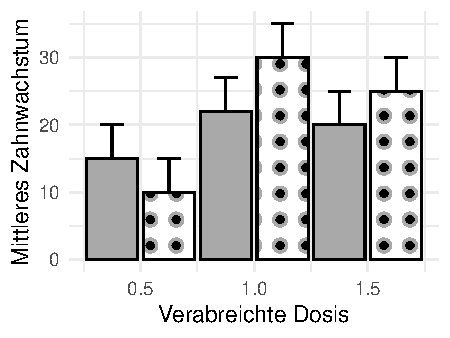
\includegraphics[width=\maxwidth]{img/mc-anova-02-a-1} 

}







\begin{enumerate}
\item [\textbf{A} \msquare] Das Bestimmtheitsmaß $R^2$ ist groß.
\item [\textbf{B} \msquare] Keine Interaktion liegt vor $(p \leq 0.05)$.
\item [\textbf{C} \msquare] Eine mittlere bis starke Interaktion liegt vor $(p \leq 0.05)$
\item [\textbf{D} \msquare] Die Koeffizienten sind positiv $(\beta_0 > 0; \beta_1 > 0)$.
\item [\textbf{E} \msquare] Eine negative Interaktion liegt vor $(\rho \geq 0.5)$.
\end{enumerate} 
\section*{Deskriptive Statistik \& Explorative Datenanalyse}

\section{Aufgabe \hfill (2 Punkte)}




Gegeben ist $y$ mit 13, 11, 6, 9 und 10. Berechnen Sie den Mittelwert und Standardabweichung.



\begin{enumerate}
\item [\textbf{A} \msquare] Es ergibt sich 9.8 +/- 2.59
\item [\textbf{B} \msquare] Es ergibt sich 8.8 +/- 3.35
\item [\textbf{C} \msquare] Es ergibt sich 10.8 +/- 1.295
\item [\textbf{D} \msquare] Es berechnet sich 9.8 +/- 6.7
\item [\textbf{E} \msquare] Sie erhalten 9.8 +/- 1.295
\end{enumerate} 

\section{Aufgabe \hfill (2 Punkte)}




Wie lautet der Median, das $1^{st}$ Quartile sowie das $3^{rd}$ Quartile von $y$ mit 35, 24, 19, 21, 18, 30, 16, 22, 20, 10 und 51.




\begin{enumerate}
\item [\textbf{A} \msquare] Es ergibt sich 24 +/- 18
\item [\textbf{B} \msquare] Es berechnet sich 24 [19; 31]
\item [\textbf{C} \msquare] Es berechnet sich 22 [19; 29]
\item [\textbf{D} \msquare] Sie erhalten 21 [16; 28]
\item [\textbf{E} \msquare] Es berechnet sich 21 [18; 30]
\end{enumerate} 

\section{Aufgabe \hfill (2 Punkte)}



Die empfohlene Mindestanzahl an Beobachtungen für die Visualisierung mit einem Histogramm sind...



\begin{enumerate}
\item [\textbf{A} \msquare] Die untere Grenze liegt bei einer Beobachtung.
\item [\textbf{B} \msquare] Die opimale Anzahl ist größer als hundert Beobachtungen, wobei es gerne sehr viel mehr sein können.
\item [\textbf{C} \msquare] 1 Beobachtung.
\item [\textbf{D} \msquare] Wir sollten eine Beobachtung mindestens pro Gruppe vorliegen haben.
\item [\textbf{E} \msquare] Damit wir hier sauber eine Abbilung von einem 
\end{enumerate}

\section{Aufgabe \hfill (2 Punkte)}



Sie wollen nach einem Feldversuch die Standardabweichung berechnen. Welche der folgenden Rechenoperationen müssen durchgeführt werden?



\begin{enumerate}
\item [\textbf{A} \msquare] Den Mittelwert berechnen und die Abstände quadrieren. Die Summe mit der Fallzahl multiplizieren.
\item [\textbf{B} \msquare] Den Mittelwert berechen, dann die quadratischen Abstände zum Mittelwert aufsummieren und durch die Fallzahl teilen, dann die Wurzel ziehen.
\item [\textbf{C} \msquare] Als erstes berechnen wir den Mittelwert. Dann bilden wir die Summe der quadratischen Abstände zu dem Mittelwert. Abschließend teilen wir durch die Fallzahl.
\item [\textbf{D} \msquare] Als erstes berechnen wir den Mittelwert. Dann bilden wir die Summe der quadratischen Abstände zu dem Mittelwert. Abschließend subtrahieren wir die Fallzahl.
\item [\textbf{E} \msquare] Wir berechnen erst den Mittelwert und dann die absoluten Abstände zu dem Mittelwert. Diese quadratischen Abstände summieren wir auf und teilen am Ende durch die Fallzahl.
\end{enumerate} 

\section{Aufgabe \hfill (2 Punkte)}



In Ihrer Abschlußarbeit wolllen Sie Ihre Daten für den Ertrag in einem Boxplot darstellen. Sie nutzen den Boxplot auch, da der Boxplot zu den meist genutzten Visualiserungen von Daten gehört. Welche statistischen Maßzahlen stellt der Boxplot dar?

 



\begin{enumerate}
\item [\textbf{A} \msquare] Durch die Abbildung des Boxplot erhalten wir die Informationen über die Mittelwerte und die Standardabweichung.
\item [\textbf{B} \msquare] Der Boxplot stellt den Median und die Streuung dar.
\item [\textbf{C} \msquare] Der Boxplot stellt den Median und die Quartile dar.
\item [\textbf{D} \msquare] Den Mittelwert sowie den Median und die Streuung.
\item [\textbf{E} \msquare] Der Boxplot stellt die Mittelwerte und die Varianz dar.
\end{enumerate}

\section{Aufgabe \hfill (2 Punkte)}



Nachdem Sie in einem Feldexperiment zu Leistungssteigerung von Maiss durchgeführt haben, berechnen Sie den Mittelwert und den Median. Der Mittelwert $\bar{y}$ und der Median $\tilde{y}$ unterscheiden sich. Welche Aussage ist richtig?



\begin{enumerate}
\item [\textbf{A} \msquare] Da sich der Mittelwert und der Median nicht unterscheiden, liegen vermutlich keine Outlier in den Daten vor. Wir verweden den Datensatz so wie er ist.
\item [\textbf{B} \msquare] Da sich der Mittelwert und der Median nicht unterscheiden, liegen vermutlich Outlier in den Daten vor. Wir untersuchen den Datensatz nach auffälligen Beobachtungen.
\item [\textbf{C} \msquare] Da sich der Mittelwert und der Median unterscheiden, liegen vermutlich Outlier in den Daten vor. Wir untersuchen den Datensatz nach auffälligen Beobachtungen.
\item [\textbf{D} \msquare] Wenn sich der Mittelwert und der Median nicht unterscheiden, liegen vermutlich Outlier in den Daten vor.
\item [\textbf{E} \msquare] Da sich der Mittelwert und der Median unterscheiden, ist der Datensatz nicht zu verwenden. Mittelwert und Median müssen gleich sein.
\end{enumerate}

\section{Aufgabe \hfill (2 Punkte)}



Sie wollen eine ANOVA im Anschluss an Ihr Feldexperiment rechnen. Dafür muss Ihr gemessener Endpunkt die Annahme einer Varianzhomogenität genügen. Zur Überprüfung können Sie folgende Visualisierung nutzen. Welche entsprechende Regel zur Abschätzung der Annahme einer Varianzhomogenität kommt zur Anwendung?



\begin{enumerate}
\item [\textbf{A} \msquare] Nach dem Einlesen der Daten nutzen wir einen Barplot um zu schauen, ob alle Mittelwerte über alle Behandlungen in etwa gleich groß sind. Damit ist dann auch die Varianz in allen Behandlungen in etwa gleich.
\item [\textbf{B} \msquare] In einer explorativen Datanalyse nutzen wir den Boxplot. Dabei sollte der Median als dicke Linie in der Mitte der Box liegen. Dann können wir von einer Varianzhomogenität ausgehen.
\item [\textbf{C} \msquare] Einen Barplot. Die Mittelwerte müssen alle auf einer Höhe liegen. Die Fehlerbalken haben hier keine Informationen.
\item [\textbf{D} \msquare] Wir erstellen uns für jede Behandlung einen Dotplot und schauen, ob die Dots und damit die Varianz für jede Behandlung gleich groß sind.
\item [\textbf{E} \msquare] Nach dem Einlesen der Daten nutzen wir einen Boxplot um zu schauen, ob alle Boxen über alle Behandlungen in etwa gleich groß sind. Damit ist dann auch das IQR in allen Behandlungen in etwa gleich.
\end{enumerate}

\section{Aufgabe \hfill (2 Punkte)}




In der Statistik müssen wir häufig überprüfen, ob unser Outcome einer bestimmten Verteilung folgt. Meistens überprüfen wir, ob eine
Normalverteilung vorliegt. Folgende drei Abbildungen eigenen sich im Besonderen für die Überprüfung einer Verteilungsannahme an eine Variable.





\begin{enumerate}
\item [\textbf{A} \msquare] Scatterplot, Densityplot, Barplot
\item [\textbf{B} \msquare] Histogramm, Scatterplot, Boxplot
\item [\textbf{C} \msquare] Violinplot, Scatterplot, Barplot
\item [\textbf{D} \msquare] Histogramm, Densityplot, Dotplot
\item [\textbf{E} \msquare] Boxplot, Densityplot, Violinplot
\end{enumerate} 

\section{Aufgabe \hfill (2 Punkte)}



Bevor Sie in Ihrer Abschlussarbeit einen statistischen Test rechnen, wollen Sie einmal betrachten, welcher Verteilung Ihre $n = 200$ geernteten Pflanzen folgen.  Welche Verteilung ist abgebildet?



{\centering 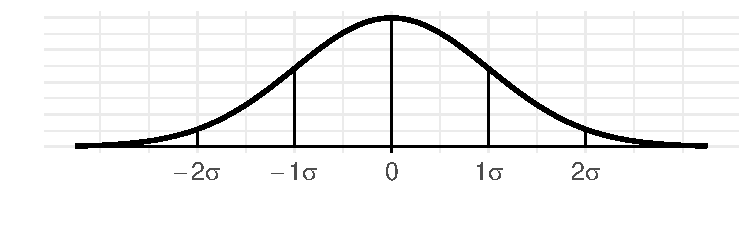
\includegraphics[width=\maxwidth]{img/mc-distribution-02-a-1} 

}







\begin{enumerate}
\item [\textbf{A} \msquare] In dem Histogramm ist eine Normalverteilung dargestellt.
\item [\textbf{B} \msquare] In dem Histogramm ist eine Ordinalverteilung dargestellt.
\item [\textbf{C} \msquare] Wir haben eine Gammaverteilung vorliegen.
\item [\textbf{D} \msquare] Es handelt sich um eine Poisson-Verteilung.
\item [\textbf{E} \msquare] Eine Standardnormalverteilung.
\end{enumerate} 
\section*{Lineare Regression \& Korrelation}

\section{Aufgabe \hfill (2 Punkte)}



In Ihrer Abschlussarbeit wollen Sie ein kausales Modell rechnen. Jetzt stellt sich die Frage, was diese Entscheidung für Ihre Auswertung bedeutet. Welche Aussage ist richtig?



\begin{enumerate}
\item [\textbf{A} \msquare] Wir modellieren den Zusammenhang zwischen $X$ und $Y$ wenn ein kausales Modell rerechnet wird. Dabei kann nicht der gesamte Datensatz genutzt werden. Es wird ein Trainingsdatensatz zum Trainieren des Modells benötigt.
\item [\textbf{B} \msquare] Ein kausales Modell möchte die Zusammenhänge von X auf Y modellieren. Hierbei geht es um die Effekte von $X$ auf $Y$. Man sagt, wenn $x_1$ um 1 ansteigt ändert sich $Y$ um einen Betrag $\beta_1$.
\item [\textbf{C} \msquare] Wenn ein kausales Modell gerechnet werden soll, dann muss zum einen ein Traingsdatensatz sowie ein Testdatensatz definiert werden. Dabei ist der Trainingsdatensatz meist 1/10 und der Testdatensatz 1/3 der Fallzahl groß. Der Testdatensatz dient zur Validierung.
\item [\textbf{D} \msquare] Wenn ein kausales Modell gerechnet werden soll, dann muss zum einen ein Traingsdatensatz sowie ein Testdatensatz definiert werden. Dabei ist der Trainingsdatensatz meist 2/3 und der Testdatensatz 1/3 der Fallzahl groß. Der Testdatensatz dient zur Validierung.
\item [\textbf{E} \msquare] Ein kausales Modell wird auf einem Trainingsdatensatz trainiert und anschliessend über eine explorative Datenanalyse validiert. Signifikanzen über $\beta_i$ können hier nicht festgestellt werden.
\end{enumerate}

\section{Aufgabe \hfill (2 Punkte)}



Nach einer Regressions sollten die Residuen normalverteilt sein. Was bei einer simplen Regression noch relativ einfach visuell in einem Scatterplot zu überprüfen ist. Für komplexere Modell liefert der QQ-Plot die notwendigen Informationen über die Normalverteilung. Welche Aussage ist richtig?



{\centering 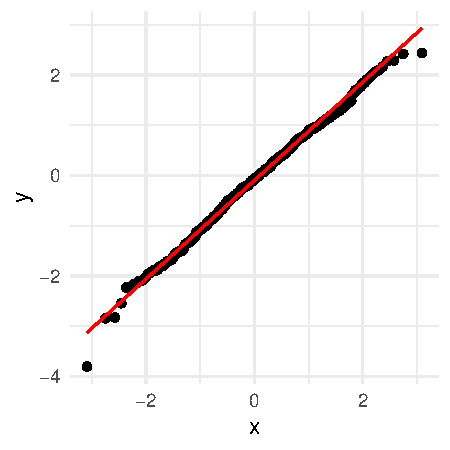
\includegraphics[width=\maxwidth]{img/mc-regression-05-a-1} 

}







\begin{enumerate}
\item [\textbf{A} \msquare] Die Annahme der normalverteilten Residuen ist erfüllt. Die Punkte liegen zum überwiegenden Teil nicht auf der Geraden und Korrelation ist negativ.
\item [\textbf{B} \msquare] Die Annahme der normalverteilten Residuen ist nicht erfüllt. Die Punkte liegen zum überwiegenden Teil nicht auf der Geraden.
\item [\textbf{C} \msquare] Wir betrachten die Gerade und dabei insbesondere die beiden Enden der Gerade. Hier sollten die Punkte auf der Geraden liegen, dann ist die Annahme an die Normalverteilung der Residuen erfüllt.
\item [\textbf{D} \msquare] Die Annahme der normalverteilten Residuen ist erfüllt. Die Punkte liegen zum überwiegenden Teil nicht auf der Geraden.
\item [\textbf{E} \msquare] Wir betrachten die Gerade. Wenn die Punkte einigermaßen gleichmäßig um die Gerade verteilt liegen, dann gehen wir von normalverteilten Residuen aus. Dies ist hier nicht der Fall. Wir haben keine normalverteilten Residuen vorliegen.
\end{enumerate}

\section{Aufgabe \hfill (2 Punkte)}



Nach der Modellierung einer Regression stellt sich die Frage, ob die Residuen (\texttt{.resid}) gleichmäßig um die gefitte Gerade liegen. Sie können folgende Abbildung für die visuelle Überprüfung der Residuen nutzen. Welche Aussage ist richtig?



{\centering 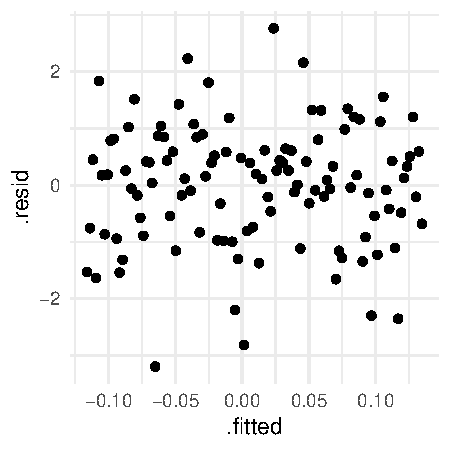
\includegraphics[width=\maxwidth]{img/mc-regression-06-a-1} 

}







\begin{enumerate}
\item [\textbf{A} \msquare] Die Annahme der normalverteilten Residuen ist nicht erfüllt. Ein klares Muster ist zu erkennen und/oder einige Outlier sind zu beobachten.
\item [\textbf{B} \msquare] Die Annahme der normalverteilten Residuen ist erfüllt. Kein Muster ist zu erkennen und keine Outlier zu beobachten.
\item [\textbf{C} \msquare] Die Annahme der normalverteilten Residuen ist erfüllt. Die Punkte liegen zum überwiegenden Teil auf der Diagonalen. Damit ist das Modell erfolgreich geschätzt worden.
\item [\textbf{D} \msquare] Die Annahme der normalverteilten Residuen ist nicht erfüllt. Es ist kein Muster zu erkennen.
\item [\textbf{E} \msquare] Die Annahme der normalverteilten Residuen ist erfüllt. Es ist ein Muster zu erkennen und wir können damit auf die Signifkanz von $x_1, ..., x_p$ schließen.
\end{enumerate}

\section{Aufgabe \hfill (2 Punkte)}




Sie berechnen in Ihgrer Abschlussarbeit den Korrelationskoeffizienten $\rho$. Welche Aussage über den Korrelationskoeffizienten $\rho$ ist richtig?




\begin{enumerate}
\item [\textbf{A} \msquare] Korrelationskoeffizienten $\rho$ liegt zwischen 0 und 1. Darüber hinaus ist der Korrelationskoeffizienten $\rho$ einheitslos und kann als Standardisierung verstanden werden.
\item [\textbf{B} \msquare] Der Korrelationskoeffizienten $\rho$ zeigt keinen Zusammenhang zwischen zwei Variablen $x$ und $y$ bei einem Wert von 0. Einen maximalen negativen Zusammenhang bei -1 und somit auch einen maximalen positiven Zusammenhang bei 1. Korrelationskoeffizienten $\rho$ ist einheitslos.
\item [\textbf{C} \msquare] Der Korrelationskoeffizienten $\rho$ ist eine veraltete Darstellungsform von Effekten in der linearen Regression und wird wie das $\eta^2$ aus der ANOVA interpretiert. Der Korrelationskoeffizienten $\rho$ beschreibt den Anteil an erklärter Varianz durch die Regression.
\item [\textbf{D} \msquare] Der Korrelationskoeffizienten $\rho$ zeigt keinen Zusammenhang zwischen zwei Variablen $x$ und $y$ bei einem Wert von 0. Einen negativen Zusammenhang Richtung -1 und somit auch einen positiven Zusammenhang Richtung 1. Je größer die Zahl allgemein, desto stärker der Effekt.
\item [\textbf{E} \msquare] Der Korrelationskoeffizienten $\rho$ liegt zwischen -1 und 1. Darüber hinaus ist der Korrelationskoeffizienten $\rho$ als standardisierte Steigung zu verstehen, wenn eine Standardisierung durchgeführt wurde. Diese Adjustierung nach Fischer muss am Anschluß der Berechnung der Korrelation durchgeführt werden.
\end{enumerate}

\section{Aufgabe \hfill (2 Punkte)}



In einer lineren Regression kann es vorkommen, dass der Effekt repräsentiert durch den $\beta$ Koeffizienten nicht so richtig von der Größenordnung zu dem p-Wert passen will. So liefert eine Untersuchung des Einflusses von der $CO_2$-Konzentration in [$\mu g$] im Wasser auf den absoluten Proteingehalt in [$kg$] an Brokkoli folgende Effekte und p-Werte: $2e-04$ als p-Wert und einen $\beta_{CO_2}$ Koeffizienten von $6.9\times 10^{-7}$. Welche Aussage ist richtig?




\begin{enumerate}
\item [\textbf{A} \msquare] Die Fallzahl ist zu hoch angesetzt. Je höher die Fallzahl ist, desto kleiner ist die Teststatistik und damit ist dann auch der $p$-Wert sehr klein. Es sollte über eine Reduzierung der Fallzahl nachgedacht werden. Dann sollte der Effekt zum p-Wert passen.
\item [\textbf{B} \msquare] Wenn der Effekt $\beta_{CO_2}$ winzig ist, dann kann es an einer falsch gewählten Einheit liegen. Der Anstieg von einer Einheit in $X$ führt ja zu einer Änderung von $\beta_{CO_2}$ in $x$. Wir müssen daher die Einheit von $y$ entsprechend anpassen.
\item [\textbf{C} \msquare] Manchmal ist die Einheit der Einflussvariable $X$ zu groß gewählt, so dass der Ansteig von 1 Einheit in $X$ zu einer zu großen Änderung in $y$ führt. Daher kann der Effekt $\beta_{CO_2}$ sehr klein wirken, da der p-Wert wird auf einer einheitslosen Teststatistik bestimmt wird.
\item [\textbf{D} \msquare] Das Gewicht und die $CO_2$-Konzentration korrelieren sehr stark, deshalb wird der $\beta_{CO_2}$ Koeffizient sehr klein. Mit einer ANOVA kann für die Korrelation korrigiert werden und der Effektschätzer passt dann zum p-Wert.
\item [\textbf{E} \msquare] Wenn der Effekt $\beta_{CO_2}$ sehr klein ist, dann kann es an einer falsch gewählten Einheit liegen. Der Anstieg von einer Einheit in $X$ führt ja zu einer Änderung von $\beta_{CO_2}$ in $y$. Daher ist hier mit einer anderen Einheit in den Daten zu rechnen, so dass wir hier einen besser formatierten Effekt sehen. Der p-Wert stammt aus einer einheitslosen Teststatistik.
\end{enumerate}

\section{Aufgabe \hfill (2 Punkte)}



Neben der klassischen Regression kann die Funktion \texttt{lm()} in \Rlogo auch für welche andere Art von Anwendung genutzt werden?





\begin{enumerate}
\item [\textbf{A} \msquare] Die Funktion \texttt{lm()} in \Rlogo wird klassischerweise für die lineare Regression genutzt. Ist die Einflussvariable $X$ ein Faktor so werden die Gruppenmittelwerte geschätzt und eine anschließende ANOVA sowie multipler Gruppenvergleich mit \{emmeans\} ist möglich.
\item [\textbf{B} \msquare] Ist die Einflussvariable $X$ numerisch so werden die Gruppenmittelwerte geschätzt und eine anschließende ANOVA sowie multipler Gruppenvergleich mit \{emmeans\} ist möglich.
\item [\textbf{C} \msquare] Neben der klassichen Verwendung der Funktion \texttt{lm()} in der linearen Regression kann auch ein Gruppenvergleich gerechnet werden. Dafür müssen aber alle Faktoren aus den Daten entfernt und numerishc umgewandelt werden. Dann kann das R Paket \{emmeans\} genutzt werden um die Korrelation zu berechnen. Eine Adjustierung ist dann nicht mehr notwendig.
\item [\textbf{D} \msquare] Die Funktion \texttt{lm()} in \Rlogo ist der letzte Schritt für einen Gruppenvergleich. Vorher kann eine ANOVA oder aber ein multipler Vergleich in \{emmeans\} gerechnet werden. In der Funktion  \texttt{lm()} werden die Gruppenvarianzen bestimmt.
\item [\textbf{E} \msquare] Ist die Einflussvariable $X$ ein Faktor so werden die Gruppenmittelwerte geschätzt und eine anschließende ANOVA sowie multipler Gruppenvergleich mit \{emmeans\} ist möglich. Die Funktion \texttt{lm()} kann dabei eigentlich weggelassen werden, wird aber traditionell gerechnet.
\end{enumerate}

\section{Aufgabe \hfill (2 Punkte)}



Wenn Ihr gemessener Endpunkt nicht einer Normalverteilung folgt, so können Sie dennoch Ihre Daten modellieren. Hierzu nutzen Sie dann das \textit{generalisierte lineare Modell (GLM)}. Welche Aussage ist richtig?




\begin{enumerate}
\item [\textbf{A} \msquare] Das GLM ist eine allgemeine Erweiterung der linearen Regression auf die Normalverteilung.
\item [\textbf{B} \msquare] Das GLM ist ein faktisch maschineller Lernalgorithmus, der selstständig die Verteilungsfamilie für Y wählt.
\item [\textbf{C} \msquare] Das \textit{generalisierte lineare Modell (GLM)} erlaubt auch weitere Verteilungsgruppen für das $X$ bzw. die Einflussvariablen in einer linearen Regression zu wählen.
\item [\textbf{D} \msquare] Dank dem \textit{generalisierten linearen Modell (GLM)} können auch andere Verteilungsfamilien -- außer die Normalverteilung -- mit einer linearen Regression modelliert werden. Dafür werden alle Verteilungen in eine Normalverteilung überführt und anschließend standardisiert.
\item [\textbf{E} \msquare] In \Rlogo ist mit dem \textit{generalisierten linearen Modell (GLM)} eine Modellierung implementiert, die neben der klassischen Normalverteilung auch die Poissonverteilung für Zähldaten oder die Binomialverteilung für 0/1-Daten modellieren kann.
\end{enumerate}
\section*{Vermischte Themen}  

\section{Aufgabe \hfill (2 Punkte)}

Die Randomisierung von Beobachtungen zu den Versuchseinheiten
ist bedeutend in der Versuchsplanung. Welche der folgenden Aussagen ist richtig?



\begin{enumerate}
\item [\textbf{A} \msquare] Randomisierung war bis 1952 bedeutend, wurde dann aber in Folge besserer Rechnerleistung nicht mehr verwendet. Aktuelle Statistik nutzt keine Randomisierung mehr.
\item [\textbf{B} \msquare] Strukturgleichheit ist durch Randomisierung gegeben. Leider hilft die Randomisierung noch nicht um von der Stichprobe auf die Grundgesamtheit zu schließen. Deshalb wurde das Falsifikationsprinzip entwickelt.
\item [\textbf{C} \msquare] Randomisierung ist die direkte Folge von Strukturgleichheit. Die Strukturgleichheit erlaubt es erst von der Stichprobe auf die Grundgesamtheit zurückzuschliessen.
\item [\textbf{D} \msquare] Randomisierung erlaubt erst die Varianzen zu schätzen. Ohne eine Randomisierung ist die Berechnung von Mittelwerten und Varianzen nicht möglich. Dadurch lässt sich erst ein Experiment auswerten.
\item [\textbf{E} \msquare] Durch eine Randomisierung können wir von Strukturgleichheit zwischen der Stichprobe und der Grundgesamtheit ausgehen.
\end{enumerate}

\section{Aufgabe \hfill (2 Punkte)}



Sie wollen Ihren Datensatz in \Rlogo einlesen und stehen nun vor einem Problem. Sie stellen fest, dass die Hilfeseiten alle in englischer Sprache verfasst sind. Warum mag die Nutzung von Deutsch problematisch sein?



\begin{enumerate}
\item [\textbf{A} \msquare] \Rlogo Pakete sind nur in englischer Sprache verfasst. Es macht keinen Sinn \Rlogo daher in Deutsch zu bedienen.
\item [\textbf{B} \msquare] Die \Rlogo Pakete sind nur in englischer Sprache verfasst. Das ist aber nicht der Hauptgrund, denn \Rlogo hat wie alle Programmiersprachen Probelem mit Umlauten und Sonderzeichen.
\item [\textbf{C} \msquare] Es gibt keinen Grund nicht auch deutsche Wörter zu verwenden. Es ist ein Stilmittel.
\item [\textbf{D} \msquare] Programmiersprachen haben Probleme mit Umlauten und Sonderzeichen der deutschen Sprache. Daher ist die Nutzung in Deutsch in den AGBs von \Rlogo untersagt.
\item [\textbf{E} \msquare] Alle Funktionen und auch Anwendungen sind in \Rlogo in englischer Sprache. Die Nutzung von deutschen Wörtern ist nicht schick und das ist zu vermeiden.
\end{enumerate}

\section{Aufgabe \hfill (2 Punkte)}



Bei der explorativen Datenanalyse (EDA) in \Rlogo gibt es eine richtige Abfolge von Prozessschritten, auch 	extit{Circle of life} genannt. Wie lautet die richtige Reihenfolge für die Erstellung einer EDA?



\begin{enumerate}
\item [\textbf{A} \msquare] Für eine explorativen Datenanalyse (EDA) in \Rlogo müssen wir als erstes die Daten über \texttt{read\_excel()} einlesen. Danach müssen wir schauen, dass wir die Zeilen richtig über \texttt{mutate()} transformiert haben. Insbesondere müssen Variablen mit kontinuierlichen Werten in einen Faktor umgewandelt werden. Am Ende nutzen wir die Funktion \text{ggplot()} für die eigentlich EDA.
\item [\textbf{B} \msquare] Wir lesen die Daten über eine generische Funktion \texttt{read()} ein und müssen dann die Funktion \texttt{ggplot()} nur noch installieren. Dann haben wir die Abbildungen als \texttt{*.png} vorliegen.
\item [\textbf{C} \msquare] Wir lesen als erstes die Daten über \texttt{read\_excel()} ein, transformieren die Spalten über \texttt{mutate()} in die richtige Form und können dann  über \text{ggplot()} uns die Abbildungen erstellen lassen. Wichtig ist, dass wir keine Faktoren sondern nur numerische Variablen vorliegen haben.
\item [\textbf{D} \msquare] Die Funktionsreihenfolge ist wie folgt: \texttt{read\_excel()} ->  \texttt{mutate()} -> \text{ggplot()}. Dabei ist bei der Transformation der Daten darauf zu achten, dass die Faktoren richtig erstellt werden.
\item [\textbf{E} \msquare] Wir lesen die Daten ein und mutieren die Daten. Dabei ist wichtig, dass wir nicht das Paket \texttt{tidyverse} nutzen, da dieses Paket veraltet ist. über die Funktion \texttt{library(tidyverse)} entfernen wir das Paket von der Analyse.
\end{enumerate}

\section{Aufgabe \hfill (2 Punkte)}



Es sei $n_1 < n_2$ in dem Modell $Y \sim X$. Welche Aussage ist richtig?



\begin{enumerate}
\item [\textbf{A} \msquare] Es handelt sich um abhängige Beobachtungen.
\item [\textbf{B} \msquare] Es handelt sich um ein balanciertes Design.
\item [\textbf{C} \msquare] Es liegt Varianzhomogenität vor.
\item [\textbf{D} \msquare] Es liegt Varianzhetrogenität vor.
\item [\textbf{E} \msquare] Es handelt sich um ein unbalanciertes Design.
\end{enumerate}

\section{Aufgabe \hfill (2 Punkte)}



Die Leistung von Sauen soll auf einem Zuchtbetrieb gesteigert werden. Dafür werden die Ferkel verschiedener Sauen gemessen. Die Ferkel einer Muttersaue sind daher...



\begin{enumerate}
\item [\textbf{A} \msquare] Untereinander unabhängig. Sollten die Mütter verwandt sein, so ist die Varianzstruktur ähnlich und muss modelliert werden.
\item [\textbf{B} \msquare] Je nach Stallanlage kommt eine andere Analyse in Betracht. Eine allgemeine Aussage über Ferkel und Sauen lässt sich statistisch nicht treffen.
\item [\textbf{C} \msquare] Abhängig von der Stallanlage und des Experiments können die Ferkel abhängig oder unabhängig sein. Allgmein gilt, dass Ferkel von unterschiedlichen Sauen näher miteinander verwandt sind als Ferkel von gleichen Sauen. Das Fisher-Axiom.
\item [\textbf{D} \msquare] Untereinander abhängig, wenn die Mütter ebenfalls miteinander verwandt sind. Erst die Abhängigkeit 2. Grades wird in der Statistik modelliert.
\item [\textbf{E} \msquare] Untereinander abhängig. Die Ferkel stammen von einem Muttertier und haben vermutliche eine ähnliche Varianzstruktur.
\end{enumerate}

\section{Aufgabe \hfill (2 Punkte)}



Sie führen ein Experiment zur Behandlung von Klaueninfektionen bei Schweinen durch. Bei 5 Tieren finden Sie eine Erkrankung der Klauen vor und 12 Tiere sind gesund. Welche Aussage über den Effektschätzer Risk ratio ist richtig?



\begin{enumerate}
\item [\textbf{A} \msquare] Da es sich um ein Chancenverhältnis handelt ergibt sich ein Risk ratio von 3.4.
\item [\textbf{B} \msquare] Das Verhältnis von Chancen Risk ratio ergibt ein Chancenverhältnis von 0.42.
\item [\textbf{C} \msquare] Der Anteil der Kranken wird berechnet. Da es sich um ein Anteil handelt ergibt sich ein Risk ratio von 0.29.
\item [\textbf{D} \msquare] Es ergibt sich ein Risk ratio von 0.42, da es sich um ein Anteil handelt.
\item [\textbf{E} \msquare] Es ergibt sich ein Risk ratio von 0.29, da es sich um eine Chancenverhältnis handelt.
\end{enumerate}

\section{Aufgabe \hfill (2 Punkte)}



Sie werten in Ihrer Abschlussarbeit einen sehr großen Datensatz aus einer öffentlichen Datenbank aus. Nun stellen Sie fest, dass Sie ein Problem mit der Bewertung Ihrer Ergbnisse anhand der Signifikanz bekommen. Wie Sie herausfinden, scheint dies ein häufiges Problem in der Bio Data Science zu sein. Welche Aussage ist richtig?




\begin{enumerate}
\item [\textbf{A} \msquare] Aktuell werden immer größere Datensätze erhoben. Dadurch wird auch die Varianz immer höher was automatisch zu mehr signifikanten Ergebnissen führt.
\item [\textbf{B} \msquare] Eine große Fallzahl führt zu mehr signifikanten Ergebnissen auch bei kleinen Effekten. Daher werden fast alle Vergleich esignifikant, wenn die Fallzahl nur groß genug wird.
\item [\textbf{C} \msquare] Big Data ist ein Problem der parametrischen Statistik. Parameter lassen sich nur auf kleinen Datensätzen berechnen, da es sich sonst nicht mehr um eine Stichprobe im engen Sinne der Statistik handelt.
\item [\textbf{D} \msquare] Relevanz und Signifikanz haben nichts miteinander zu tun. Daher gibt es auch keinen Zusammenhang zwischen hoher Fahlzahl (n > 10000) und einem signifikanten Test. Ein Effekt ist immer relevant und somit signifikant.
\item [\textbf{E} \msquare] Riesige Datensätz haben mehr Fallzahl was zur $\alpha$-Inflation führt. Durch eine Adjustoerung kann dem Problem entgegengewirkt werden.
\end{enumerate}
\section*{Multiple Gruppenvergleiche}    

\section{Aufgabe \hfill (2 Punkte)}



Sie haben folgende unadjustierten p-Werte gegeben: 0.01, 0.42, 0.21 und 0.89. Sie adjustieren die p-Werte nach
Bonferroni. Welche Aussage ist richtig?



\begin{enumerate}
\item [\textbf{A} \msquare] Nach der Bonferroni-Adjustierung ergeben sich die adjustierten p-Werte von 0.0025, 0.105, 0.0525 und 0.2225. Die adjustierten p-Werte werden zu einem $\alpha$-Niveau von 5\% verglichen.
\item [\textbf{B} \msquare] Nach der Bonferroni-Adjustierung ergeben sich die adjustierten p-Werte von 0.04, 1.68, 0.84 und 3.56. Die adjustierten p-Werte werden zu einem $\alpha$-Niveau von 5\% verglichen.
\item [\textbf{C} \msquare] Nach der Bonferroni-Adjustierung ergeben sich die adjustierten p-Werte von 0.04, 1, 0.84 und 1. Die adjustierten p-Werte werden zu einem $\alpha$-Niveau von 5\% verglichen.
\item [\textbf{D} \msquare] Nach der Bonferroni-Adjustierung ergeben sich die adjustierten p-Werte von 0.04, 1, 0.84 und 1. Die adjustierten p-Werte werden zu einem $\alpha$-Niveau von 1.25\% verglichen.
\item [\textbf{E} \msquare] Nach der Bonferroni-Adjustierung ergeben sich die adjustierten p-Werte von 0.0025, 0.105, 0.0525 und 0.2225. Die adjustierten p-Werte werden zu einem $\alpha$-Niveau von 1.25\% verglichen.
\end{enumerate}

\section{Aufgabe \hfill (2 Punkte)}



Die Abkürzung \textit{CLD} steht für welches statistische Verfahren? Welche folgende Beschreibung der Interpretation ist korrekt?



\begin{enumerate}
\item [\textbf{A} \msquare] Compact letter display. Gleiche Buchstaben zeigen Gleichheit in den Behandlungen. Die Interpretation ist deshalb sehr intuitiv und einfach. Darüber hinaus ist damit das CLD auch auf einer Linie mit der Testtheorie, da wir ja auch dort die Gültigkeit der Nullhypothese nachweisen. Wir suchen ja Gleichheit.
\item [\textbf{B} \msquare] Compound letter display. Gleichheit in dem Outcomes wird durch den gleichen Buchstaben oder Symbol dargestellt. Teilweise ist die Interpretation des Verbunds (eng. compound) herausfordernd, da wir ja nach dem Unterschied suchen.
\item [\textbf{C} \msquare] Compact letter display. Das CLD ist umstritten, da es die Gleichheit der Behandlungen durch gleiche Buchstaben darstellt. Dadurch ist das CLD nicht mehr sauber auf einer Linie mit dem statistischen Testen. Wir lehnen die Nullhypothese ab und zeigen keine Gleichheit im statistischen Testen.
\item [\textbf{D} \msquare] Compact letter display. Gleiche Buchstaben bedeuten, dass sich die Behandlungen unterscheiden. Daher ist das CLD sehr unintuitiv. Es wäre besser, wenn gleiche Buchstaben Gleichheit anzeigen würden. Dies ist aber leider in der statistischen Testtheorie nicht möglich.
\item [\textbf{E} \msquare] Contrast letter display. Unterschiede in den Behandlungen werden durch den gleichen Buchstaben oder Symbol dargestellt. Die Interpretation des CLD führt häufig in die Irre.
\end{enumerate}

\section{Aufgabe \hfill (2 Punkte)}




In Ihrer Bachelorarbeit müssen Sie einen Feldversuch auswerten. Nachdem Sie die zweifaktorielle ANOVA gerechnet haben und keine signifikante Interaktion vorliegt, wollen Sie jetzt einen Posthoc-Test rechnen. Welches R Paket nutzen Sie dafür am besten?



\begin{enumerate}
\item [\textbf{A} \msquare] Das R Paket \{emmeans\} erlaubt die Durchführung eines multiplen Gruppenvergleichs. Aus einem emmeans Objekt lässt sich leider kein CLD erstellen. Dennoch ist das Paket einfach zu bedienen und wird deshalb genutzt. Die Interpretation der statistischen Auswertung wird über einen Barplot abgebildet.
\item [\textbf{B} \msquare] Das R Paket \{hmisc\} erlaubt die Durchführung eines multiplen Gruppenvergleichs aus verschiedenen Modellen heraus. Aus einem hmisc Objekt lässt sich recht einfach das CLD erstellen und so über Barplots eine schnelle Interpration der statistischen Auswertung durchführen.
\item [\textbf{C} \msquare] Das R Paket \{lm\}. Das Paket \{lm\} erstellt selbstständig Konfidenzintervalle und entsprechende p-Werte. Da wir in dem Paket nicht adjustieren müssen, ist es bei Anwendern sehr beliebt.
\item [\textbf{D} \msquare] Das R Paket \{ggplot\}. Wir erhalten hier sofort eine Visualisierung der Daten. Anhand der Visualisierung lässt sich eine explorative Datenanalyse durchführen, die gleichwertig zu einem Posthoc-Test ist.
\item [\textbf{E} \msquare] Da Sie für Ihre Bachelorarbeit einen Barplot mit CLD brauchen nutzen Sie das R Paket \{emmeans\} welches Ihnen schnell die notwenidigen Informationen liefert um einen Barplot zu erstelen. Die Berechnung eines CLD ist hierbei auch einfach.
\end{enumerate}

\section{Aufgabe \hfill (2 Punkte)}



Bei einem multiplen Vergleich oder Posthoc Test kann es zu einer Besonderheit beim statistischen Testen kommen. Wie nennt man diese Besonderheit beim statistischen Testen und wie kann man mit ihr umgehen?



\begin{enumerate}
\item [\textbf{A} \msquare] Beim multiplen Testen kann es zu Varianzheterogenität kommen. Das globale Signifikanzniveau liegt nicht mehr bei $5\%$. Daher müssen die p-Werte entsprechend adjustiert werden. Das Verfahren nach Welch, bekannt aus dem t-Test, ist hier häufig anzuwenden.
\item [\textbf{B} \msquare] Die Adjustierung der p-Werte nach Bonferroni erlaubt es gegen die $\alpha$-Inflation vorzugehen, die häufig beim multiplen Testen auftritt. Das globale Signifikanzniveau liegt nicht mehr bei $5\%$ sondern sehr viel höher. Das ist der Grund warum die p-Werte entsprechend adjustiert werden müssen.
\item [\textbf{C} \msquare] Beim multiplen Testen kann es zu einer $\alpha$-Deflation kommen. Das globale Signifikanzniveau liegt nicht mehr bei $5\%$ sondern weit darunter. Daher müssen die p-Werte entsprechend adjustiert werden. Hierfür gibt es verschiedene Verfahren, wobei das Verfahren zur Adjustierung der p-Werte nach Bonferroni das bekanneste Verfahren ist. Die p-Werte werden durch die Anzahl an Vergleichen geteilt
\item [\textbf{D} \msquare] Beim multiplen Testen kann es zu einer $\beta$-Inflation kommen. Das globale Signifikanzniveau liegt nicht mehr bei $20\%$. Daher müssen die p-Werte entsprechend adjustiert werden. Hierfür gibt es verschiedene Verfahren, wobei das Verfahren zur Adjustierung der p-Werte nach Bonferroni das bekanneste Verfahren ist.
\item [\textbf{E} \msquare] Beim multiplen Testen kann es zu einer $\alpha$-Inflation kommen. Das globale Signifikanzniveau liegt nicht mehr bei $5\%$ sondern weit darunter. Daher müssen die p-Werte entsprechend adjustiert werden. Hierfür gibt es verschiedene Verfahren, wobei das Verfahren zur Adjustierung der p-Werte nach Welch das bekanneste Verfahren ist.
\end{enumerate}

\section{Aufgabe \hfill (2 Punkte)}




In einem Feldversuch haben Sie einen Behandlungsfaktor mit mehreren Leveln vorliegen. Sie rechnen einen multiplen Vergleich. Vorher hatten Sie eine einfaktorielle ANOVA mit einem signifikanten Ergebnis vorliegen. Welche Aussage ist richtig?



\begin{enumerate}
\item [\textbf{A} \msquare] Beim multiplen Testen werden die Effekte der paarweisen Vergleiche ignoriert. Der Nachteil des multiplen Testens ist ja auch, dass wir am Ende keine Effekte mehr vorliegen haben. Eine ANOVA liefert hier bessere Informationen.
\item [\textbf{B} \msquare] Beim multiplen Testen kann es zu einer Effektüberschätzung ($\Delta$-Inflation) kommen. Daher müssen die Effekte angepasst werden. Dies geschieht nicht händisch sondern intern in den angewendeten Algorithmen.
\item [\textbf{C} \msquare] Wenn ein multipler Test gerechnet wird, dann muss der Effekt $\Delta$ nicht adjustiert werden im Gegensatz zu den p-Werten.
\item [\textbf{D} \msquare] Wenn ein multipler Test gerechnet wird, dann muss der Effekt $\Delta$ nicht adjustiert werden. Bei einem Effekt im multiplen Testen handelt es sich um eine Wahrscheinlichkeit für das Auftreten der Nullhypothese.
\item [\textbf{E} \msquare] Beim multiplen Testen kann es zu einer $\Delta$-Inflation kommen. Das globale Effektniveau liegt nicht mehr bei $20\%$. Daher müssen die Effekte entsprechend adjustiert werden. Hierfür gibt es verschiedene Verfahren, wobei das Verfahren zur Adjustierung der Effekte nach Bonferroni das bekanneste Verfahren ist.
\end{enumerate}
\section*{Statistische Testtheorie}  

\section{Aufgabe \hfill (2 Punkte)}




Sie haben den mathematischen Ausdruck $Pr(D|H_0)$ vorliegen, welche Aussage ist richtig?



\begin{enumerate}
\item [\textbf{A} \msquare] Die Wahrscheinlichkeit der Daten unter der Nullhypothese in der Grundgesamtheit.
\item [\textbf{B} \msquare] $Pr(D|H_0)$ beschreibt die Wahrscheinlichkeit die Teststatistik $T_D$ aus den Daten $D$ zu beobachten, wenn die Nullhypothese wahr ist.
\item [\textbf{C} \msquare] $Pr(D|H_0)$ ist die Wahrscheinlichkeit nicht die Daten $D$ zu beobachten sondern die Nullhypothese, wenn diese wahr ist.
\item [\textbf{D} \msquare] $Pr(D|H_0)$ stellt die Wahrscheinlichkeit die Teststatistik $T$ zu beobachten dar, wenn die Nullhypothese falsch ist.
\item [\textbf{E} \msquare] $Pr(D|H_0)$ ist die Wahrscheinlichkeit der Alternativehypothese und somit $1 - Pr(H_A)$
\end{enumerate}

\section{Aufgabe \hfill (2 Punkte)}



Die Testtheorie hat mehrere Säulen. Einer der Säulen ist das Falsifikationsprinzip. Das Falsifikationsprinzip besagt,



\begin{enumerate}
\item [\textbf{A} \msquare] ... dass in der Wissenschaft immer etwas falsch sein muss. Sonst gebe es keinen Fortschritt.
\item [\textbf{B} \msquare] ... dass Modelle meist falsch sind und selten richtig.
\item [\textbf{C} \msquare] ... dass ein schlechtes Modell durch das Falsifikationsprinzip durch ein weniger schlechtes Modell ersetzt wird.
\item [\textbf{D} \msquare] ... dass Fehlerterme in statistischen Modellen nicht verifiziert werden können.
\item [\textbf{E} \msquare] ... dass Annahmen an statistische Modelle meist falsch sind.
\end{enumerate}

\section{Aufgabe \hfill (2 Punkte)}



In fast allen wissenschaftlichen Disziplinen liegt der Grenzwert für das Signifikanzniveau $\alpha$ bei 5\%. Wieso wurde dieser Konsens über die Signifikanzschwelle in dieser Form getroffen?



\begin{enumerate}
\item [\textbf{A} \msquare] Da Wissenschaftler eine Schwelle für die statistische Testentscheidung benötigen wurde $\alpha$ in einer großen Konferenz 1945 gewählt. Damit ist $\alpha = 5\%$ eine Kulturkonstante mit einem Rank einer Naturkonstante.
\item [\textbf{B} \msquare] Der Wert ergab sich aus einer Auswertung von 1042 wissenschaftlichen Veröffentlichungen zwischen 1914 und 1948. Der Wert $5\%$ wurde in $28\%$ der Veröffentlichungen genutzt. Daher legte man sich auf diese Zahl fest.
\item [\textbf{C} \msquare] Der Begründer der modernen Statistik, R. Fischer, hat die Grenze simuliert und berechnet. Dadurch ergibt sich dieser optimale Cut-Off.
\item [\textbf{D} \msquare] Die Festlegung von $\alpha = 5\%$ ist eine Kulturkonstante. Wissenschaftler benötigt eine Schwelle für eine statistische Testentscheidung, der Wert von $\alpha$ wurde aber historisch mehr zufällig gewählt.
\item [\textbf{E} \msquare] Als Kulturkonstante hat $\alpha = 5\%$ den Rang einer Naturkonstante und wurde nach langer Diskussion in der UN im Jahre 1983 festgesetzt. Damals auch schon mit der Zustimmung der UdSSR.
\end{enumerate}

\section{Aufgabe \hfill (2 Punkte)}

Betrachten wir die Teststatistik aus einem abstrakteren Blickwinkel. Beim
statistischen Testen wird das \textit{"`signal"'} mit dem
\textit{"`noise"'} aus den Daten $D$ zu einer Teststatistik $T_D$ verrechnet. Welche der Formel
berechnet korrekt die Teststatistik $T_D$?



\begin{enumerate}
\item [\textbf{A} \msquare] Es gilt $T_D = signal \cdot noise$
\item [\textbf{B} \msquare] Es gilt $T_D = (signal \cdot noise)^2$
\item [\textbf{C} \msquare] Es gilt $T_D = \cfrac{noise}{signal}$
\item [\textbf{D} \msquare] Es gilt $T_D = \cfrac{signal}{noise^2}$
\item [\textbf{E} \msquare] Es gilt $T_D = \cfrac{signal}{noise}$
\end{enumerate}

%% ------------------------------------------------------------

\section{Aufgabe \hfill (2 Punkte)}



Eine Analogie kann helfen einen Sachverhalt besser zu verstehen. Wie kann folgende Aussage richtig in die Analogie der statistischen Testtheorie gesetzt werden?

\begin{center}
\textit{$H_0$ ablehnen obwohl die $H_0$ gilt}
\end{center}



\begin{enumerate}
\item [\textbf{A} \msquare] Dem $\alpha$-Fehler in der Analogie eines Rauchmelder: \textit{Alarm without fire}.
\item [\textbf{B} \msquare] In die Analogie eines Rauchmelders: \textit{Alarm without fire police}, dem $\alpha$-Fehler.
\item [\textbf{C} \msquare] In die Analogie eines brennenden Hauses ohne Rauchmelder: \textit{House without noise}.
\item [\textbf{D} \msquare] \textit{Fire without alarm}, dem $\beta$-Fehler als Analogie eines Rauchmelders.
\item [\textbf{E} \msquare] Dem $\beta$-Fehler mit der Analogie eines brennenden Hauses: \textit{Fire without alarm}.
\end{enumerate}

\section{Aufgabe \hfill (2 Punkte)}



Welche statistische Maßzahl erlaubt es Relevanz mit Signifikanz zu verbinden? Welche Aussage ist richtig?



\begin{enumerate}
\item [\textbf{A} \msquare] Über das Konfidenzintervall. Das Konfidenzinterval inkludiert eine Entscheidung über die Relevanz und zusätzlich kann über die Visualizierung des Konfidenzintervals eine Signifikanzschwelle vom Forschenden definiert werden.
\item [\textbf{B} \msquare] Das $\Delta$. Durch die Effektstärke haben wir einen Wert für die Relevanz, die vom Anwender bewertet werden muss. Da $\Delta$ antiproportional zum p-Wert ist, bedeutet auch ein hohes $\Delta$ ein sehr kleinen p-Wert.
\item [\textbf{C} \msquare] Das Konfidenzintervall. Durch die Visualizierung des Konfidenzintervals kann eine Relevanzschwelle vom Anwender definiert werden. Zusätzlich erlaubt das Konfidenzinterval auch eine Entscheidung über die Signifikanz.
\item [\textbf{D} \msquare] Der p-Wert. Durch den Vergleich mit $\alpha$ lässt sich über die Signifikanz entscheiden und der $\beta$-Fehler erlaubt über die Power eine Einschätzung der Relevanz.
\item [\textbf{E} \msquare] Einem Konfidenzintervall. Das Konfidenzinterval bringt durch eine Visualisierung und drei Intervallgrenzen die Möglichkeit mit, eine Relevanzschwelle neben der Signifikanzschwelle und der $\alpha$-Schwelle zu definieren.
\end{enumerate}

\section{Aufgabe \hfill (2 Punkte)}



Ein statistischer Test produziert für einen Gruppenvergleich einen $p$-Wert. Welche Aussage zusammen mit dem Signifikanzniveau $\alpha$ gleich 5\% stimmt?



\begin{enumerate}
\item [\textbf{A} \msquare] Wir machen ein Aussage über die Flächen und der Kurve der Teststatistik, wenn die $H_0$ gilt. Dabei werden Wahrscheinlichkeiten vergleichen, die durch die Flächen unter der Kurve repräsentiert werden.
\item [\textbf{B} \msquare] Wir machen eine Aussage über die indivduelle Wahrscheinlichkeit des Eintretens der Nullhypothese $H_0$. Der $p$-Wert wird mit dem Signifikanzniveau verglichen und bewertet.
\item [\textbf{C} \msquare] Wir vergleichen mit dem $p$-Wert und dem Signifikanzniveau $\alpha$ Wahrscheinlichkeiten und damit die absoluten Werte auf einem Zahlenstrahl, wenn die $H_0$ gilt.
\item [\textbf{D} \msquare] Wir vergleichen mit dem $p$-Wert und dem Signifikanzniveau $\alpha$ absolute Werte auf einem Zahlenstrahl und damit den Unterschied der Teststatistiken, wenn die $H_0$ gilt.
\item [\textbf{E} \msquare] Wir machen ein Aussage über die Flächen und zwischen den Kurve der Teststatistiken der Hypothesen $H_0$ und $H_A$, wenn die $H_0$ gilt. Dabei werden Wahrscheinlichkeiten vergleichen, die durch die Flächen unter der Kurve repräsentiert werden.
\end{enumerate}

\section{Aufgabe \hfill (2 Punkte)}



Um die Ergebnisse eines statistischen Tests und die damit verbundene Theorie besser zu verstehen, kann eine Analogie zur Wettervorhersage genutzt werden. Welche Analogie zu der Testtheorie trifft am meisten zu?



\begin{enumerate}
\item [\textbf{A} \msquare] In der Analogie der Maximaltemperatur: Was ist der maximale Unterschied zwischen zwei Gruppen. Wir erhalten hier eine Aussage über die Spannweite und den maximalen Effekt.
\item [\textbf{B} \msquare] In der Analogie der Regenwahrscheinlichkeit in einem bestimmten Gebiet: ein statistischer Test gibt die Wahrscheinlichkeit für ein Ereignis in einem Experiment mit den Daten $D$ wieder und lässt sich kaum verallgemeinern.
\item [\textbf{C} \msquare] In der Analogie der Durchschnittstemperatur: Wie oft tritt ein Effekt durchschnittlich ein? Wir erhalten eine Wahrscheinlichkeit für die Effekte. Zum Beispiel, wie hoch ist die Wahrscheinlichkeit für einen Mittelwert als Durchschnitt.
\item [\textbf{D} \msquare] In der Analogie der Regenwahrscheinlichkeit: ein statistischer Test gibt die Wahrscheinlichkeit für das Auftreten eines Ereignisses wieder. Die Stärke des Effektes wird nicht wiedergeben.
\item [\textbf{E} \msquare] In der Analogie des Niederschlags oder Regenmenge: ein statistischer Test gibt die Stärke eines Effektes wieder. Zum Beispiel, wie hoch ist der Mittelwertsunterschied.
\end{enumerate}

\section{Aufgabe \hfill (2 Punkte)}



In Ihrer Abschlussarbeit wollen Sie eine Aussage über die untersuchte Population treffen. Dazu nutzen Sie einen statistischen Test. Können Sie eine valide Aussage treffen?



\begin{enumerate}
\item [\textbf{A} \msquare] Ja, wir erhalten nur eine Aussage zu zwei Individuen. Ein statistischer Test liefert Informationen zu einem Individuum im Vergleich zu einem anderen Individuum.
\item [\textbf{B} \msquare] Nein, wir können die untersuchte Population nicht mit einer ANOVA auswerten. Wir erhalten keine Aussage zur Population. Wir können aber den Test adjustieren und so die Auswertung ermöglichen.
\item [\textbf{C} \msquare] Ja, wir können die untersuchte Population nicht mit einem t-Test auswerten. Wir erhalten keine Aussage zur Population. Wir können aber den Effekt als Quelle der Relevanz nutzen.
\item [\textbf{D} \msquare] Nein, die untersuchte Population können wir mit einem statistischen Test nicht auswerten. Wir erhalten keine Aussage zur Population.
\item [\textbf{E} \msquare] Ja, es ist möglich die untersuchte Population mit einem t-Test auszuwerten. Wir erhalten dann eine Aussage zur Population.
\end{enumerate}

\section{Aufgabe \hfill (2 Punkte)}



In der statistischen Testtheorie gibt es den Begriff \textit{Power}. Was sagt der statistische Begriff \textit{Power} aus?



\begin{enumerate}
\item [\textbf{A} \msquare] Alle statistischen Tests sind so konstruiert, dass die $H_A$ mit 20\% \textit{bewiesen wird}. Die Power ist $1-\beta$ mit $\beta$ gleich 80\% gesetzt.
\item [\textbf{B} \msquare] Die Power ist nicht in der aktuellen Testthorie mehr vertreten. Wir rechnen nur noch mit dem Fehler 1. Art.
\item [\textbf{C} \msquare] Die Power wird berechnet und ist keine Eigenschaft des Tests. Die Power wird auf $80\%$ gesetzt und beschreibt mit welcher Wahrscheinlichkeit $H_0$ \textit{bewiesen wird}
\item [\textbf{D} \msquare] Die Power $1-\beta$ wird auf 80\% gesetzt. Damit liegt die Wahrscheinlichkeit für die $H_0$ bei 20\%.
\item [\textbf{E} \msquare] Die Power wird nicht berechnet sondern ist eine Eigenschaft des Tests. Die Power wird auf $80\%$ gesetzt und beschreibt mit welcher Wahrscheinlichkeit $H_A$ \textit{bewiesen wird}
\end{enumerate}

\section{Aufgabe \hfill (2 Punkte)}



Welche Aussage über den Effekt eines statistischen Tests ist richtig?



\begin{enumerate}
\item [\textbf{A} \msquare] Der Effekt eines statistischen Tests beschreibt den Output oder die Wiedergabe eines Tests in einem Computer.
\item [\textbf{B} \msquare] Der Effekt eines statistischen Tests beschreibt die biologisch interpretierbare Ausgabe eines Tests. Moderen Algorithmen liefern keine Effekte mehr sondern nur noch bedingte Wahrscheinlichkeiten. Der Effekt spielt in der modernen Statistik keine Rollen mehr.
\item [\textbf{C} \msquare] Durch den Effekt erfahren wir die biologisch interpretierbare Ausgabe eines statistischen Tests. Zum Beispiel das $\eta^2$ aus einer ANOVA. Damit können wir die Relevanz direkt mit dem Effekt verbinden. Am Ende muss der Forschende aber entscheiden, ob der Effekt entsprechend seinen Erwartungen als bedeutet zu bewerten ist.
\item [\textbf{D} \msquare] Der Effekt eines statistischen Tests beschreibt die biologisch interpretierbare Ausgabe eines Tests. Damit ist der Effekt direkt mit dem Begriff der Signifikanz verbunden. Die Entscheidung über die Signifikanz trifft der Forschende unabhängig von der Relevanz eines statistsichen Tests.
\item [\textbf{E} \msquare] Durch den Effekt erfahren wir die statistische interpretierbare Ausgabe eines statistischen Tests. Zum Beispiel das $\eta^2$ aus einer ANOVA. Damit können wir die Signifikanz direkt mit dem Effekt verbinden. Am Ende muss der Forschende aber entscheiden, ob der Effekt entsprechend seinen Erwartungen als bedeutet zu bewerten ist.
\end{enumerate}

\section{Aufgabe \hfill (2 Punkte)}



Welche Aussage über die Entscheidung anhand der berechneten Teststatistik gegen die
Nullhypothese ist richtig?



\begin{enumerate}
\item [\textbf{A} \msquare] Anhand der berechneten Teststatistik lässt sich wie folgt eine Entscheidung treffen. Liegt der Wert in dem Signifikanzniveauintervall $\alpha$ dann kann die Nullhypothese abgelehnt werden.
\item [\textbf{B} \msquare] Anhand der berechneten Teststatistik lässt sich wie folgt eine Entscheidung treffen. Liegt der Wert über oder gleich dem Signifikanzniveau $\alpha$ dann kann die Nullhypothese abgelehnt werden.
\item [\textbf{C} \msquare] Ist in dem 95\%-Konfidenzintervall nicht die Null enthalten dann wird die Nullhypothese $H_0$ abgelehnt.
\item [\textbf{D} \msquare] Ist $T_{D}$ h{"o}her als der kritische Wert $T_{\alpha = 5\%}$ dann wird die Nullhypothese $H_0$ abgelehnt.
\item [\textbf{E} \msquare] Ist $Pr(D|H_0)$ kleiner als das Signifikanzniveau $\alpha$ gleich $5\%$ dann wird die Nullhypothese $H_0$ abgelehnt.
\end{enumerate}

\section{Aufgabe \hfill (2 Punkte)}



Wenn Sie im Allgemeinen einen statistischen Test rechnen, dann kommen Sie um eine statistische Hypothese $H$ nicht herum. Welche Aussage über statistische Hypothesen ist richtig?



\begin{enumerate}
\item [\textbf{A} \msquare] Mit der Nullhypothese $H_0$ und der Alternativehypothese $H_A$ oder $H_1$ gibt es zwei Hypothesen.
\item [\textbf{B} \msquare] Die Hypothesen $H_0$ und $H_A$ sind rein prosarischer Natur und bilden keinen mathematischen Hintergrund ab. In der Statistik wird die wissenschaftliche Fragestellung getestet. Daher stehen auch die verständlichen Hypothesen im Mittelpunkt der biologischen Interpretation.
\item [\textbf{C} \msquare] Es gibt ein Hypothesenset bestehend aus $k$ Hypothesen. Meistens wird die Nullhypothese $H_0$ und die Alternativhypothese $H_A$ verwendet. Wegen des Falsifikationsprinzips ist es wichtig, die bekannte falsche und unbekannte richtige Hypothese mit in das Set zu nehmen.
\item [\textbf{D} \msquare] Ein statistisches Hypothesenpaare gibt es. Zum einen die Nullhypothese und zum anderen die Alternativehypothese. Es ist aber nur notwendig die Alternative anzugeben, da die Nullhypothese nicht beim Testen benötigt wird.
\item [\textbf{E} \msquare] Es gibt - bedingt durch das das Falsifikationsprinzip - ein Set von $k$ Nullhypothesen, die iterative gegen $k-1$ Alternativhypothesen getestet werden.
\end{enumerate}
\section*{Statistische Tests für Gruppenvergleiche} 

\section{Aufgabe \hfill (2 Punkte)}



Nach einem Feldexperiment wollen Sie zwei Gruppen mit einem Welch t-Test vergleichen. Welche Aussage ist auch für den Student t-Test richtig?



\begin{enumerate}
\item [\textbf{A} \msquare] Der t-Test ist ein Vortest der ANOVA und basiert daher auf dem Vergleich von Streuungsparametern
\item [\textbf{B} \msquare] Der t-Test vergleicht die Mittelwerte von zwei Gruppen.
\item [\textbf{C} \msquare] Der t-Test vergleicht die Mittelwerte von zwei Gruppen unter der strikten Annahme von Varianzhomogenität. Sollte keine Varianzhomogenität vorliegen, so gibt es keine Möglichkeit den t-Test in einer Variante anzuwenden.
\item [\textbf{D} \msquare] Der t-Test vergleicht die Varianzen von mindestens zwei oder mehr Gruppen
\item [\textbf{E} \msquare] Der t-Test berechnet die Differenz von zwei Mittelwerten als Effekt und gibt eine Entscheidung, ob sich die beiden Mittelwerte \textit{jeweils} von Null unterscheiden.
\end{enumerate}

\section{Aufgabe \hfill (2 Punkte)}



In einer Studie zur Bewertung der Wirkung des Mikronährstoff Sulfit auf den Ertrag in t/ha  von Mais im Vergleich zu einer Kontrolle entstand folgende Abbildung. Der Versuch wurde in 14 Parzellen pro Gruppe durchgeführt. Welche Aussage ist im Bezug auf einen t-Test ist richtig?



{\centering 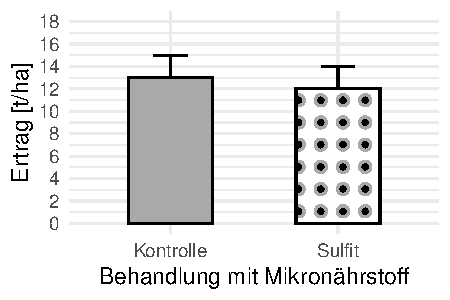
\includegraphics[width=\maxwidth]{img/mc-testing-ttest-02-1} 

}







\begin{enumerate}
\item [\textbf{A} \msquare] Die Barplots deuten auf keinen signifikanten Unterschied. Der Effekt liegt vermutlich bei -10 unter einer groben Abschätzung. Wir müssen aber eine ANOVA rechnen um den Effekt wirklich bestimmen zu können.
\item [\textbf{B} \msquare] Es liegt ein signifikanter Unterschied vor. Der Effekt liegt bei -1.
\item [\textbf{C} \msquare] Es liegt ein signifikanter Unterschied vor. Der Effekt liegt bei -10.
\item [\textbf{D} \msquare] Nach Betrachtung des Barplots liegt kein signifikanter Unterschied vor. Der Effekt kann nicht bei einem t-Test aus Barplots bestimmt werden.
\item [\textbf{E} \msquare] Nach Betrachtung des Barplots liegt kein signifikanter Unterschied vor. Der Effekt liegt bei -10.
\end{enumerate}

\section{Aufgabe \hfill (2 Punkte)}




In Ihrer Abschlussarbeit betrachten Sie die Effekte von einer Behandlung vor und nach der Gabe eines Vitamins. Sie müssen einen gepaarten t-Test rechnen. Welche Aussage ist richtig?



\begin{enumerate}
\item [\textbf{A} \msquare] Abhängige Beobachtungen müssen gesondert in einem gepaarten t-Test modelliert werden. Wenn wiederholt an dem gleichen Tier oder Pflanze gemessen wird, dann bilden wir den Quotienten zwischen den beiden Zeitpunkten. Auf den Quotienten rechnen wir den gepaarten t-Test.
\item [\textbf{B} \msquare] Der gepaarte t-Test nutzt die Varianz der Beobachtungen jeweils paarweise und bildet dafür eine verbundene Stichprobe. Dieser Datensatz $d$ dient dann zur Differenzbildung.
\item [\textbf{C} \msquare] Der gepaarte t-Test wird genutzt, wenn die Differenzen der Beobachtungen verbunden sind und wir dadurch die Unabhäängigkeit nicht mehr vorliegen haben.
\item [\textbf{D} \msquare] Der gepaarte t-Test wird gerechnet, wenn die Beobachtungen nicht unabhängig voneinander sind. Wir messen wiederholt an dem gleichen Probanden oder Tier oder Pflanze. Wir bilden die Differenzen um den gepaarten t-Test rechnen zu können.
\item [\textbf{E} \msquare] Wenn die Beobachtungen unabhängig voneinander sind, rechnen wir einen gepaarten t-Test. Messen wir wiederholt an dem gleichen Tier oder Pflanze dann bilden wir das Produkt zwischen den zwei Messpunkten.
\end{enumerate}

\section{Aufgabe \hfill (2 Punkte)}



In Ihrer Abschlussarbeit passen die Ergebnisse einer ANOVA und eines multiplen Vergleiches nicht zusammen. Nach einem Experiment mit vier Maissorten ergibt eine ANOVA ($p = 0.048$). Sie führen anschließend die paarweisen t-Tests für alle Vergleiche durch. Nach der Adjustierung für multiples Testen ist kein p-Wert unter der $\alpha$-Schwelle. Sie schauen sich auch die rohen, unadjustierten p-Werte an und finden hier als niedrigsten p-Wert $p_{3-2} = 0.052$. Welche Aussage ist richtig?




\begin{enumerate}
\item [\textbf{A} \msquare] Hier kommt der Effekt der stiegenden Fallzahl auf die Anzahl an signifikante Ergebnisse zu tragen. Da die ANOVA auf mehr Fallzahl testet als die einzelnen paarweisen t-Tests, kann die ANOVA leichter einen signifikanten Unterscheid nachweisen. Die p-Werte sind immer etwas kleiner als bei den t-Tests.
\item [\textbf{B} \msquare] Die adjustierten p-Werte deuten in die richtige Richtung. Zusammen mit den nicht signifikanten rohen p-Werten ist von einem Fehler in der ANOVA auszugehen.
\item [\textbf{C} \msquare] Das ist kein Wunder. Die ANOVA testet nicht auf der gesamten Fallzahl und die paarweisen t-Tests gewinnen immer eine oder mehr Gruppen als Fallzahl dazu. Mit steigender Fallzahl sind mehr signifikante Unterschiede zu erwarten. Die p-Werte unterscheiden sich numerisch auch kaum.
\item [\textbf{D} \msquare] Das Beispiel kann so nicht auftreten, da die ANOVA und die t-Tests algorithmisch miteinander verschränkt sind.
\item [\textbf{E} \msquare] Es gibt einen Fehler in der Varianzstruktur. Daher kann die ANOVA nicht richtig sein und paarweise t-Tests liefern das richtige Ergebnis.
\end{enumerate}
    
% -----------------------------------------------------------------------
\clearpage
% -----------------------------------------------------------------------
\part{Deskriptive Statistik \& Explorative Datenanalyse}
% -----------------------------------------------------------------------

\section{Aufgabe \hfill (8 Punkte)}

\textit{Geben Sie grundsätzlich Formeln und Rechenweg zur Lösung der Teilaufgaben mit an!} \\[1Ex]
 

 
%% --------------------------------------------------------------------
\begin{minipage}[t]{0.5\textwidth}

\includegraphics[width = 1.3cm]{/Users/kruppajo/work/GitHub/exam/avatare/Nilufar.png}
\end{minipage}
\begin{minipage}[t]{0.5\textwidth}
\hfill
\href{https://youtu.be/t0WYa_LVc5o}{
\includegraphics[width = 2cm]{img/youtube}}
\end{minipage}
\vspace{-3ex}
%% --------------------------------------------------------------------



\paragraph{Zerforschen des Barplots}

Barplots sind bedeutend in der Darstellung von wissenschaftlichen Ergebnissen. Leider hat sich Nilufar nicht gemerkt, welche statistischen Maßzahlen für einen Barplot erhoben werden müssen. Besser wäre was anderes gewesen. Nilufar liebt Hip Hop. Darin kann sie sich wirklich verlieren und immer wieder neu begeistern. Das ist in soweit doof, da nach ihrer Betreuer erstmal ein Barplot nachgebaut werden soll, bevor es mit ihrer Hausarbeit losgeht. Dann hat sie schonmal den \Rlogo Code vorliegen und nachher geht dann alles schneller. Na dann mal los. Nilufar schafft sich die nötige Stimmung. Nilufar streichelt liebevoll das Huhn. Der Kopf ist in ihrem Schloß vergraben um den Klang von Deichkind zu dämpfen. In der Behandlung für Erbsen werden verschiedene Lichtstufen ($none$, $200lm$ und $600lm$) sein. Erfasst wird als Endpunkt ($Y$) \textit{Trockengewicht}. Nilufar soll dann \textit{drymatter} in ihrer Exceldatei eintragen.



{\centering 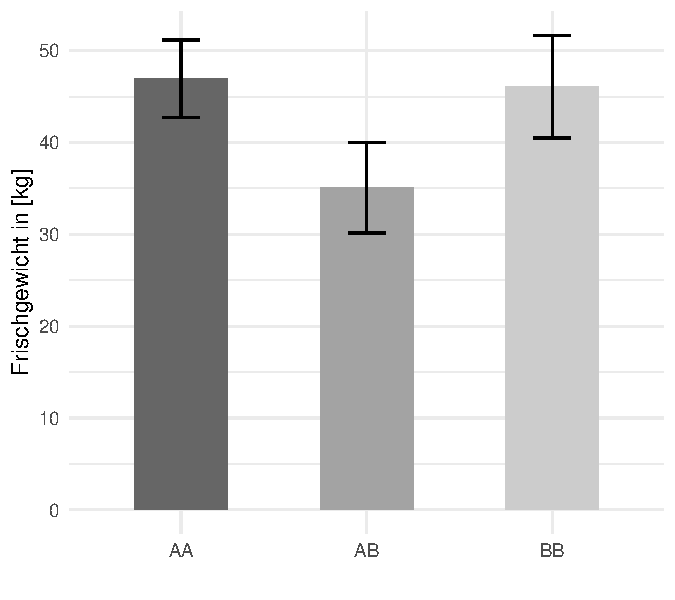
\includegraphics[width=\maxwidth]{img/barplot-02-1} 

}




Leider kennt sich Nilufar mit der Erstellung von Barplots in \Rlogo nicht aus. Deshalb braucht sie bei der Visualisierung Ihre Hilfe!

\begin{enumerate}
\item Formulieren Sie die wissenschaftliche Fragestellung! \textbf{(1 Punkt)}
\item Erstellen Sie eine Tabelle mit den statistischen Maßzahlen der drei Barplots! \textit{Beachten Sie die korrekte Darstellungsform der statistischen Maßzahlen!} \textbf{(3 Punkte)}
\item Erstellen Sie einen beispielhaften Datensatz im \Rlogo üblichen Format, aus dem die drei Barplots \textit{möglicherweise} erstellt wurden! \textbf{(2 Punkte)}
\item Kann Nilufar einen Unterschied zwischen den Behandlungen erwarten? Begründen Sie Ihre Antwort! \textbf{(2 Punkte)}
\end{enumerate} 
\clearpage
% -----------------------------------------------------------------------

\section{Aufgabe \hfill (8 Punkte)}

\textit{Geben Sie grundsätzlich Formeln und Rechenweg zur Lösung der Teilaufgaben mit an!} \\[1Ex]
 

 
%% --------------------------------------------------------------------
\begin{minipage}[t]{0.5\textwidth}

\includegraphics[width = 1.3cm]{/Users/kruppajo/work/GitHub/exam/avatare/Nilufar.png}
\end{minipage}
\begin{minipage}[t]{0.5\textwidth}
\hfill
\href{https://youtu.be/vXnLttRL_VI}{
\includegraphics[width = 2cm]{img/youtube}}
\end{minipage}
\vspace{-3ex}
%% --------------------------------------------------------------------



\paragraph{Visualisierung des Barplots}


Nilufar steht vor einem ersten Problem, denn wenn es nach ihrem Betreuer geht, soll sie in einem einem Feldexperiment Erbsen auswertet. Soweit eigentlich alles passend. Besser wäre was anderes gewesen. Am Ende dann doch besser Hip Hop. Wunderbar. Eine echte Ablenkung für Nilufar. Die Behandlung waren verschiedene Düngestufen ($ctrl$, $low$ und $high$). In ihrer Exceldatei hat sie den Endpunkt ($Y$) \textit{Ertrag} als \textit{yield} aufgenommen. Nun soll Nilufar die Daten eimal als Barplots in einer Präsentation visualisieren, damit ihrem Betreuer wieder klar wird, was sie eigentlich nochmal gemacht hat und was für ein Ergbnis in einem statistischen Test zu erwarten wäre. Wäre da nicht noch etwas. Eine echte Herausforderung für sie war schon immer die Erwartung gewesen. Ein leidiges Lied. Aber egal. Einfach mal raus um zu Kicken. Ohne Ziel und Uhr. Das ist was für Nilufar.

\begin{table}[!h]
\centering
\begin{tabular}{cc}
\toprule
treatment & yield\\
\midrule
ctrl & 29.2\\
high & 31.0\\
high & 29.0\\
low & 27.6\\
low & 28.7\\
\addlinespace
high & 31.8\\
low & 32.2\\
high & 29.6\\
ctrl & 42.3\\
high & 20.8\\
\addlinespace
low & 26.3\\
low & 36.5\\
ctrl & 30.0\\
\bottomrule
\end{tabular}
\end{table}



Leider kennt sich Nilufar mit der Erstellung von Barplots nicht aus. Deshalb braucht sie bei der Visualisierung Ihre Hilfe!

\begin{enumerate}
\item Formulieren Sie die wissenschaftliche Fragestellung! \textbf{(1 Punkt)}
\item Zeichnen Sie in \textit{einer} Abbildung die Barplots für die Behandlung von Erbsen! Beschriften Sie die Achsen entsprechend!\textbf{(4 Punkte)}
\item Beschriften Sie \textit{einen} Barplot mit den gängigen statistischen Maßzahlen! \textbf{(2 Punkte)}
\item Wenn Nilufar \textit{keinen Effekt} zwischen den Behandlungen von Erbsen erwarten würde, wie sehen dann die Barplots aus? \textit{Antworten Sie mit einer Skizze der Barplots!}
  \textbf{(1 Punkt)}
\end{enumerate} 
\clearpage
% -----------------------------------------------------------------------

\section{Aufgabe \hfill (9 Punkte)}

\textit{Geben Sie grundsätzlich Formeln und Rechenweg zur Lösung der Teilaufgaben mit an!} \\[1Ex]
 

 
%% --------------------------------------------------------------------
\begin{minipage}[t]{0.5\textwidth}

\includegraphics[width = 1.3cm]{/Users/kruppajo/work/GitHub/exam/avatare/Paula.png}
\end{minipage}
\begin{minipage}[t]{0.5\textwidth}
\hfill
\href{https://youtu.be/Xf0yE-o7bEU}{
\includegraphics[width = 2cm]{img/youtube}}
\end{minipage}
\vspace{-3ex}
%% --------------------------------------------------------------------



\paragraph{Zerforschen des Boxplots}

Paula und der Perfektionismus, eine unendliche Geschichte mit kniffeligen Wendungen. Deshalb gilt anschauen, was andere vor einem gemacht haben. Für Paula ist es eine Möglichkeit schneller ans Ziel zu gelangen. Paula soll in ihrer Hausarbeit Lauch untersuchen. Die Behandlung in ihrer Hausarbeit werden verschiedene Lichtstufen ($none$, $200lm$ und $600lm$) sein. Erheben wird Paula als Outcome ($Y$) \textit{Frischegewicht} benannt als \textit{freshmatter} in ihrer Exceldatei. Von ihrem Betreuer erhält sie nun folgende Abbildung von Boxplots, die sie erstmal zur Übung nachbauen soll, bevor sie mit dem eigentlichen Versuch beginnt. Aber nur in passender Atmospäre! Auf seinem Second Screen läuft Jagd auf roter Oktober und Paula schaufelt Smarties. Nicht effizient, aber gut.



{\centering 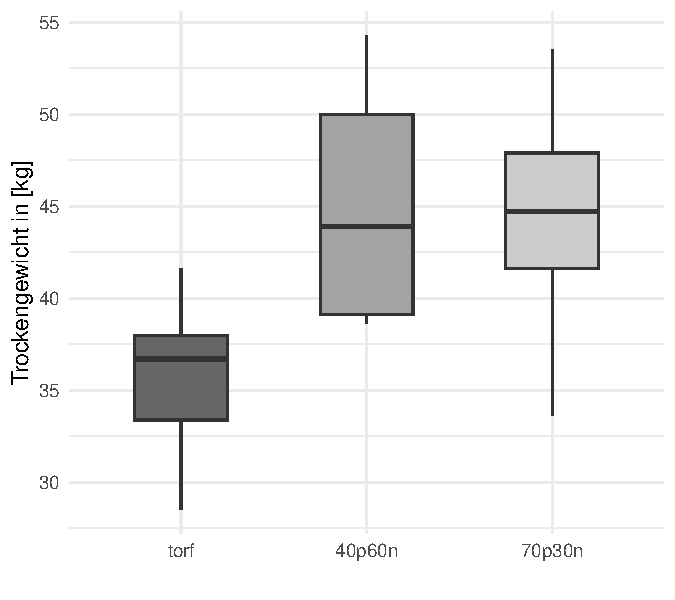
\includegraphics[width=\maxwidth]{img/boxplot-02-zer-1} 

}




Leider kennt sich Paula mit der Erstellung von Boxplots in \Rlogo nicht aus. Deshalb braucht sie bei der Visualisierung Ihre Hilfe!

\begin{enumerate}
\item Erstellen Sie eine Tabelle mit den statistischen Maßzahlen aus der obigen Abbildung der drei Boxplots! \textit{Beachten Sie die korrekte Darstellungsform der statistischen Maßzahlen!} \textbf{(3 Punkte)}
\item Beschriften Sie \textit{einen} der Boxplots mit den gängigen statistischen Maßzahlen! \textbf{(2 Punkte)}
\item Erstellen Sie einen beispielhaften Datensatz, aus dem die drei Boxplots \textit{möglicherweise} erstellt wurden, im \Rlogo üblichen Format! \textbf{(2 Punkte)}
\item Kann Paula einen Unterschied zwischen den Behandlungen erwarten? Begründen Sie Ihre Antwort! \textbf{(2 Punkte)}
\end{enumerate} 
\clearpage
% -----------------------------------------------------------------------

\section{Aufgabe \hfill (9 Punkte)}

\textit{Geben Sie grundsätzlich Formeln und Rechenweg zur Lösung der Teilaufgaben mit an!} \\[1Ex]
 

 
%% --------------------------------------------------------------------
\begin{minipage}[t]{0.5\textwidth}

\includegraphics[width = 1.3cm]{/Users/kruppajo/work/GitHub/exam/avatare/Paula.png}
\end{minipage}
\begin{minipage}[t]{0.5\textwidth}
\hfill
\href{https://youtu.be/0xc0jIPeiyw}{
\includegraphics[width = 2cm]{img/youtube}}
\end{minipage}
\vspace{-3ex}
%% --------------------------------------------------------------------



\paragraph{Visualisierung des Boxplots}

Paula und der Perfektionismus, eine unendliche Geschichte mit kniffeligen Wendungen. Deshalb gilt anschauen, was andere vor einem gemacht haben. Für Paula ist es eine Möglichkeit schneller ans Ziel zu gelangen. Deshalb hat sich Paula viele Poster in der Fakultät angeschaut und ist zum Schluß gekommen, dass Boxplots eine häufig genutzte Abbildung sind. Paula soll nun in ihrem Projektbericht Erdbeeren untersuchen. Die Behandlung in ihrem Projektbericht sind verschiedene Bewässerungstypen ($low$ und $high$). Erhoben wurden von Paula als Endpunkt ($Y$) \textit{Trockengewicht} benannt als \textit{drymatter} in ihrer Exceldatei. Erwartungsgemäß erhält sie von ihrer Betreuerin den Auftrag die erhobenen Daten als Boxplots darzustellen. Dann kann Paula auch schonmal abschätzen, was bei einem statistischen Test rauskommen könnte. Darüber hinaus kann Paula anhand Boxplots eine Aussage über die Normalverteilung von $Y$ treffen. Na dann mal los. Paula schafft sich die nötige Stimmung. Paula streichelt liebevoll die Ratte. Der Kopf ist in ihrem Schloß vergraben um den Klang von White Lies zu dämpfen.

\begin{table}[!h]
\centering
\begin{tabular}{cc}
\toprule
treatment & drymatter\\
\midrule
high & 27.4\\
low & 18.5\\
high & 31.6\\
low & 25.9\\
high & 20.2\\
\addlinespace
high & 27.2\\
high & 23.0\\
low & 30.3\\
low & 18.9\\
low & 29.8\\
\addlinespace
low & 31.6\\
low & 18.2\\
high & 31.1\\
low & 25.5\\
low & 32.1\\
\addlinespace
low & 17.3\\
high & 22.5\\
high & 29.4\\
high & 39.7\\
high & 35.2\\
\bottomrule
\end{tabular}
\end{table}



Leider kennt sich Paula mit der Erstellung von Boxplots nicht aus. Deshalb braucht sie bei der Visualisierung Ihre Hilfe!

\begin{enumerate}
\item Zeichnen Sie in \textit{einer} Abbildung die beiden Boxplots für die zwei Behandlungen von Erdbeeren! Beschriften Sie die Achsen entsprechend! \textbf{(5 Punkte)} 
\item Wie ist Ihr Vorgehen, wenn Sie eine \textit{gerade} Anzahl an
  Beobachtungen pro Gruppe haben? \textbf{(1 Punkt)}
\item Beschriften Sie \textit{einen} der beiden Boxplots mit den gängigen
  statistischen Maßzahlen! \textbf{(2 Punkte)}
\item Wenn Sie \textit{keinen Effekt} zwischen den Behandlungen von
  Erdbeeren erwarten würden, wie sehen dann die beiden Boxplots aus?
  \textit{Antworten Sie mit einer Skizze der Boxplots!}
  \textbf{(1 Punkt)}
\end{enumerate} 
\clearpage
% -----------------------------------------------------------------------

\section{Aufgabe \hfill (8 Punkte)}

\textit{Geben Sie grundsätzlich Formeln und Rechenweg zur Lösung der Teilaufgaben mit an!} \\[1Ex]
 

 
%% --------------------------------------------------------------------
\begin{minipage}[t]{0.5\textwidth}

\includegraphics[width = 1.3cm]{/Users/kruppajo/work/GitHub/exam/avatare/Yuki.png}
\end{minipage}
\begin{minipage}[t]{0.5\textwidth}
\hfill
\href{https://youtu.be/aXvxGC4YLqk}{
\includegraphics[width = 2cm]{img/youtube}}
\end{minipage}
\vspace{-3ex}
%% --------------------------------------------------------------------



\paragraph{Visualisierung des Histogramm für kategoriale Daten}

In seiner Hausarbeit möchte Yuki gerne die Daten aus einem Kreuzungsexperiment mit Schweinen in einem Histogramm darstellen. Das Histogramm erlaubt ihm dabei Rückschlüsse auf die Verteilung über das Outcome ($Y$) zu treffen. Yuki schmeißt noch eine Handvoll Reese's Peanut Butter Cups in seinen Rachen. Im Hintergrund klirrt leise der Spiegel zum Sound von London Grammar. In seinem Experiment hat Yuki die Anzahl an gedrehten Haaren/Federn pro $cm^2$ gezählt. Es wäre einfacher, wenn da nicht noch was wäre. Eine echte Herausforderung für ihn war schon immer die Faulheit gewesen. Ein leidiges Lied. Wenn London Grammar ertönt, dann sucht das Minischwein schleunigst Schutz unter dem Sofa. Yuki schüttelt den Kopf.

\begin{center}
Die Anzahl an gedrehten Haaren/Federn pro $cm^2$: 4, 4, 6, 5, 8, 3, 5, 2, 6, 6, 3, 5, 5, 0, 2, 6, 3, 8, 7, 3, 5, 2, 6, 3, 5, 5, 8, 5, 8, 3, 6, 3, 6
\end{center}

Leider kennt sich Yuki mit der Erstellung von Histogrammen überhaupt nicht aus. Deshalb braucht er bei der Erstellung Ihre Hilfe!

\begin{enumerate}
\item Zeichen Sie ein Histogramm um die Verteilung der Daten zu visualisieren! (\textbf{3 Punkte})
\item Beschriften Sie die Achsen der Abbildung! (\textbf{2 Punkte})
\item Ergänzen Sie die absoluten und relativen Häufigkeiten in der
  Abbildung! \textbf{(1 Punkt)}
\item Berechnen Sie aus den Daten die \textit{Wahrscheinlichkeit}
  gleich oder mehr als die Anzahl 4 zu beobachten! \textbf{(1
    Punkt)}
\item Berechnen Sie aus den Daten die \textit{Chance} gleich oder mehr
  als die Anzahl 4 zu beobachten! \textbf{(1 Punkt)}
\end{enumerate}

 
\clearpage
% -----------------------------------------------------------------------

\section{Aufgabe \hfill (8 Punkte)}

\textit{Geben Sie grundsätzlich Formeln und Rechenweg zur Lösung der Teilaufgaben mit an!} \\[1Ex]
 

 
%% --------------------------------------------------------------------
\begin{minipage}[t]{0.5\textwidth}

\includegraphics[width = 1.3cm]{/Users/kruppajo/work/GitHub/exam/avatare/Mark.png}
\end{minipage}
\begin{minipage}[t]{0.5\textwidth}
\hfill
\href{https://youtu.be/ORHSPTCdfeY}{
\includegraphics[width = 2cm]{img/youtube}}
\end{minipage}
\vspace{-3ex}
%% --------------------------------------------------------------------



\paragraph{Visualisierung des Histogramm für kontinuierliche Daten}

In seiner Hausarbeit möchte Mark gerne die Daten aus einem Kreuzungsexperiment mit Schweinen in einem Histogramm darstellen. Das Histogramm erlaubt ihm dabei Rückschlüsse auf die Verteilung über das Outcome ($Y$) zu treffen 'Hm...', Marzipankugeln und Andrea Berg. Das ist und bleibt die beste Kombination zum Nachdenken für Mark. In seinem Experiment hat Mark die mittlere Anzahl an weißen Blutkörperchen gezählt. Es wäre einfacher, wenn da nicht noch was wäre. Mark und die Unsicherheit, eine unendliche Geschichte mit kniffeligen Wendungen. Wenn Andrea Berg ertönt, dann sucht der Hamster schleunigst Schutz unter dem Sofa. Mark schüttelt den Kopf.

\begin{center}
Die mittlere Anzahl an weißen Blutkörperchen: 10.2, 7.6, 9.7, 12.3, 7.9, 12.2, 11.2, 10.9, 11.8, 5.9, 11.3, 8.9, 9.2, 8.7, 10.7, 12, 8.1, 11.7, 8.3, 9.2, 6.1, 9
\end{center}

Leider kennt sich Mark mit der Erstellung von Histogrammen überhaupt nicht aus. Deshalb braucht er bei der Erstellung Ihre Hilfe!

\begin{enumerate}
\item Zeichen Sie ein Histogramm um die Verteilung der Daten zu visualisieren! (\textbf{3 Punkte})
 \item Erläutern Sie Ihr Vorgehen um ein Histogramm für kontinuierliche Daten zu zeichnen!  (\textbf{2 Punkte})
\item Beschriften Sie die Achsen der Abbildung! (\textbf{2 Punkte})
\item Ergänzen Sie die relativen Häufigkeiten in der Abbildung! \textbf{(1 Punkt)}  
\end{enumerate}

 
\clearpage
% -----------------------------------------------------------------------

\section{Aufgabe \hfill (10 Punkte)}

\textit{Geben Sie grundsätzlich Formeln und Rechenweg zur Lösung der Teilaufgaben mit an!} \\[1Ex]
 

 
%% --------------------------------------------------------------------
\begin{minipage}[t]{0.5\textwidth}

\includegraphics[width = 1.3cm]{/Users/kruppajo/work/GitHub/exam/avatare/Alex.png}
\end{minipage}
\begin{minipage}[t]{0.5\textwidth}
\hfill
\href{https://youtu.be/VAqiUdV4WQ0}{
\includegraphics[width = 2cm]{img/youtube}}
\end{minipage}
\vspace{-3ex}
%% --------------------------------------------------------------------




\paragraph{Visualisierung des Scatterplots}

Wenn es nach Alex ginge, wäre er schon längst fertig mit seiner Hausarbeit. Geht es aber nicht. Aus den Boxen wummert Abba und sein Mund ist verklebt von Gummibärchen. 'Herrlich', denkt Alex. In seiner Hausarbeit hatte er ein Feldexperiment im Oldenburger Land durchgeführt. Nach der Meinung seinem Betreuer sieht das jedoch etwas anders aus. Jetzt soll er doch noch eine explorative Datenanalyse für den Zusammenhang zwischen durschnittlichen Niederschlag [ml/w] und Trockengewicht [kg/ha] in Lauch durchführen. Wie nervig! Wenn die Gefälligkeit nicht wäre, ja dann wäre wohl vieles möglich für Alex! Aber so.. Da zwei kontinuierliche Variablen vorliegen, geht die explorative Datenanalyse leider nicht mit Boxplots oder Barplots. Dann was anderes. Wenn Alien läuft, dann ist die Katze nicht mehr da. Aber jetzt braucht er mal Entspannung!

\begin{table}[!h]
\centering
\begin{tabular}{cc}
\toprule
Trockengewicht [kg/ha] & Durschnittlichen Niederschlag [ml/w]\\
\midrule
24.8 & 33.2\\
13.8 & 22.1\\
18.6 & 31.6\\
20.5 & 33.9\\
21.0 & 30.5\\
\addlinespace
17.0 & 27.9\\
13.5 & 26.5\\
20.2 & 26.6\\
28.5 & 41.6\\
\bottomrule
\end{tabular}
\end{table}



Leider kennt sich Alex mit der Erstellung einer explorativen Datenanalyse für kontinuierliche Daten überhaupt nicht aus. Deshalb braucht er bei der Erstellung Ihre Hilfe!

\begin{enumerate}
\item Erstellen Sie eine Visualisierung für die Datentabelle. Beschriften Sie
  die Achsen entsprechend! \textbf{(4 Punkte)}
\item Schätzen Sie eine Gerade durch die Punkte! \textbf{(1 Punkt)}
\item Beschriften Sie die Gerade mit den gängigen statistischen Maßzahlen! Geben Sie die numerischen Zahlenwerte mit an! \textbf{(3 Punkte)}
\item Wenn \textit{ein} Effekt von $x$ auf $y$ vorhanden wäre, wie würde die Gerade verlaufen und welche Werte würden die statistischen Maßzahlen annehmen? \textbf{(2 Punkt)}
\end{enumerate} 
\clearpage
% -----------------------------------------------------------------------

\section{Aufgabe \hfill (10 Punkte)}

\textit{Geben Sie grundsätzlich Formeln und Rechenweg zur Lösung der Teilaufgaben mit an!} \\[1Ex]
 

 
%% --------------------------------------------------------------------
\begin{minipage}[t]{0.5\textwidth}

\includegraphics[width = 1.3cm]{/Users/kruppajo/work/GitHub/exam/avatare/Alex.png}
\end{minipage}
\begin{minipage}[t]{0.5\textwidth}
\hfill
\href{https://youtu.be/t_1KL77mfmg}{
\includegraphics[width = 2cm]{img/youtube}}
\end{minipage}
\vspace{-3ex}
%% --------------------------------------------------------------------



\paragraph{Visualisierung des Mosaicplots}

Das Verrückte ist, dass die Katze Alien wirklich liebt. Das ist Alex sehr recht, denn er braucht Entspannung. Aber Ablenkung hilft nur begrenzt. 'Uff!', denkt sich Alex. Jetzt hat er doch tatsächlich zwei kategoriale Variablen in seinem Projektbericht gemessen. Zum einen die Behandlung Klimakontrolle [ja/nein] und zum anderen die Messung Protein/Fettrate im Zielbereich [ja/nein] im Kontext von Puten. Hierfür hat er ein Kreuzungsexperiment im Wendland durchgeführt. Jetzt möchte Alex die Daten einmal in einer explorativen Datenanalyse darstellen. Danach kann er dann über den passenden statistischen Test nachdenken. Dabei unterstützt seine Betreuerin diesen Ansatz bevor es in der Datenanalyse weiter geht. So schön wie so gut. Wenn die Gefälligkeit nicht wäre, ja dann wäre wohl vieles möglich für Alex! Aber so..



\vspace{1Ex}

\begin{center}
\begin{minipage}[t]{0.45\textwidth}
%\small
\begin{center}

\begin{tabular}{p{2.5cm}p{2.5cm}p{2.5cm}p{2.5cm}}
\toprule
Protein/Fettrate im Zielbereich & Klimakontrolle\\
\midrule
ja & ja\\
nein & ja\\
ja & nein\\
ja & ja\\
nein & ja\\
\addlinespace
nein & nein\\
ja & nein\\
nein & ja\\
nein & ja\\
nein & ja\\
\addlinespace
nein & nein\\
ja & ja\\
ja & nein\\
ja & nein\\
ja & nein\\
\addlinespace
ja & ja\\
\bottomrule
\end{tabular}


\end{center}
\end{minipage}
\begin{minipage}[t]{0.45\textwidth}
%\small
\begin{center}

\begin{tabular}{p{2.5cm}p{2.5cm}p{2.5cm}p{2.5cm}}
\toprule
Protein/Fettrate im Zielbereich & Klimakontrolle\\
\midrule
ja & nein\\
ja & nein\\
ja & ja\\
nein & nein\\
nein & ja\\
\addlinespace
nein & nein\\
nein & nein\\
nein & nein\\
ja & ja\\
ja & nein\\
\addlinespace
nein & ja\\
nein & ja\\
nein & ja\\
nein & ja\\
ja & nein\\
\addlinespace
ja & nein\\
\bottomrule
\end{tabular}


\end{center}
\end{minipage}
\end{center}

\vspace{2Ex}

Leider kennt sich Alex mit der Erstellung einer explorativen Datenanalyse für kategoriale Daten überhaupt nicht aus. Deshalb braucht er bei der Erstellung Ihre Hilfe!

\begin{enumerate}
\item Stellen Sie den Zusammenhang zwischen den beiden kategorialen Variablen in einer zusammenfassenden Tabelle dar! \textbf{(3 Punkte)}
\item Visualisieren Sie den Zusammenhang zwischen den beiden kategorialen Variablen! \textbf{(3 Punkte)}
\item Berechnen Sie die Verhältnisse in der Visualisierung! Welche Annahme haben Sie getroffen? \textbf{(2 Punkte)}
\item Wenn \textit{ein} Effekt von der Behandlung vorliegen würde, wie würde die Tabelle und die Visualisierung aussehen? \textbf{(2 Punkt)}
\end{enumerate} 
\clearpage
% -----------------------------------------------------------------------

\section{Aufgabe \hfill (10 Punkte)}

\textit{Geben Sie grundsätzlich Formeln und Rechenweg zur Lösung der Teilaufgaben mit an!} \\[1Ex]
 

 
%% --------------------------------------------------------------------
\begin{minipage}[t]{0.5\textwidth}

\includegraphics[width = 1.3cm]{/Users/kruppajo/work/GitHub/exam/avatare/Jessica.png}\hspace{-4mm}
\includegraphics[width = 1.3cm]{/Users/kruppajo/work/GitHub/exam/avatare/Paula.png}
\end{minipage}
\begin{minipage}[t]{0.5\textwidth}
\hfill
\href{https://youtu.be/Op-gjzASH9I}{
\includegraphics[width = 2cm]{img/youtube}}
\end{minipage}
%% --------------------------------------------------------------------



\paragraph{Visualisierung von Verteilungen}

'Was hast du dir denn da hingeklebt? \textit{Frei ist, wer missfallen kann.}\footnote{Oschmann, A. (2024) Mädchen stärken: Stärken fördern, Selbstwert erhöhen und liebevoll durch Krisen begleiten. Goldegg Verlag}', liest Paula vom Kühlschrank vor. Paula und Jessica sitzen zusammen in der Küche und versuchen zu verhindern, dass die Ratte den Biomüll mampft. 'Können wir uns auf die etwas kryptische Aufgabe konzentrieren?', nöhlt Jessica. Die beiden schauen angestrengt auf die drei Boxplots. Das Ziel ist es zu verstehen, wie eine Verteilung anhand eines Boxplots bewertet werden kann. Jessica und der Mangel machen die Sache nicht einfacher.



{\centering 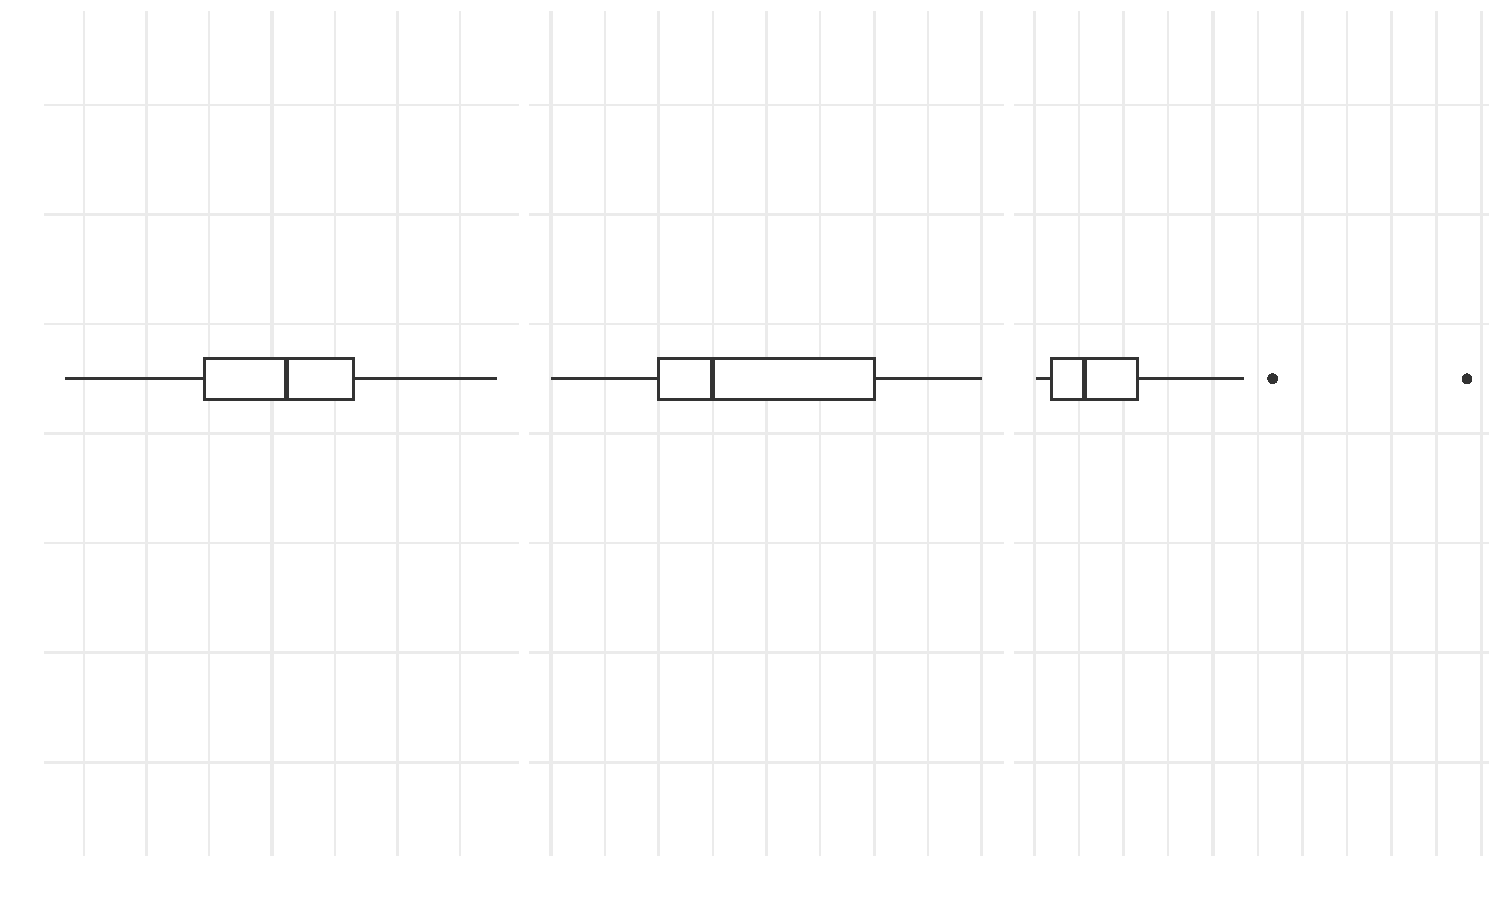
\includegraphics[width=\maxwidth]{img/desc-stat-11-1} 

}




Jetzt brauchen Paula und Jessica Ihre Hilfe bei der Abschätzung einer Verteilung anhand von Boxplots um ihre Arbeit dann in diesem Semester noch abschließen zu können.

\begin{enumerate}
\item Zeichnen Sie über die Boxplots die entsprechende zugehörige Verteilung! \textbf{(3 Punkte)} 
\item Zeichnen Sie unter die Boxplots die entsprechende zugehörige Beobachtungen als Stiche! \textbf{(3 Punkte)}
\item Wie viel Prozent der Beobachtungen fallen in das IQR? Ergänzen Sie die Abbildung entsprechend um den Bereich! \textbf{(2 Punkte)}
\item Wie viel Prozent der Beobachtungen fallen in $\bar{y} \pm 1s$ und $\bar{y} \pm 2s$  unter der Annahme einer Normalverteilung? \textbf{(2 Punkte)}
\end{enumerate} 
\clearpage
% -----------------------------------------------------------------------

\section{Aufgabe \hfill (10 Punkte)}

\textit{Geben Sie grundsätzlich Formeln und Rechenweg zur Lösung der Teilaufgaben mit an!} \\[1Ex]
 

 
%% --------------------------------------------------------------------
\begin{minipage}[t]{0.5\textwidth}

\includegraphics[width = 1.3cm]{/Users/kruppajo/work/GitHub/exam/avatare/Nilufar.png}\hspace{-4mm}
\includegraphics[width = 1.3cm]{/Users/kruppajo/work/GitHub/exam/avatare/Steffen.png}
\end{minipage}
\begin{minipage}[t]{0.5\textwidth}
\hfill
\href{https://youtu.be/ZrJhn2wPbq4}{
\includegraphics[width = 2cm]{img/youtube}}
\end{minipage}
%% --------------------------------------------------------------------



\paragraph{Visualisierung der Normalverteilung}

'Hmpf, wir sollen Normalverteilungen visualisieren. Waren das nicht so komische Glockenkurven?', fragt sich Nilufar. Steffen hat Oreos mitgebracht und Taylor Swift aufgedreht. Immerhin etwas. Jetzt sollen die beiden diese Aufgabe zur Normalverteilung lösen. Es geht um verschiedene Normalverteilungen udn zu verstehen, wie die Parameter der Normalverteilung funktionieren. Anscheinend hängen Normalverteilungen vom Mittelwert $\bar{y}$ und der Standardabweichung $s$ ab. 'Wozu brauchen wir nochmal Normalverteilungen?', entfährt es Steffen. Durch das Mampfen von Takis Blue Heat durch Nilufar versteht er kein Wort der Antwort. \\



Jetzt brauchen Steffen und Nilufar Ihre Hilfe bei der Abschätzung einer Verteilung um ihre Arbeit dann in diesem Semester noch abschließen zu können.

\begin{enumerate}
\item Skizzieren Sie vier Normalverteilungen mit $\bar{y}_1 \neq \bar{y}_2 \neq \bar{y}_3 \neq \bar{y}_4$ und $s_1 = s_2 = s_3 = s_4$! \textbf{(3 Punkte)}
\item Beschriften Sie die Normalverteilungen mit den statistischen Maßzahlen! \textbf{(2 Punkte)}
\item Liegt Varianzhomogenität oder Varianzheterogenität vor? Begründen Sie Ihre Antwort! \textbf{(2 Punkte)}
\item In welchen Bereich fallen 68\% bzw. 95\% der Beobachtungen in einer Normalverteilung? Ergänzen Sie die Bereiche in \underline{einer} Normalverteilung! \textbf{(2 Punkte)}
\item Ergänzen Sie unter \underline{einer} der Normalverteilungen den entsprechenden Boxplot! \textbf{(1 Punkt)}
\end{enumerate}

 
\clearpage
% -----------------------------------------------------------------------

\section{Aufgabe \hfill (10 Punkte)}

\textit{Geben Sie grundsätzlich Formeln und Rechenweg zur Lösung der Teilaufgaben mit an!} \\[1Ex]
 

 
%% --------------------------------------------------------------------
\begin{minipage}[t]{0.5\textwidth}

\includegraphics[width = 1.3cm]{/Users/kruppajo/work/GitHub/exam/avatare/Jessica.png}\hspace{-4mm}\includegraphics[width = 1.3cm]{/Users/kruppajo/work/GitHub/exam/avatare/Nilufar.png}
\end{minipage}
\begin{minipage}[t]{0.5\textwidth}
\hfill
\href{https://youtu.be/MiD42k4l5Ag}{\includegraphics[width = 2cm]{img/youtube}}
\end{minipage}
%% --------------------------------------------------------------------



\paragraph{Visualisierung der Normalverteilung und der Poissonverteilung}

'Wer hat sich denn sowas ausgedacht? Verteilungen?', entfährt es Nilufar und schaut dabei Jessica an. In ihrer Hand zerdrückt sie Schokobons von Jessica. 'Wir sollen eine Normalverteilung mit einem Mittelwert von $\bar{y}_1 = 3$ und einer Standardabweichung von $s_1 = 1$ zeichnen. Sowie eine weitere Normalverteilung mit einem Mittelwert von $\bar{y}_2 = 4$ und einer Standardabweichung von $s_2 = 1$. Keine Ahnung wie das geht. Darunter sollen dann noch eine Poissonverteilung mit einem Mittelwert von $\lambda_1 = 25$ sowie einer weiteren Poissonverteilung mit einem Mittelwert von $\lambda_2 = 3$ gezeichnet werden.', meint Jessica sichtlich eingeschüchtert und rettet noch ein paar Schokobons in seinem Mund. Nilufar und die Erwartung machen die Suche nach der Lösung nicht einfacher. Im Hintergrund spielt viel zu laut David Bowie, die diesmal Nilufar ausgewählt hat und das Huhn schon in die Küche vertrieben hat, wo es den Biomüll mampft.\\




{\centering \includegraphics[width=\maxwidth]{img/histogram-01-1} 

}




Jetzt brauchen Nilufar und Jessica Ihre Hilfe bei der Abschätzung einer Verteilung um ihre Arbeit dann in diesem Semester noch abschließen zu können.


\begin{enumerate}
\item Skizzieren Sie die zwei Normalverteilungen und zwei Poissonverteilungen! \textbf{(4 Punkte)}
\item Achten Sie auf die entsprechende Skalierung in den jeweiligen Abbildungen! \textbf{(2 Punkte)}
\item Ergänzen Sie unter \underline{einer} Normalverteilung den entsprechenden Boxplot! \textbf{(1 Punkt)}
\item Ergänzen Sie unter \underline{einer} Poissonverteilung den entsprechenden Boxplot! \textbf{(1 Punkt)}
\item Geben Sie ein Beispiel für ein Outcome $y$, welches einer Normalverteilung folgt! \textbf{(1 Punkt)}
\item Geben Sie ein Beispiel für ein Outcome $y$, welches einer Poissonverteilung folgt! \textbf{(1 Punkt)}
\end{enumerate} 
\clearpage
% -----------------------------------------------------------------------
\part{Statistisches Testen \& statistische Testtheorie}
% -----------------------------------------------------------------------  

\section{Aufgabe \hfill (9 Punkte)}


 
%% --------------------------------------------------------------------
\begin{minipage}[t]{0.5\textwidth}
\includegraphics[width = 1.3cm]{/Users/kruppajo/work/GitHub/exam/avatare/Jessica.png}\hspace{-4mm}\includegraphics[width = 1.3cm]{/Users/kruppajo/work/GitHub/exam/avatare/Jonas.png}
\end{minipage}
\begin{minipage}[t]{0.5\textwidth}
\hfill
\href{https://youtu.be/aHVYuFKTqZs}{\includegraphics[width = 2cm]{img/youtube}}
\end{minipage}
%% --------------------------------------------------------------------



\paragraph{Grundgesamtheit und experimentelle Stichprobe}

An einem schwülem Sommernachmittag sitzen Jessica und Jonas in einem Eiskaffee und wollen sich auf die Klausur vorbereiten. In fast allen Fragen geht es ja um die Interpretation eines statistischen Tests. Daher wollen die beiden jetzt nochmal nacharbeiten, was die Grundlagen der Stichprobe (eng. \textit{sample}) und der Grundgesamtheit (eng. \textit{population} oder \textit{ground truth}) sind. Jessica hat sich Schokobons Eisbecher bestellt und Jonas bleibt lieber bei einem Snickers Eis. 'Irre, was die Lebensmittelindustrie alles auf die Beine kriegt', merk Jonas an und Jessica schüttelt anerkennend den Kopf.

\vspace{1ex}

Leider kennen sich Jessica und Jonas mit der Grundgesamtheit und der Stuchprobe überhaupt nicht aus. Daher sind Sie gefragt!

\begin{enumerate}
\item Nennen Sie das statistische Verfahren und zwei konkrete Beispiele zur Durchführung um von einer Grundgesamtheit auf eine Stichprobe zu gelangen! \textbf{(3 Punkte)}
\item Erklären Sie den Zusammenhang zwischen Stichprobe und Grundgesamtheit an einem Schaubild! Beschriften Sie das Schaubild entsprechend!
  \textit{Nutzen Sie hierfür als Veranschaulichung die Körpergröße von Männern oder Frauen aus den Gummibärchendaten!}  \textbf{(3 Punkte)}
\item Erweitern Sie das Schaubild um die Entstehung von $Pr(D|H_0)$! \textit{Nutzen Sie hierfür als Veranschaulichung zusätzlich die Gruppierungsvariable "`Modul"' aus den Gummibärchendaten!}  \textbf{(3 Punkte)}
\end{enumerate} 
\clearpage
% -----------------------------------------------------------------------

\section{Aufgabe \hfill (9 Punkte)}


 
%% --------------------------------------------------------------------
\begin{minipage}[t]{0.5\textwidth}
\includegraphics[width = 1.3cm]{/Users/kruppajo/work/GitHub/exam/avatare/Nilufar.png}\hspace{-4mm}\includegraphics[width = 1.3cm]{/Users/kruppajo/work/GitHub/exam/avatare/Steffen.png}
\end{minipage}
\begin{minipage}[t]{0.5\textwidth}
\hfill
\href{https://youtu.be/Ric8ne39DtI}{\includegraphics[width = 2cm]{img/youtube}}
\end{minipage}
%% --------------------------------------------------------------------



\paragraph{Das Nullritual - Die statistische Testtheorie}

'Star Trek ist der beste Film, den es gibt.', meint Nilufar. Steffen entgegnet, ' Ich empfehle ja immer allen Harry Potter.'Die beiden sind im Zoo und diskutieren, ob Pinguine Knie haben. Eigentlich wollten beide nochmal die statistische Testheorie durchgehen, sind dann aber auf abenteuerlichen Wege im Zoo gelandet. Nilufar starrt wie hypnotisiert auf einen strullenden Elefanten und stopt die Zeit.\footnote{Yang, P. J., et al. (2014). Duration of urination does not change with body size. Proceedings of the National Academy of Sciences, 111(33), 11932-11937.} 'Du bist so peinlich.', entfährt es Steffen und schmeißt sich noch ein paar überteuerte Oreos rein.

\vspace{1ex}

Leider kennen sich Nilufar und Steffen mit statistischen Testtheorie, auch Null-Ritual genannt, überhaupt nicht aus. Geschweige denn mit der Visualisierung als Kreuztabelle.  

\begin{enumerate}
\item Tragen Sie folgende statistische Fachbegriffe zur statistischen Testtheorie korrekt eine selbst erstellte Kreuztabelle ein! \textbf{(3 Punkte)}
  \begin{center}
  \begin{tabular}{cccc}
  Testentscheidung & Richtige Entscheidung & H$_0$ beibehalten & $\beta$-Fehler \\
  \end{tabular}
  \end{center}
\item Ergänzen Sie Ihre erstellte Kreuztabelle um vier weitere, passende Fachbegriffe zur statistischen Testtheorie! \textbf{(2 Punkte)}
\end{enumerate}

Die Entscheidungsfindung durch einen statistischen Test kann auch durch die Analogie zu einem Feuermelder abgebildet werden. Dabei symbolisiert der Feuermelder den statistischen Test und es soll getestet werden, ob ein Feuer ausgebrochen ist.

\begin{enumerate}
  \setcounter{enumi}{2}    
\item In der Analogie des Feuermelders, wie lautet der $\alpha$-Fehler? \textbf{(1 Punkt)}
\item In der Analogie des Feuermelders, wie lautet der $\beta$-Fehler? \textbf{(1 Punkt)}
\item Wenn der Feuermelder einmal pro Tag messen würde, wie oft würde der Feuermelder mit einem $\alpha$ von 5\% in einem Jahr Alarm schlagen? Begründen Sie Ihre Antwort! \textbf{(2 Punkte)}
\end{enumerate}



 
\clearpage
% -----------------------------------------------------------------------

\section{Aufgabe \hfill (9 Punkte)}

\textit{Geben Sie grundsätzlich Formeln und Rechenweg zur Lösung der Teilaufgaben mit an!} \\[1Ex]


 
%% --------------------------------------------------------------------
\begin{minipage}[t]{0.5\textwidth}
\includegraphics[width = 1.3cm]{/Users/kruppajo/work/GitHub/exam/avatare/Mark.png}\hspace{-4mm}\includegraphics[width = 1.3cm]{/Users/kruppajo/work/GitHub/exam/avatare/Nilufar.png}
\end{minipage}
\begin{minipage}[t]{0.5\textwidth}
\hfill
\href{https://youtu.be/32JjH1eyuTU}{\includegraphics[width = 2cm]{img/youtube}}
\end{minipage}
%% --------------------------------------------------------------------



\paragraph{Visualisierung der Teststatistik $\boldsymbol{T_D}$ und dem p-Wert}

'Wir sollen die Teststatistik $T_D$ umd dem p-Wert visualisieren, da mit einer Visualisierung vieles verständlicher wird!', ruft Mark um Andrea Berg zu übertönen. 'Ich weiß nicht, was das jetzt helfen soll. Können wir nicht einfach schauen, ob der p-Wert kleiner als das Signifikanzniveau  $\alpha$ gleich 5\% ist? Und gut ist?', merkt Nilufar an, was aber im Refrain von Andrea Berg untergeht. Mark nickt im Beat. 'Wir haben hier eine t-verteilung unter der Annahme der Nullhypothese!', singt er.

\vspace{1ex}

Leider kennen sich Mark und Nilufar mit der Visualisierung der Teststatistik $T_D$ und dem p-Wert überhaupt nicht aus und brauchen dahr Ihre Hilfe!

\vspace{1ex}

\textit{Beachten Sie, dass im Folgenden \underline{keine numerisch korrekte Darstellung} verlangt wird! Es gilt Erkennbarkeit vor Genauigkeit!}

\begin{enumerate}
\item Ergänzen Sie eine beschriftete $x$-Achse! \textbf{(1 Punkt)}
\item Ergänzen Sie "`$\bar{y}_1 = \bar{y}_2$"'! \textbf{(1 Punkt)} 
\item Ergänzen Sie "`$A = 0.95$"'! \textbf{(1 Punkt)}
\item Zeichnen Sie $T_{\alpha=5\%}$ in die Abbildung! \textbf{(1 Punkt)} 
\item Zeichnen Sie das Signifikanzniveau $\alpha$ in die Abbildung! Begründen Sie Ihre Antwort! \textbf{(2 Punkte)} 
\item Zeichnen Sie $+T_{D}$ in die Abbildung! \textbf{(1 Punkt)}
\item Zeichnen Sie einen signifikant p-Wert in die Abbildung! Begründen Sie Ihre Antwort! \textbf{(2 Punkte)}   
\end{enumerate}



{\centering \includegraphics[width=\maxwidth]{img/statistisches-testen-3-1} 

}


 
\clearpage
% -----------------------------------------------------------------------

\section{Aufgabe \hfill (10 Punkte)}


 
%% --------------------------------------------------------------------
\begin{minipage}[t]{0.5\textwidth}
\includegraphics[width = 1.3cm]{/Users/kruppajo/work/GitHub/exam/avatare/Mark.png}\hspace{-4mm}\includegraphics[width = 1.3cm]{/Users/kruppajo/work/GitHub/exam/avatare/Steffen.png}
\end{minipage}
\begin{minipage}[t]{0.5\textwidth}
\hfill
\href{https://youtu.be/CN_O4fYPbhs}{\includegraphics[width = 2cm]{img/youtube}}
\end{minipage}
%% --------------------------------------------------------------------



\paragraph{Visualisierung des 95\% Konfidenzintervalls}

'So, was haben wir gemacht? Wir haben einen t-test für den Vergleich der Mittelwerte gerechnet.', meint Steffen. Mark schaut fragend. 'Hatten wir nicht alles zu einer Kontrolle verglichen? Das war doch so!', ruft Mark laut aus. 'Wir haben doch Messwert \textit{Chlorophyllgehalt nach Subsitution} erhoben.', stellt Steffen fest. Jetzt haben beide das Problem, die möglichen 95\% Konfidenzintervalle zu interpretieren.

\vspace{1ex}

Leider kennen sich Steffen und Mark mit der Visualisierung des 95\% Konfidenzintervall überhaupt nicht aus. 

\begin{enumerate}
\item Beschriften Sie die untenstehende Abbildung mit der Signifikanzschwelle! Begründen Sie Ihre Antwort! \textbf{(2 Punkte)}
\item Ergänzen Sie eine \textit{in den Kontext passende} Relevanzschwelle! Begründen Sie Ihre Antwort! \textbf{(2 Punkte)} 
\item Skizieren Sie in die untenstehende Abbildung sechs einzelne Konfidenzintervalle (a-f) mit den
  jeweiligen Eigenschaften! \textbf{(6 Punkte)}
  \begin{itemize}
  \item[(a)] Ein nicht signifikantes, nicht relevantes 95\% Konfidenzintervall 	
  \item[(b)] Ein 95\% Konfidenzintervall mit niedriger Varianz $s_p$ in der Stichprobe als der Rest 95\% der Konfidenzintervalle 	
  \item[(c)] Ein 95\% Konfidenzintervall mit h{"o}herer Varianz $s_p$ in der Stichprobe als der Rest der 95\% Konfidenzintervalle 	
  \item[(d)] Ein signifikantes, nicht relevantes 95\% Konfidenzintervall 
  \item[(e)] Ein signifikantes, relevantes 90\% Konfidenzintervall.
  \item[(f)] Ein signifikantes, relevantes 95\% Konfidenzintervall
  \end{itemize}
\end{enumerate}

\begin{center}
  \includegraphics[height = 10cm]{/Users/kruppajo/work/GitHub/exam/question/img/statistisches-testen-04}
\end{center}


 
\clearpage
% -----------------------------------------------------------------------

\section{Aufgabe \hfill (10 Punkte)}

\textit{Geben Sie grundsätzlich Formeln und Rechenweg zur Lösung der Teilaufgaben mit an!} \\[1Ex]


 
%% --------------------------------------------------------------------
\begin{minipage}[t]{0.5\textwidth}
\includegraphics[width = 1.3cm]{/Users/kruppajo/work/GitHub/exam/avatare/Jonas.png}\hspace{-4mm}\includegraphics[width = 1.3cm]{/Users/kruppajo/work/GitHub/exam/avatare/Yuki.png}
\end{minipage}
\begin{minipage}[t]{0.5\textwidth}
\hfill
\href{https://youtu.be/FgZmpnEWDag}{\includegraphics[width = 2cm]{img/youtube}}
\end{minipage}
%% --------------------------------------------------------------------



\paragraph{Zusammenhang zwischen dem Effekt, der Streuung sowie der Fallzahl}

An einem kalten Dezembermorgen haben sich Jonas und Yuki zum Lernen verabredet. Eine große Kanne Tee und Berge von Snickers warten darauf gegessen zu werden. Jonas liest laut vor:\begin{quote}
                 \textit{
                 Beim statistischen Testen gibt es einen Zusammenhang zwischen dem Effekt, der Streuung sowie der Fallzahl. Gegeben sei die Formel für den Student t-Test auf den die folgenden Überlegungen basieren sollen. Welche Auswirkung hat die Änderungen der jeweiligen statistischen Maßzahl des Effekts $\Delta$, der Streuung $s$ und der Fallzahl $n$ auf die Teststistik $T_{D}$, den p-Wert $Pr(D|H_0)$ sowie dem Konfidenzintervall $KI_{1-\alpha}$?
                 }
                 \end{quote}Yuki hebt die Augenbraue. 'Irgendwie sagt mir die Aufgabe jetzt mal so gar nichts. Was soll da gemacht werden?', merkt Yuki an und ergänzt: 'Schauen wir doch erstmal zur Entspannung Matrix, den Film habe ich extra nochmal mitgebracht.' Jonas ist der Idee nicht abgeneigt und auch das Meerschweinchen kommt unter dem Sofa hervor um mitzuschauen. 

\vspace{1ex}

Leider kennen sich Jonas und Yuki mit dem Zusammenhang zwischen dem Effekt, der Streuung sowie der Fallzahl überhaupt nicht aus. 


\begin{enumerate}
\item Visualisieren Sie den Zusammenhang zwischen der Teststatiatik $T_{D}$ und dem p-Wert $Pr(D|H_0)$ für sich verändernde $T_{D}$-Werte!\textit{Geben Sie dafür ein numerisches Beispiel in dem Sie drei $T_{D}$-Werte und deren Einfluss auf den p-Wert vergleichen!} \textbf{(3 Punkte)}  
\item  Füllen Sie die untenstehende Tabelle aus in dem Sie die Änderung der statistischen Maßzahlen auf die Teststatistik, den p-Wert sowie das Konfidenzintervall in \textit{einem} Wort oder Symbol beschreiben! \textbf{(4 Punkte)}
\begin{center}
  \large
  \begin{tabular}[c]{l|c|c|c|l|c|c|c}
    & $T_{D}$ & $Pr(D|H_0)$ & $KI_{1-\alpha}$ & & $T_{D}$ & $Pr(D|H_0)$ & $KI_{1-\alpha}$\strut\\ 
    \hline
    \textbf{$\Delta\; \uparrow$} & \hspace{1.8cm} & \hspace{1.8cm}  & \hspace{1.8cm} & \textbf{
                                                          $\Delta\; \downarrow$} &
                                                                          \hspace{1.8cm} & \hspace{1.8cm}  & \hspace{1.8cm}\strut\\
    \hline
        \textbf{$s\; \uparrow$} & \hspace{1.8cm} & \hspace{1.8cm}  & \hspace{1.8cm} & \textbf{
                                                          $s\; \downarrow$} &
                                                                          \hspace{1.8cm}
                                                & \hspace{1.8cm}  & \hspace{1.8cm}\strut\\
    \hline
        \textbf{$n\; \uparrow$} & \hspace{1.8cm} & \hspace{1.8cm}  & \hspace{1.8cm} & \textbf{
                                                          $n\; \downarrow$} &
                                                                          \hspace{1.8cm}
                                                & \hspace{1.8cm}  & \hspace{1.8cm}\strut\\
    \hline
  \end{tabular}
\end{center}
\item Visualisieren Sie ein 95\%-iges Konfidenzintervall im Vergleich zu einem 99\%-igen Konfidenzintervall! Begründen Sie Ihre Visualisierung anhand der Formel des Konfidenzintervalls des t-Tests mathematisch! \textbf{(3 Punkte)} 
\end{enumerate} 
\clearpage
% -----------------------------------------------------------------------
\part{Der Student t-Test, Welch t-Test \& gepaarter t-Test}
% -----------------------------------------------------------------------

\section{Aufgabe \hfill (9 Punkte)}

\textit{Geben Sie grundsätzlich Formeln und Rechenweg zur Lösung der Teilaufgaben mit an!} \\[1Ex]
 

 
%% --------------------------------------------------------------------
\begin{minipage}[t]{0.5\textwidth}
\includegraphics[width = 1.3cm]{/Users/kruppajo/work/GitHub/exam/avatare/Nilufar.png}
\end{minipage}
\begin{minipage}[t]{0.5\textwidth}
\hfill
\href{https://youtu.be/eejS2uG4o-M}{\includegraphics[width = 2cm]{img/youtube}}
\end{minipage}
\vspace{-3ex}
%% --------------------------------------------------------------------



\paragraph{Berechnung des Student t-Test \underline{oder} Welch t-Test}

Der t-Test. Nilufar erschaudert. Wenn die Erwartung nicht wäre, ja dann wäre wohl vieles möglich für Nilufar! Aber so.. Ein mächtiges Werkzeug ist der t-Test in den Händen desjenigen, der ein normalverteiltes Outcome ($Y$) hat. Aber erstmal überhaupt den t-Test rechnen können. Wie sah das Experiment von Nilufar überhaupt aus? Nilufar schmeißt noch eine Handvoll Takis Blue Heat in ihren Rachen. Im Hintergrund klirrt leise der Spiegel zum Sound von Deichkind. Nilufar hat ein Freilandversuch mit Kartoffeln durchgeführt um eine neue technische Versuchsanlage zu testen. Bei dem Pilotexperiment mit sehr geringer Fallzahl $(n_1 = n_2 = 3)$ wurde die Behandlung Substrattypen ($torf$ und $70p30n$) an den Kartoffeln getestet und dabei wurde geschaut, ob der Versuch überhaupt technisch klappen könnte. Gemessen hat Nilufar dann als Messwert Chlorophyllgehalt (SPAD-502Plus) [SPAD]. Warum der Versuch im Oldenburger Land für ihren Projektbericht stattfinden musste, ist ihr bis heute ein Rätsel. Egal. Gibt es jetzt einen Zusammenhang zwischen der Behandlung und Chlorophyllgehalt (SPAD-502Plus) [SPAD]?

\begin{table}[!h]
\centering
\begin{tabular}{cc}
\toprule
treatment & weight\\
\midrule
dose & 8.5\\
dose & 21.8\\
ctrl & 20.3\\
ctrl & 18.1\\
ctrl & 20.5\\
\addlinespace
dose & 9.9\\
\bottomrule
\end{tabular}
\end{table}



Leider kennt sich Nilufar mit der Berechnung eines t-Tests überhaupt nicht aus. Deshalb braucht sie bei der Berechnung Ihre Hilfe!

\begin{enumerate}
  \item Formulieren Sie die wissenschaftliche Fragestellung! \textbf{(1 Punkt)}
  \item Bestimmen Sie die Teststatistik $T_{D}$ eines Welch t-Tests! \textbf{(3 Punkte)}
  \item Treffen Sie mit $T_{\alpha = 5\%} = 1.84$ eine Aussage zur Nullhypothese! Begründen Sie Ihre Antwort! \textbf{(2 Punkte)}
  \item Berechnen Sie den Effekt des Welch t-Tests! \textbf{(1 Punkt)}
  \item Formulieren Sie eine Antwort an Nilufar über das Ergebnis Ihrer statistischen Analyse! \textbf{(2 Punkte)}
\end{enumerate} 
\clearpage
% -----------------------------------------------------------------------

\section{Aufgabe \hfill (12 Punkte)}

\textit{Geben Sie grundsätzlich Formeln und Rechenweg zur Lösung der Teilaufgaben mit an!} \\[1Ex]
 

 
%% --------------------------------------------------------------------
\begin{minipage}[t]{0.5\textwidth}
\includegraphics[width = 1.3cm]{/Users/kruppajo/work/GitHub/exam/avatare/Mark.png}
\end{minipage}
\begin{minipage}[t]{0.5\textwidth}
\hfill
\href{https://youtu.be/Cq_rF_z4xOk}{\includegraphics[width = 2cm]{img/youtube}}
\end{minipage}
\vspace{-3ex}
%% --------------------------------------------------------------------



\paragraph{Berechnung des Student t-Test}

Mark ist im Teuteburgerwald für einen Versuch mit Puten. Allein diese Tatsache ist für ihn eine Erzählung wert. Mark und die Unsicherheit, eine unendliche Geschichte mit kniffeligen Wendungen. Für seinen Projektbericht musste er einen Leistungssteigerungsversuch mit Puten durchführen und das sollte laut seiner Betreuerin an diesem Nichtort besonders gut gelingen. Ablenkung gibt es jedenfalls keine. Gar keine. Alleine sein hilft jetzt aber nur bedingt, denn seine Behandlung Elterlinie ($Standard$ und $Xray$) und der Messwert Schlachtgewicht [kg] sollen mit einem t-Test ausgewertet werden. Immerhin weiß er, dass sein Messwert einer Normalverteilung folgt. Hm..., was entspannendes wäre gut. Um zu Reiten geht Mark dann später nochmal raus. Echte Entspannung.

\begin{table}[!h]
\centering
\begin{tabular}{cc}
\toprule
Elterlinie & Schlachtgewicht\\
\midrule
Standard & 45.8\\
Xray & 44.3\\
Xray & 44.5\\
Standard & 42.4\\
Xray & 33.6\\
\addlinespace
Standard & 46.9\\
Standard & 32.6\\
Xray & 33.6\\
Standard & 32.2\\
Standard & 36.9\\
\addlinespace
Xray & 27.9\\
Standard & 42.1\\
Xray & 37.5\\
Xray & 33.9\\
Xray & 24.0\\
\addlinespace
Xray & 41.5\\
Xray & 30.9\\
\bottomrule
\end{tabular}
\end{table}



Leider kennt sich Mark mit der Berechnung eines t-Tests überhaupt nicht aus. Deshalb braucht er bei der Berechnung Ihre Hilfe!

\begin{enumerate}
  \item Formulieren Sie die wissenschaftliche Fragestellung! \textbf{(1 Punkt)}
  \item Formulieren Sie das statistische Hypothesenpaar! \textbf{(1 Punkt)}
  \item Bestimmen Sie die Teststatistik $T_{D}$ eines Student t-Tests! \textbf{(3 Punkte)}
\item Treffen Sie mit $T_{\alpha = 5\%} = 2.68$ eine Aussage zur Nullhypothese! Begründen Sie Ihre Antwort! \textbf{(2 Punkte)}
\item Berechnen Sie den Effekt des Student t-Tests! \textbf{(1 Punkt)}
\item Wenn Sie \textit{einen} Unterschied zwischen den Behandlungsgruppen erwarten würden, wie groß wäre dann der Effekt? Begründen Sie Ihre Antwort! \textbf{(2 Punkte)}
\item Formulieren Sie eine Antwort an Mark über das Ergebnis Ihrer statistischen Analyse! \textbf{(2 Punkte)}
\end{enumerate} 
\clearpage
% -----------------------------------------------------------------------

\section{Aufgabe \hfill (12 Punkte)}

\textit{Geben Sie grundsätzlich Formeln und Rechenweg zur Lösung der Teilaufgaben mit an!} \\[1Ex]
 

 
%% --------------------------------------------------------------------
\begin{minipage}[t]{0.5\textwidth}
\includegraphics[width = 1.3cm]{/Users/kruppajo/work/GitHub/exam/avatare/Jonas.png}
\end{minipage}
\begin{minipage}[t]{0.5\textwidth}
\hfill
\href{https://youtu.be/TbSEOMCQYl4}{\includegraphics[width = 2cm]{img/youtube}}
\end{minipage}
\vspace{-3ex}
%% --------------------------------------------------------------------



\paragraph{Berechnung des Welch t-Test}


Der t-Test. Jonas erschaudert. Jonas und die Erschöpfung, eine unendliche Geschichte mit kniffeligen Wendungen. Ein mächtiges Werkzeug ist der t-Test in den Händen desjenigen, der einen normalverteilten Endpunkt ($Y$) hat. Aber erstmal überhaupt den t-Test rechnen können. Wie sah das Experiment von Jonas überhaupt aus? Aus den Boxen wummert Iron Maiden und sein Mund ist verklebt von Snickers. 'Herrlich', denkt Jonas. Jonas hat ein Feldexperiment mit Erdbeeren durchgeführt. Dabei wurde die Behandlung Lüftungssystemen und Folientunneln ($ctrl$ und $tornado$) an den Erdbeeren getestet. Gemessen hat Jonas dann als Messwert Chlorophyllgehalt (SPAD-502Plus) [SPAD]. Warum der Versuch im Emsland für seinen Projektbericht stattfinden musste, ist ihm bis heute ein Rätsel. Egal. Gibt es jetzt einen Zusammenhang zwischen der Behandlung und Chlorophyllgehalt (SPAD-502Plus) [SPAD]?

\begin{table}[!h]
\centering
\begin{tabular}{cc}
\toprule
Lüftungssystemen & Chlorophyllgehalt\\
\midrule
ctrl & 37.4\\
ctrl & 48.1\\
tornado & 30.7\\
ctrl & 40.1\\
ctrl & 47.1\\
\addlinespace
tornado & 25.4\\
tornado & 22.2\\
tornado & 19.9\\
tornado & 22.4\\
ctrl & 34.6\\
\addlinespace
tornado & 27.1\\
tornado & 24.5\\
ctrl & 42.6\\
tornado & 23.7\\
ctrl & 52.1\\
\addlinespace
ctrl & 41.8\\
ctrl & 33.9\\
tornado & 29.9\\
ctrl & 44.5\\
\bottomrule
\end{tabular}
\end{table}



Leider kennt sich Jonas mit der Berechnung eines t-Tests überhaupt nicht aus. Deshalb braucht er bei der Berechnung Ihre Hilfe!

\begin{enumerate}
  \item Formulieren Sie die wissenschaftliche Fragestellung! \textbf{(1 Punkt)}
  \item Formulieren Sie das statistische Hypothesenpaar! \textbf{(1 Punkt)}
  \item Bestimmen Sie die Teststatistik $T_{D}$ eines  Welch t-Tests! \textbf{(3 Punkte)}
  \item Treffen Sie mit $T_{\alpha = 5\%} = 2.68$ eine Aussage zur Nullhypothese! Begründen Sie Ihre Antwort! \textbf{(2 Punkte)}
\item Berechnen Sie das 95\% Konfidenzintervall. Welche Annahmen haben Sie getroffen? \textbf{(2 Punkte)}
\item Nennen Sie den statistischen Grund, warum Sie sich zwischen einem Student t-Test und einem Welch t-Test entscheiden müssen! \textbf{(1 Punkt)}
\item Formulieren Sie eine Antwort an Jonas über das Ergebnis Ihrer statistischen Analyse! \textbf{(2 Punkte)}
\end{enumerate} 
\clearpage
% -----------------------------------------------------------------------

\section{Aufgabe \hfill (11 Punkte)}

\textit{Geben Sie grundsätzlich Formeln und Rechenweg zur Lösung der Teilaufgaben mit an!} \\[1Ex]
 

 
%% --------------------------------------------------------------------
\begin{minipage}[t]{0.5\textwidth}
\includegraphics[width = 1.3cm]{/Users/kruppajo/work/GitHub/exam/avatare/Paula.png}\hspace{-4mm}\includegraphics[width = 1.3cm]{/Users/kruppajo/work/GitHub/exam/avatare/Yuki.png}
\end{minipage}
\begin{minipage}[t]{0.5\textwidth}
\hfill
\href{https://youtu.be/QR90zyn0Iz8}{\includegraphics[width = 2cm]{img/youtube}}
\end{minipage}
%% --------------------------------------------------------------------



\paragraph{Berechnung des gepaarten t-Test}

Alles voll mit Hühnern. Das haben Paula und Yuki gemeinsam in einer Abschlussarbeit gemacht! Worum ging es aber konkret? Beide haben als ein normalverteiltes Outcome ($Y$) Protein/Fettrate [\%/kg] von Hühnern bestimmt. Die Daten haben beide zusammen in einem Kreuzungsexperiment erhoben. In dem Experiment ging es um eine vorher/nachher Untersuchung an den gleichen Hühnern. Als Behandlung wurde Genotypisierung ($0d$ und $14d$) eingesetzt. Nach der Meinung des Betreuers muss hier ein gepaarter t-Test gerechnet werden. Paula schaut nachdenklich zu Yuki. Eine echte Herausforderung für sie war schon immer der Perfektionismus gewesen. Ein leidiges Lied.. Steffen denkt derweil angestrengt an Reese's Peanut Butter Cups. Im Hintergrund wummert White Lies.

\begin{table}[!h]
\centering
\begin{tabular}{ccc}
\toprule
ID & treatment & freshmatter\\
\midrule
9 & 14d & 33.4\\
8 & 0d & 32.4\\
5 & 14d & 38.8\\
1 & 0d & 31.9\\
7 & 0d & 34.3\\
\addlinespace
5 & 0d & 31.1\\
8 & 14d & 35.9\\
3 & 14d & 38.8\\
1 & 14d & 43.8\\
4 & 0d & 34.9\\
\addlinespace
2 & 0d & 28.1\\
6 & 0d & 31.3\\
3 & 0d & 30.8\\
9 & 0d & 26.7\\
4 & 14d & 41.0\\
\addlinespace
7 & 14d & 38.4\\
6 & 14d & 39.0\\
2 & 14d & 48.3\\
\bottomrule
\end{tabular}
\end{table}



Leider kennen sich Paula und Yuki mit der Berechnung eines gepaarten t-Tests überhaupt nicht aus. Deshalb brauchen sie beide bei der Berechnung Ihre Hilfe!

\begin{enumerate}
  \item Formulieren Sie die wissenschaftliche Fragestellung! \textbf{(1 Punkt)}
  \item Formulieren Sie das statistische Hypothesenpaar! \textbf{(1 Punkt)}
  \item Bestimmen Sie die Teststatistik $T_{D}$ eines gepaarten t-Tests! \textbf{(3 Punkte)}
  \item Treffen Sie mit $T_{\alpha = 5\%} = 2.68$ eine Aussage zur Nullhypothese! Begründen Sie Ihre Antwort! \textbf{(2 Punkte)}
\item Schätzen Sie den $p$-Wert des gepaarten t-Tests ab! Begründen Sie Ihre Antwort mit einer Skizze! \textbf{(2 Punkte)}
\item Formulieren Sie eine Antwort an Paula über das Ergebnis Ihrer statistischen Analyse! \textbf{(2 Punkte)}
\end{enumerate}


 
\clearpage
% -----------------------------------------------------------------------

\section{Aufgabe \hfill (10 Punkte)}

\textit{Geben Sie grundsätzlich Formeln und Rechenweg zur Lösung der Teilaufgaben mit an!} \\[1Ex]
 

 
%% --------------------------------------------------------------------
\begin{minipage}[t]{0.5\textwidth}
\includegraphics[width = 1.3cm]{/Users/kruppajo/work/GitHub/exam/avatare/Jessica.png}\hspace{-4mm}\includegraphics[width = 1.3cm]{/Users/kruppajo/work/GitHub/exam/avatare/Paula.png}\hspace{-4mm}\includegraphics[width = 1.3cm]{/Users/kruppajo/work/GitHub/exam/avatare/Tina.png}
\end{minipage}
\begin{minipage}[t]{0.5\textwidth}
\hfill
\href{https://youtu.be/exDo7AyHl4Q}{\includegraphics[width = 2cm]{img/youtube}}
\end{minipage}
%% --------------------------------------------------------------------



\paragraph{Interpretation des t-Tests in \Rlogo - die Teststatistik und der p-Wert}


'Mit dem R Paket \texttt{\{emmeans\}} können wir gleich die Gruppenvergleiche rechnen und uns das \textit{compact letter displac}' ausgeben lassen!', verkündet Tina sichtlich stolz. Ein paar Mal hat sie schon die Wut gehindert weiterzumachen. 'Nach Meinung des Betreuers soll es aber nur erstmal ein t-Test sein. Und die Ausgabe ist schon wirr genug.', merkt Paula an. Jessica und Paula sind bei Tina um sich in \Rlogo helfen zu lassen. Im Hintergrund wummert Tocotronic. Paula streichelt zur Beruhigung die Spinne von Tina. Die beiden waren 3 Monate im Oldenburger Land um einen Versuch mit Erdbeeren in einem Freilandversuch durchzuführen. Ziel war es das Outcome ($Y$) Trockengewicht [kg/ha] zu bestimmen. Tina überlegt, ob sie die beiden nicht noch auf den Film \textit{Indiana Jones} einlädt oder dann doch lieber raus geht um zu Boxen? Vielleicht will ja Paula mit. Besser als der Film.

\begin{knitrout}
\definecolor{shadecolor}{rgb}{0.969, 0.969, 0.969}\color{fgcolor}\begin{kframe}
\begin{verbatim}
## 
## 	Two Sample t-test
## 
## data:  Trockengewicht by Lüftungssystemen
## t = 0.32195, df = 12, p-value = 0.753
## alternative hypothesis: true  is not equal to [condensed]
## 95 percent confidence interval:
##  -7.003462  9.432034
## sample estimates:
##    mean in group ctrl mean in group tornado 
##              31.30000              30.08571
\end{verbatim}
\end{kframe}
\end{knitrout}

Helfen Sie Tina bei der Interpretation des t-Tests! Sonst geht es auch für Jessica und Paula nicht weiter.
  
\begin{enumerate}
  \item Formulieren Sie die wissenschaftliche Fragestellung! \textbf{(1 Punkt)}
  \item Formulieren Sie das statistische Hypothesenpaar! \textbf{(1 Punkt)}
\item Liegt ein signifikanter Unterschied zwischen den Gruppen vor? Begründen Sie Ihre Antwort! \textbf{(2 Punkte)}
\item Skizzieren Sie eine Abbildung in der Sie $T_{D}$, $Pr(D|H_0)$, $A=0.95$, sowie $T_{\alpha=5\%} = |2.18|$ einzeichnen! \textbf{(4 Punkte)}
\item Beschriften Sie die Abbildung! \textbf{(1 Punkt)}  
\item Berechnen Sie den Effekt des t-Tests! \textbf{(1 Punkt)}
\end{enumerate} 
\clearpage
% -----------------------------------------------------------------------

\section{Aufgabe \hfill (10 Punkte)}

\textit{Geben Sie grundsätzlich Formeln und Rechenweg zur Lösung der Teilaufgaben mit an!} \\[1Ex]
 

 
%% --------------------------------------------------------------------
\begin{minipage}[t]{0.5\textwidth}
\includegraphics[width = 1.3cm]{/Users/kruppajo/work/GitHub/exam/avatare/Jessica.png}\hspace{-4mm}\includegraphics[width = 1.3cm]{/Users/kruppajo/work/GitHub/exam/avatare/Paula.png}\hspace{-4mm}\includegraphics[width = 1.3cm]{/Users/kruppajo/work/GitHub/exam/avatare/Steffen.png}
\end{minipage}
\begin{minipage}[t]{0.5\textwidth}
\hfill
\href{https://youtu.be/wJqsNV1hOW8}{\includegraphics[width = 2cm]{img/youtube}}
\end{minipage}
%% --------------------------------------------------------------------



\paragraph{Interpretation des t-Tests in \Rlogo - das 95\% Konifidenzintervall}


Almería. Spanien. Sonne und Strand. Paula und Jessica haben ihren gemeinsamen Auslandsaufenthalt sichtlich genossen. Dann hatte sich auch noch angeboten ihre Abschlussarbeit gemeinsam in Almería durchzuführen. Es hätte sogar noch bessser funktionieret, wenn Steffen nicht die Romantik ein paar Mal im Weg gestanden hätte und Paula nicht das Problem gehabt hätte die Faulheit zu händeln. Nun müssen jetzt alle Daten in \Rlogo ausgewertet werden, da \Rlogo international der Standard in der Datenauswertung ist und die Betreuer in Spanien nur \Rlogo können. Während beide Steffen Oliven mit Oreos füttern, hoffen Paula und Jessica mehr Informationen von Steffen über die seltsame \Rlogo Ausgabe des t-Tests. Immerhin erinnern beide sich an die Behandlung Elterlinie ($Standard$ und $Xray$) und das es um Puten ging. Im Hintergrund wummert Taylor Swift und Fotos zeigen Steffen mit dem Hobby Klemmbausteine.

\begin{knitrout}
\definecolor{shadecolor}{rgb}{0.969, 0.969, 0.969}\color{fgcolor}\begin{kframe}
\begin{verbatim}
## 
## 	Two Sample t-test
## 
## data:  Schlachtgewicht by Elterlinie
## t = -0.9641, df = 16, p-value = 0.3493
## alternative hypothesis: true  is not equal to [condensed]
## 95 percent confidence interval:
##  -10.149062   3.803608
## sample estimates:
## mean in group Standard     mean in group Xray 
##               33.42727               36.60000
\end{verbatim}
\end{kframe}
\end{knitrout}

Helfen Sie Steffen bei der Interpretation des t-Tests! Sonst geht es auch für Paula und Jessica nicht weiter.

\begin{enumerate}
  \item Formulieren Sie die wissenschaftliche Fragestellung! \textbf{(1 Punkt)}
  \item Formulieren Sie das statistische Hypothesenpaar! \textbf{(1 Punkt)}
\item Liegt ein signifikanter Unterschied zwischen den Gruppen vor? Begründen Sie Ihre Antwort! \textbf{(2 Punkte)}
\item Skizieren Sie das sich ergebende 95\% Konifidenzintervall! \textbf{(2 Punkte)}
\item Beschriften Sie die Abbildung und das 95\% Konfidenzintervall entsprechend! \textbf{(2 Punkte)}  
\item Interpretieren Sie den Effekt des 95\% Konifidenzintervalls! \textbf{(2 Punkte)}
\end{enumerate} 
\clearpage
% -----------------------------------------------------------------------

\section{Aufgabe \hfill (9 Punkte)}

\textit{Geben Sie grundsätzlich Formeln und Rechenweg zur Lösung der Teilaufgaben mit an!} \\[1Ex]
 

 
%% --------------------------------------------------------------------
\begin{minipage}[t]{0.5\textwidth}
\includegraphics[width = 1.3cm]{/Users/kruppajo/work/GitHub/exam/avatare/Alex.png}\hspace{-4mm}\includegraphics[width = 1.3cm]{/Users/kruppajo/work/GitHub/exam/avatare/Jessica.png}\hspace{-4mm}\includegraphics[width = 1.3cm]{/Users/kruppajo/work/GitHub/exam/avatare/Mark.png}
\end{minipage}
\begin{minipage}[t]{0.5\textwidth}
\hfill
\href{https://youtu.be/w62HJlbN28U}{\includegraphics[width = 2cm]{img/youtube}}
\end{minipage}
%% --------------------------------------------------------------------



\paragraph{Interpretation des t-Tests in \Rlogo - die Visualisierung}

'Wir sind uns relativ sicher, dass unser Messwert Proteingehalt [g/kg] ist!', ruft Mark wild gestikulierend. Mark wäre mehr präsent, wenn es die Unsicherheit nicht gäbe. Als würde sowas die Ausgabe von \Rlogo interessieren. Mark und Jessica sind in einem Cafè mit Alex um sich Hilfe von ihm in \Rlogo zu holen. Während Alex Kirschstreuselkuchen und Gummibärchen mampft, versuchen die Mark und Jessica ihren Versuch im Oldenburger Land mit Lauch in einem Freilandversuch zu erklären. Alex hofft insgeheim, dass die \Rlogo Ausgabe des t-Tests ihm mehr Informationen liefert. Eigentlich würde er dann doch lieber raus um zu Laufen vielleicht mit Jessica?

\begin{knitrout}
\definecolor{shadecolor}{rgb}{0.969, 0.969, 0.969}\color{fgcolor}\begin{kframe}
\begin{verbatim}
## 
## 	Two Sample t-test
## 
## data:  Proteingehalt by Substrattypen
## t = 8.867, df = 19, p-value = 3.518e-08
## alternative hypothesis: true  is not equal to [condensed]
## 95 percent confidence interval:
##  10.53840 17.05069
## sample estimates:
##   mean in group torf mean in group 70p30n 
##             40.85455             27.06000
\end{verbatim}
\end{kframe}
\end{knitrout}

Helfen Sie Alex bei der Interpretation des t-Tests! Sonst geht es auch für Mark und Jessica nicht weiter.
  
\begin{enumerate}
  \item Formulieren Sie die wissenschaftliche Fragestellung! \textbf{(1 Punkt)}
  \item Formulieren Sie das statistische Hypothesenpaar! \textbf{(1 Punkt)}
\item Liegt ein signifikanter Unterschied zwischen den Gruppen vor? Begründen Sie Ihre Antwort! \textbf{(2 Punkte)}
\item Skizieren Sie die sich ergebenden Boxplot! Welche Annahmen an die Daten haben Sie getroffen? Begründen Sie Ihre
  Antwort! \textbf{(2 Punkte)} 
\item Skizieren Sie die sich ergebenden Barplots! \textbf{(2 Punkte)}
\item Berechnen Sie den Effekt des t-Tests! \textbf{(1 Punkt)}
\end{enumerate}
 
\clearpage
% -----------------------------------------------------------------------

\section{Aufgabe \hfill (10 Punkte)}

\textit{Geben Sie grundsätzlich Formeln und Rechenweg zur Lösung der Teilaufgaben mit an!} \\[1Ex]
 

 
%% --------------------------------------------------------------------
\begin{minipage}[t]{0.5\textwidth}
\includegraphics[width = 1.3cm]{/Users/kruppajo/work/GitHub/exam/avatare/Alex.png}\hspace{-4mm}\includegraphics[width = 1.3cm]{/Users/kruppajo/work/GitHub/exam/avatare/Jessica.png}
\end{minipage}
\begin{minipage}[t]{0.5\textwidth}
\hfill
\href{https://youtu.be/kHmfEmU6lrk}{\includegraphics[width = 2cm]{img/youtube}}
\end{minipage}
%% --------------------------------------------------------------------



\paragraph{Interpretation des gepaarten t-Tests in \Rlogo}

Alles voll mit Hühnern. Aber das haben Alex und Jessica eben gemeinsam in einem Projektbericht gemacht! Worum ging es aber konkret? Beide haben als ein normalverteiltes Outcome ($Y$) Gewichtszuwachs in der 1LW von Hühnern bestimmt. Die Daten haben beide zusammen in einem Stallexperiment erhoben. In dem Experiment ging es um eine vorher/nachher Untersuchung an den gleichen Hühnern. Als Behandlung wurde Genotypisierung ($0d$ und $14d$) eingesetzt. Nach der Meinung des Betreuers muss hier ein gepaarter t-Test gerechnet werden. Leider kennen sich beide nicht sehr gut in \Rlogo aus. Alex hat einiges an Gummibärchen geholt, so dass beide die Zeit gut durchbringen werden. Dann geht Alex nochmal zum Sport. Einfach mal raus um zu Laufen. Ohne Ziel und Uhr. Das ist was für Alex.

\begin{knitrout}
\definecolor{shadecolor}{rgb}{0.969, 0.969, 0.969}\color{fgcolor}\begin{kframe}
\begin{verbatim}
## 
## 	Paired t-test
## 
## data:  Gewichtszuwachs by Genotypisierung
## t = -4.0119, df = 8, p-value = 0.003884
## alternative hypothesis: true  is not equal to [condensed]
## 95 percent confidence interval:
##  -46.22866 -12.48246
## sample estimates:
## mean difference 
##       -29.35556
\end{verbatim}
\end{kframe}
\end{knitrout}

Jetzt brauchen Alex und Jessica Ihre Hilfe bei der Berechnung eines gepaarten t-Tests in \Rlogo um ihre Arbeit dann in diesem Semester noch abschließen zu können.

\begin{enumerate}
  \item Formulieren Sie die wissenschaftliche Fragestellung! \textbf{(1 Punkt)}
  \item Formulieren Sie das statistische Hypothesenpaar! \textbf{(1 Punkt)}
\item Liegt ein signifikanter Unterschied zwischen den Gruppen vor?
  Begründen Sie Ihre Antwort! \textbf{(2 Punkte)}
\item Skizzieren Sie das sich ergebende 95\% Konfidenzintervall! \textbf{(2 Punkte)}
\item Interpretieren Sie den Effekt des gepaarten t-Tests! \textbf{(2 Punkte)}
\item Skizzieren Sie den sich ergebenden Boxplot der Differenzen! Welche Annahmen an die Daten haben Sie getroffen? Begründen Sie Ihre Antwort! \textbf{(2 Punkte)} 
\end{enumerate}
 
\clearpage
% -----------------------------------------------------------------------
\part{Die einfaktorielle \& zweifaktorielle ANOVA}
% -----------------------------------------------------------------------

\section{Aufgabe \hfill (11 Punkte)}

\textit{Geben Sie grundsätzlich Formeln und Rechenweg zur Lösung der Teilaufgaben mit an!} \\[1Ex]
 

 
%% --------------------------------------------------------------------
\begin{minipage}[t]{0.5\textwidth}
\includegraphics[width = 1.3cm]{/Users/kruppajo/work/GitHub/exam/avatare/Nilufar.png}\hspace{-4mm}\includegraphics[width = 1.3cm]{/Users/kruppajo/work/GitHub/exam/avatare/Tina.png}
\end{minipage}
\begin{minipage}[t]{0.5\textwidth}
\hfill
\href{https://youtu.be/kHmfEmU6lrk}{\includegraphics[width = 2cm]{img/youtube}}
\end{minipage}
%% --------------------------------------------------------------------



\paragraph{Visualisierung der einfaktoriellen ANOVA}

'Uff... die einfaktorielle ANOVA. Und wir können jetzt anhand der Visualisuierung sehen, ob da schon was signifikant ist?', Tina hebt die Augenbraue. 'Ja, können wir. Dafür müssen wir aber erstmal in \texttt{\{ggplot\}} uns die Daten anschauen. Oder wir zeichnen es flott mit der Hand. Geht auch.', meint Nilufar dazu. Die beiden hatten sich auf einem Konzert von Deichkind kennengelernt. Tina hatte sich in ein Freilandversuch verschiedene Erbsen angeschaut. Dabei ging es herauszufinden, ob es einen Zusammenhang zwischen der Behandlung Düngestufen ($ctrl$, $low$ und $high$) und dem Messwert Frischegewicht [kg/ha] gibt. Später wird noch Star Trek geguckt. Nilufar befürwortet das!

\begin{knitrout}
\definecolor{shadecolor}{rgb}{0.969, 0.969, 0.969}\color{fgcolor}\begin{table}[!h]
\centering
\begin{tabular}{cc}
\toprule
Düngestufen & Frischegewicht\\
\midrule
ctrl & 35\\
ctrl & 36\\
low & 40\\
low & 39\\
high & 40\\
\addlinespace
high & 38\\
low & 41\\
high & 39\\
ctrl & 35\\
low & 41\\
\addlinespace
low & 41\\
high & 38\\
ctrl & 36\\
ctrl & 36\\
high & 40\\
\addlinespace
low & 35\\
\bottomrule
\end{tabular}
\end{table}

\end{knitrout}

Leider kennen sich Tina und Nilufar mit Darstellung einer einfaktoriellen ANOVA überhaupt nicht aus. 

\begin{enumerate}
\item Erstellen  Sie  eine  Visualisierung  der  Datentabelle! Beschriften  Sie  die  Abbildung! \textbf{(2 Punkte)}
\item Benennen Sie die Visualisierung mit dem korrekten, statistischen Fachbegriff! \textbf{(1 Punkt)}
\item Zeichnen Sie folgende statistischen Maßzahlen passend ein! 
  \begin{itemize}
  \item Globale Mittelwert: $\beta_0$ \textbf{(1 Punkt)}
  \item Mittelwerte der einzelnen Behandlungsstufen: $\bar{y}_{0.5}$, $\bar{y}_{1.5}$ und $\bar{y}_{2.5}$ \textbf{(1 Punkt)}
  \item Mittelwertsdifferenz der einzelnen Behandlungsstufen: $\beta_{0.5}$, $\beta_{1.5}$ und $\beta_{2.5}$ \textbf{(1 Punkt)}
  \item Residuen oder Fehler: $\epsilon$ \textbf{(1 Punkt)}
  \end{itemize}
\item Liegt ein \textit{vermutlicher} signifikanter Unterschied vor? Begründen Sie Ihre Antwort! \textbf{(2 Punkte)}
\item Schätzen Sie die Effekte der Behandlungsstufen! \textbf{(2 Punkte)}
\end{enumerate}
 
\clearpage
% -----------------------------------------------------------------------

\section{Aufgabe \hfill (9 Punkte)}

\textit{Geben Sie grundsätzlich Formeln und Rechenweg zur Lösung der Teilaufgaben mit an!} \\[1Ex]
 

 
%% --------------------------------------------------------------------
\begin{minipage}[t]{0.5\textwidth}
\includegraphics[width = 1.3cm]{/Users/kruppajo/work/GitHub/exam/avatare/Alex.png}\hspace{-4mm}\includegraphics[width = 1.3cm]{/Users/kruppajo/work/GitHub/exam/avatare/Mark.png}
\end{minipage}
\begin{minipage}[t]{0.5\textwidth}
\hfill
\href{https://youtu.be/IhecxMcCENY}{\includegraphics[width = 2cm]{img/youtube}}
\end{minipage}
%% --------------------------------------------------------------------



\paragraph{Ergebnistabelle der einfaktoriellen ANOVA}

Alex und Mark schauen sich etwas entnervt an. Gemeinsam schreiben die beiden ihre Abschlussarbeit und sollen nun als erstes einmal die Daten mit eine einfaktoriellen ANOVA auswerten damit abgeschätzt werden kann, ob überhaupt signifikante Ergebnisse in den multipen Gruppenvergleichen zu erwarten sind. Da hilft der Hamster von Mark auch nur bedingt. Die beiden waren im Oldenburger Land um einen Leistungssteigerungsversuch mit Hühnern durchzuführen. Dabei haben Alex und Mark den Messwert Protein/Fettrate [\%/kg] unter der Behandung Lüftungssystem ($keins$, $storm$, $tornado$ und $thunder$) ermittelt. Nachher wollen sich beide noch mit dem Hobby Geocaching von Mark beschäftigen. Kennt Alex noch nicht, klingt aber interessant.



\vspace{1ex}

Leider kennen sich Alex und Mark mit Berechnung einer einfaktoriellen ANOVA überhaupt nicht aus. Deshalb brauchen beide bei der Erstellung Ihre Hilfe, der Hamster reicht als Hilfe nicht aus! 

\begin{enumerate}
  \item Formulieren Sie die wissenschaftliche Fragestellung! \textbf{(1 Punkt)}
  \item Formulieren Sie das statistische Hypothesenpaar! \textbf{(1 Punkt)}
\item Füllen Sie die unterstehende einfaktorielle ANOVA Ergebnistabelle aus! \textbf{(3 Punkte)}
\end{enumerate}

\vspace{1Ex}

\begin{center}
  \Large
  \begin{tabular}{lccccp{3cm}}
\toprule
     & \textbf{Df} & \textbf{Sum Sq} & \textbf{Mean Sq} & \textbf{F value} & \textbf{Pr(>F)} \strut\\
    \midrule
   \textbf{Lüftungssystem}  & 3 &  &  &  &  \strut\\
   \textbf{error}  & 17 & 245.5 &  &  &  \strut\\
   \textbf{Total}  & 20 & 376.57 &  &  &  \strut\\
\bottomrule
  \end{tabular}
\end{center}

\vspace{1Ex}

\begin{enumerate}
  \setcounter{enumi}{3}
\item Schätzen Sie den p-Wert der Tabelle mit $F_{\alpha = 5\%} = 3.2$ ab. Begründen Sie Ihre Antwort! \textbf{(2 Punkte)}
\item Berechen Sie den Effektschätzer $\eta^2$. Was sagt Ihnen der Wert von $\eta^2$ aus? \textbf{(2 Punkte)}
\end{enumerate}



 
\clearpage
% -----------------------------------------------------------------------

\section{Aufgabe \hfill (12 Punkte)}

\textit{Geben Sie grundsätzlich Formeln und Rechenweg zur Lösung der Teilaufgaben mit an!} \\[1Ex]
 

 
%% --------------------------------------------------------------------
\begin{minipage}[t]{0.5\textwidth}
\includegraphics[width = 1.3cm]{/Users/kruppajo/work/GitHub/exam/avatare/Mark.png}\hspace{-4mm}\includegraphics[width = 1.3cm]{/Users/kruppajo/work/GitHub/exam/avatare/Nilufar.png}
\end{minipage}
\begin{minipage}[t]{0.5\textwidth}
\hfill
\href{https://youtu.be/49hvImMwVyE}{\includegraphics[width = 2cm]{img/youtube}}
\end{minipage}
%% --------------------------------------------------------------------



\paragraph{Die einfaktoriellen ANOVA und der Student t-Test}

'Als erstes bauen wir uns aus unsere Daten die ANOVA Tabelle dann sehen wir schon, ob unser Gruppenvergleich in der ANOVA signifikant ist.', Mark schaut Nilufar fragend an und hofft auf eine positive Regung im Gesicht. Wird aber enttäuscht. Nilufar schmeißt sich noch ein paar Takis Blue Heat in den Rachen. Beide tuen sich sehr schwer mit der einfaktoriellen ANOVA. Nun möchte erstmal ihre Betreuung der Arbeit eine ANOVA Tabelle sehen. Was immer da auch drin zu erkennen sein mag. Beide waren im Oldenburger Land um ein Kreuzungsexperiment mit Fleischrindern durchzuführen. Dabei ging es herauszufinden, ob es einen Zusammenhang zwischen der Behandlung Flüssignahrung ($ctrl$, $superIn$ und $flOw$) und dem Messwert Gewichtszuwachs in der 1LW gibt. Später wollen die beiden dann noch raus um zu Kicken.



\vspace{1ex}

Leider kennen sich Mark und Nilufar mit Berechnung einer einfaktoriellen ANOVA überhaupt nicht aus. Deshalb brauchen beide bei der Erstellung Ihre Hilfe! 

\begin{enumerate}
  \item Formulieren Sie die wissenschaftliche Fragestellung! \textbf{(1 Punkt)}
  \item Formulieren Sie das statistische Hypothesenpaar! \textbf{(1 Punkt)}
\item Füllen Sie die unterstehende einfaktorielle ANOVA Ergebnistabelle aus! \textbf{(3 Punkte)}
\end{enumerate}

\vspace{1Ex}

\begin{center}
  \Large
  \begin{tabular}{lccccp{3cm}}
\toprule
     & \textbf{Df} & \textbf{Sum Sq} & \textbf{Mean Sq} & \textbf{F value} & \textbf{Pr(>F)} \strut\\
    \midrule
   \textbf{Flüssignahrung}  & 2 & 182.53 &  &  &  \strut\\
   \textbf{Error}  & 14 & 404.53 &  &  &  \strut\\
\bottomrule
  \end{tabular}
\end{center}

\vspace{1Ex}

\begin{enumerate}
  \setcounter{enumi}{3}
\item Schätzen Sie den p-Wert der Tabelle mit $F_{\alpha = 5\%} = 3.74$ ab. Begründen Sie Ihre Antwort! \textbf{(2 Punkte)}
\item Was bedeutet ein signifikantes Ergebnis in einer einfaktoriellen ANOVA? \textbf{(1 Punkt)}
\item Berechnen Sie \textit{einen} Student t-Test für den \textit{vermutlich} signifikantesten Gruppenvergleich anhand der untenstehenden Tabelle mit $T_{\alpha = 5\%} = 2.03$. Begründen Sie Ihre Auswahl! \textbf{(3 Punkte)}
\end{enumerate}


\begin{knitrout}
\definecolor{shadecolor}{rgb}{0.969, 0.969, 0.969}\color{fgcolor}\begin{table}[!h]
\centering\begingroup\fontsize{11}{13}\selectfont

\begin{tabular}{cccc}
\toprule
\textbf{Flüssignahrung} & \textbf{Fallzahl (n)} & \textbf{Mittelwert} & \textbf{Standardabweichung}\\
\midrule
ctrl & 6 & 11.67 & 5.72\\
superIn & 6 & 5.00 & 6.69\\
flOw & 5 & 4.60 & 2.07\\
\bottomrule
\end{tabular}
\endgroup{}
\end{table}

\end{knitrout}


\begin{enumerate}
  \setcounter{enumi}{6}
\item Gegebenen der ANOVA Tabelle war das Ergebnis des Student t-Tests zu erwarten? Begründen Sie Ihre Antwort! \textbf{(2 Punkte)}
\end{enumerate}

 
\clearpage
% -----------------------------------------------------------------------

\section{Aufgabe \hfill (9 Punkte)}

\textit{Geben Sie grundsätzlich Formeln und Rechenweg zur Lösung der Teilaufgaben mit an!} \\[1Ex]
 

 
%% --------------------------------------------------------------------
\begin{minipage}[t]{0.5\textwidth}
\includegraphics[width = 1.3cm]{/Users/kruppajo/work/GitHub/exam/avatare/Jessica.png}
\end{minipage}
\begin{minipage}[t]{0.5\textwidth}
\hfill
\href{https://youtu.be/aXvxGC4YLqk}{\includegraphics[width = 2cm]{img/youtube}}
\end{minipage}
\vspace{-3Ex}
%% --------------------------------------------------------------------



\paragraph{Die einfaktorielle ANOVA in \Rlogo}

'Uff... die einfaktorielle ANOVA und \Rlogo. Nicht so einfach... Was sagt mir jetzt die Ausgabe der ANOVA und wo sehe ich, ob da was signifikant ist?', denkt Jessica und hebt die Augenbraue. Jessica hatte sich ein Feldexperiment mit Spargel angeschaut. Als wäre das nicht alles schon schwer genug. Wenn der Mangel nicht wäre, ja dann wäre wohl vieles möglich für Jessica! Aber so.. Dabei ging es beim Experiment herauszufinden, ob es einen Zusammenhang zwischen der Behandlung Substrattypen ($torf$, $40p60n$, $30p20n$ und $70p30n$) und dem Messwert Frischegewicht [kg/ha] gibt. Nun möchte ihre Betreuerin ihrem Projektbericht erstmal eine ANOVA sehen und die Ergebnisse präsentiert bekommen. Und eigentlich will sie ja was anderes... Hm, lecker Schokobons und dazu dann im Hintergrund Herr der Ringe laufen lassen.

\begin{knitrout}
\definecolor{shadecolor}{rgb}{0.969, 0.969, 0.969}\color{fgcolor}\begin{kframe}
\begin{verbatim}
## Analysis of Variance Table
## 
## Response: Frischegewicht
##               Df Sum Sq Mean Sq F value    Pr(>F)
## Substrattypen  3 4114.8 1371.59  56.124 1.719e-11
## Residuals     26  635.4   24.44
\end{verbatim}
\end{kframe}
\end{knitrout}

\vspace{1ex}

Leider kennen sich Jessica mit Berechnung einer einfaktoriellen ANOVA überhaupt nicht aus. Deshalb braucht sie bei der Erstellung Ihre Hilfe! 

\begin{enumerate}
  \item Formulieren Sie die wissenschaftliche Fragestellung! \textbf{(1 Punkt)}
  \item Formulieren Sie das statistische Hypothesenpaar! \textbf{(1 Punkt)}
\item Interpretieren Sie das Ergebnis der einfaktoriellen ANOVA! \textbf{(2 Punkte)} 
\item Berechnen Sie den Effektschätzer $\eta^2$. Was sagt Ihnen der Wert von $\eta^2$ aus? \textbf{(2 Punkte)}
\item Skizzieren Sie eine Abbildung, der dem obigen Ergebnis der
  einfaktoriellen ANOVA näherungsweise entspricht! \textbf{(3 Punkte)}
\end{enumerate}

 
\clearpage
% -----------------------------------------------------------------------

\section{Aufgabe \hfill (12 Punkte)}

\textit{Geben Sie grundsätzlich Formeln und Rechenweg zur Lösung der Teilaufgaben mit an!} \\[1Ex]
 

 
%% --------------------------------------------------------------------
\begin{minipage}[t]{0.5\textwidth}
\includegraphics[width = 1.3cm]{/Users/kruppajo/work/GitHub/exam/avatare/Tina.png}
\end{minipage}
\begin{minipage}[t]{0.5\textwidth}
\hfill
\href{https://youtu.be/8Pb2sKUIMyk}{\includegraphics[width = 2cm]{img/youtube}}
\end{minipage}
\vspace{-3Ex}
%% --------------------------------------------------------------------



\paragraph{Ergebnistabelle der zweifaktoriellen ANOVA}

Wie absolut ärgerlich. Jetzt stellt sich tatsächlich heraus, dass ihrer Betreuerin keine Ahnung von der zweifaktoriellen ANOVA hat. Woher soll Tina jetzt das Wissen nehmen? Tina mampft aus Frust noch eine Handvoll Katjes. Immerhin muss sie ja noch mit ihrer Hausarbeit dieses Jahr fertig werden. In einen Versuch in einer Klimakammer hatte sie Kartoffeln mit der Behandlung Substrattypen ($torf$, $40p60n$, $30p20n$ und $70p30n$) sowie der Behandlung Düngestufen ($ctrl$, und $high$) im Oldenburger Land untersucht. Es wurde als Messwert Proteingehalt [g/kg] bestimmt. Jetzt muss sie erstmal die zweifaktorielle ANOVA verstehen. Und eigentlich wollte Tina doch noch zum Sport! Tina will später nochmal raus um zu Boxen. Druck ablassen, dass muss sie auch.



\vspace{1ex}

Leider kennen sich Tina mit Berechnung einer zweifaktoriellen ANOVA überhaupt nicht aus. Deshalb braucht sie bei der Erstellung Ihre Hilfe! 

\begin{enumerate}
  \item Formulieren Sie die wissenschaftliche Fragestellung! \textbf{(1 Punkt)}
  \item Formulieren Sie das statistische Hypothesenpaar! \textbf{(1 Punkt)}
\item Füllen Sie die unterstehende einfaktorielle ANOVA Ergebnistabelle aus! \textbf{(3 Punkte)}
\end{enumerate}

\vspace{1Ex}

\begin{center}
  \Large
  \begin{tabular}{lccccc}
  \toprule
     & \textbf{Df} & \textbf{Sum Sq} & \textbf{Mean Sq} & \textbf{F value} & \textbf{Pr(>F)} \strut\\
    \midrule
   \textbf{Substrattypen}  & 3 & 372.4 &  &  &  \strut\\
    \textbf{Düngestufen}  & 1 & 54.93 &  &  &  \strut\\
    \textbf{Substrattypen:Düngestufen}  & 3 & 72.94 &  &  &  \strut\\
   \textbf{Error}  & 18 & 238.83 &  &  &  \strut\\
\bottomrule
  \end{tabular}
\end{center}

\vspace{1Ex}

\begin{enumerate}
  \setcounter{enumi}{3}
\item Schätzen Sie den p-Wert der Tabelle ab. Begründen Sie Ihre
  Antwort! \textbf{(3 Punkte)}
\end{enumerate}
  
\begin{center}
    \Large
\begin{tabular}{lc}
  \toprule
     & $\boldsymbol{F_{\alpha = 5\%}}$ \\
\midrule
  \textbf{Substrattypen} & $4.26$ \\
  \textbf{Düngestufen} & $3.40$ \\
  \textbf{Substrattypen:Düngestufen} & $5.23$ \\
  \bottomrule
  \end{tabular}
\end{center}

\begin{enumerate}
  \setcounter{enumi}{4}
\item Was bedeutet ein signifikantes Ergebnis in einer zweifaktoriellen ANOVA? \textbf{(2 Punkte)}
\item Was sagt der Term \textit{Substrattypen:Düngestufen} aus? Interpretieren Sie das Ergebnis! \textbf{(2 Punkte)}
\end{enumerate}
 
\clearpage
% -----------------------------------------------------------------------

\section{Aufgabe \hfill (10 Punkte)}

\textit{Geben Sie grundsätzlich Formeln und Rechenweg zur Lösung der Teilaufgaben mit an!} \\[1Ex]
 

 
%% --------------------------------------------------------------------
\begin{minipage}[t]{0.5\textwidth}
\includegraphics[width = 1.3cm]{/Users/kruppajo/work/GitHub/exam/avatare/Jonas.png}
\end{minipage}
\begin{minipage}[t]{0.5\textwidth}
\hfill
\href{https://youtu.be/rWTyHXXlYjY}{\includegraphics[width = 2cm]{img/youtube}}
\end{minipage}
\vspace{-3Ex}
%% --------------------------------------------------------------------



\paragraph{Die zweifaktorielle ANOVA in \Rlogo}

Es ist schon kurz nach fünf und Jonas wird langsam nervös. Jonas wollte heute Abend noch seine E-Sport Qualifikation schauen. Stattdessen versucht sein Betreuer die Ausgabe der zweifaktoriellen ANOVA zu visualieren und zu überprüfen, ob es mit der Visualisierung der Daten als Boxplots zusammenpasst. Jonas hatte im Oldenburger Land einen Versuch in einer Klimakammer mit Spargel durchgeführt. Es gab dabei zwei Behandlungen. Einmal Genotypen ($AA$, $AB$ und $BB$) sowie als zweite Behandlung Bewässerungstypen ($ctrl$, und $high$). Gemessen wurde der Messwert ($Y$) Proteingehalt [g/kg]. So kompliziert kann das jetzt doch nicht sein! Eigentlich wollte Jonas nachher noch zum Sport. Jonas will später nochmal raus um zu Schwimmen. Druck ablassen, dass muss er auch.

\begin{knitrout}
\definecolor{shadecolor}{rgb}{0.969, 0.969, 0.969}\color{fgcolor}\begin{kframe}
\begin{verbatim}
## Analysis of Variance Table
## 
## Response: Proteingehalt
##                             Df  Sum Sq Mean Sq F value   Pr(>F)
## Genotypen                    2  13.813   6.907  0.7130 0.503488
## Bewässerungstypen            1   3.997   3.997  0.4126 0.528731
## Genotypen:Bewässerungstypen  2 117.297  58.648  6.0547 0.009753
## Residuals                   18 174.355   9.686
\end{verbatim}
\end{kframe}
\end{knitrout}

\vspace{1ex}

Leider kennt sich Jonas mit Berechnung einer zweifaktoriellen ANOVA überhaupt nicht aus. Deshalb braucht er bei der Erstellung Ihre Hilfe! 

\begin{enumerate}
  \item Formulieren Sie die wissenschaftliche Fragestellung! \textbf{(1 Punkt)}
  \item Formulieren Sie das statistische Hypothesenpaar! \textbf{(1 Punkt)}
\item Interpretieren Sie das Ergebnis der einfaktoriellen ANOVA! \textbf{(3 Punkte)} 
\item Zeichnen Sie eine Abbildung, der dem obigen Ergebnis der
  zweifaktoriellen ANOVA näherungsweise entspricht! \textbf{(5 Punkte)}
\end{enumerate}
 
\clearpage
% -----------------------------------------------------------------------

\section{Aufgabe \hfill (12 Punkte)}

\textit{Geben Sie grundsätzlich Formeln und Rechenweg zur Lösung der Teilaufgaben mit an!} \\[1Ex]
 

 
%% --------------------------------------------------------------------
\begin{minipage}[t]{0.5\textwidth}
\includegraphics[width = 1.3cm]{/Users/kruppajo/work/GitHub/exam/avatare/Mark.png}
\end{minipage}
\begin{minipage}[t]{0.5\textwidth}
\hfill
\href{https://youtu.be/FjjJXkFJfIY}{\includegraphics[width = 2cm]{img/youtube}}
\end{minipage}
\vspace{-3Ex}
%% --------------------------------------------------------------------



\paragraph{Zusammenhang zwischen der ANOVA und dem t-Test}

Mark schaut konzentriert auf die Formeln der ANOVA und des t-Tests. In seinem Experiment wurde als Messwert Gewichtszuwachs in der 1LW bestimmt. Wenn die Unsicherheit nicht wäre, ja dann wäre wohl vieles möglich für Mark! Aber so.. Dann wäre es nicht noch komplizierter. In einen Leistungssteigerungsversuch wurden Lamas mit der Behandlung Lüftungssystem ($keins$, $storm$, $tornado$ und $thunder$) sowie der Behandlung Elterlinie ($ctrl$, und $Xray$) untersucht. Beide Verfahren müssen etwas miteinander zu tun haben und seine Betreuerin möchte das jetzt auch noch verstehen. Im Hintergrund läuft leise Columbo auf seinem Second Screen. Immerhin hat er die beiden Formeln vorliegen.

\begin{graybox}{Gegebene Formeln}
\begin{center}
  \begin{tabular}{cc}
    $F_{D} = \cfrac{MS_{treatment}}{MS_{error}}$ & $T_{D} = \cfrac{\bar{y}_1 - \bar{y}_2}{s_p \cdot \sqrt{2/n_g}}$\\
  \end{tabular}
\end{center}
\end{graybox}

Leider kennen sich Mark mit dem Zusammenhang zwischen der ANOVA und dem t-Test nicht aus. Deshalb braucht er bei der Erstellung Ihre Hilfe! 

\begin{enumerate}
\item Welche statistische Maßzahl testet der t-Test, welche die ANOVA? Begründen Sie Ihre Antwort! \textbf{(2 Punkte)}
\item Erklären Sie den Zusammenhang zwischen der $F_{D}$ Statistik und $T_{D}$ Statistik! \textbf{(2 Punkte)}
\item Visualisieren Sie in einer 2x2 Tafel den Zusammenhang von $MS_{treatment}$ und $MS_{error}$! \textbf{(2 Punkte)}
\item Beschriften Sie die erstellte 2x2 Tafel mit \underline{signifikant} und \underline{nicht signifikant}! Begründen Sie Ihre Antwort! \textbf{(2 Punkte)}
\item Nennen Sie das numerische Minimum der F-Statistik $F_D$! Begründen Sie Ihre Antwort! \textbf{(2 Punkte)}
\item Wenn die F-Statistik $F_D$ minimal ist, welche Aussage erhalten Sie über die Nullhypothese? Begründen Sie Ihre Antwort! \textbf{(2 Punkte)}
\end{enumerate}

 
\clearpage
% -----------------------------------------------------------------------

\section{Aufgabe \hfill (11 Punkte)}

\textit{Geben Sie grundsätzlich Formeln und Rechenweg zur Lösung der Teilaufgaben mit an!} \\[1Ex]
 

 
%% --------------------------------------------------------------------
\begin{minipage}[t]{0.5\textwidth}
\includegraphics[width = 1.3cm]{/Users/kruppajo/work/GitHub/exam/avatare/Jessica.png}
\end{minipage}
\begin{minipage}[t]{0.5\textwidth}
\hfill
\href{https://youtu.be/2qG1Dws0MJo}{\includegraphics[width = 2cm]{img/youtube}}
\end{minipage}
\vspace{-3Ex}
%% --------------------------------------------------------------------



\paragraph{Interaktion in der zweifaktoriellen ANOVA}

Es ist schon kurz nach fünf und Jessica wird langsam nervös. Jessica wollte heute Abend noch ihre E-Sport Qualifikation schauen und dann zum Sport. Stattdessen versucht ihre Betreuerin die Ausgabe der zweifaktoriellen ANOVA zu visualieren und zu überprüfen, ob es mit der Visualisierung der Daten als Boxplots zusammenpasst. Es liegt anscheinend eine signifikante Interaktion vor? Jessica hatte im Oldenburger Land einen Leistungssteigerungsversuch mit Puten durchgeführt. Es gab dabei zwei Behandlungen. Einmal Lüftungssystem ($keins$, $storm$, $tornado$ und $thunder$) sowie als zweite Behandlung Flüssignahrung ($ctrl$ und $flOw$). Gemessen wurde der Messwert ($Y$) Protein/Fettrate [\%/kg]. So kompliziert kann das jetzt doch nicht sein! Eigentlich wollte Jessica nachher noch zum Sport. Jessica will später nochmal raus um Rad zu fahren. Druck ablassen, dass muss sie auch.

\vspace{1ex}

Leider kennen sich Jessica und ihre Betreuerin mit der zweifaktoriellen ANOVA überhaupt nicht aus. Geschweige denn mit der Interpretation einer Interaktion. Deshalb braucht sie bei der Erstellung Ihre Hilfe, sonst wird es heute Abend mit seinem Hobby Warhammer nichts mehr! 

\begin{enumerate}
\item Visualisieren Sie folgende mögliche Interaktionen zwischen den Behandlungen! Beschriften Sie die Abbildung! \textbf{(4 Punkte)}
\begin{enumerate}
\item \underline{Keine} Interaktion liegt vor.
\item Eine \underline{schwache} Interaktion liegt vor. 
\item Eine \underline{starke} Interaktion liegt vor. 
\end{enumerate}
\item Erklären Sie den Unterschied zwischen den verschiedenen Interaktionen! \textbf{(2 Punkte)}
\item Welche statistische Maßzahl betrachten Sie für die Bewertung der Interaktion? \textbf{(1 Punkt)}
\item Skizzieren Sie die notwendigen Funktionen in \Rlogo für eine Post-hoc Analyse! \textbf{(2 Punkte)} 
\item Wenn eine signifikante Interaktion in den Daten vorliegt, wie ist dann das weitere Vorgehen? Berücksichtigen Sie auch die Funktion \texttt{emmeans()}! \textbf{(2 Punkte)}
\end{enumerate}

 
\clearpage
% -----------------------------------------------------------------------

\section{Aufgabe \hfill (11 Punkte)}

\textit{Geben Sie grundsätzlich Formeln und Rechenweg zur Lösung der Teilaufgaben mit an!} \\[1Ex]
 

 
%% --------------------------------------------------------------------
\begin{minipage}[t]{0.5\textwidth}
\includegraphics[width = 1.3cm]{/Users/kruppajo/work/GitHub/exam/avatare/Nilufar.png}
\end{minipage}
\begin{minipage}[t]{0.5\textwidth}
\hfill
\href{https://youtu.be/M9Uhm67ndxM}{\includegraphics[width = 2cm]{img/youtube}}
\end{minipage}
\vspace{-3Ex}
%% --------------------------------------------------------------------



\paragraph{Zusammenhang zwischen der ANOVA und dem Post-hoc-Test}

Es ist schon kurz nach fünf und Nilufar wird langsam nervös. Nilufar wollte heute Abend noch ihre E-Sport Qualifikation schauen. Hoffentlich kommt sie noch rechtzeitig zum Streamen. Angestrengend krault sie das Huhn. Stattdessen versucht ihr Betreuer die Ausgabe der einfaktoriellen ANOVA zu visualieren und zu überprüfen, ob es mit der Visualisierung der Daten als Boxplots zusammenpasst. Anscheinend gibt es ein Problem mit der Annahme der Normalverteilung und der Varianzhomogenität der ANOVA in den Daten. 'Wir haben jetzt bei der ANOVA einen p-Wert mit 0.058 raus sowie eine F-Statistik $F_D$ mit 1.61 berechnet. Nach den Boxplots müsste sich eigentlich ein Unterschied zwischen $Yray$ und $Xray$ ergeben. Der Unterschied ist in \texttt{\{emmeans\}} auch signifikant mit einem p-Wert von 0.036. Wie kann das sein?', grummelt ihr Betreuer. Nilufar hatte im Oldenburger Land ein Kreuzungsexperiment mit Hühnern durchgeführt. Dabei wurden die Daten $D$ erhoben. Es gab dabei eine Behandlungen Elterlinie ($ctrl$, $Standard$, $Yray$ und $Xray$). Gemessen wurde der Messwert ($Y$) Protein/Fettrate [\%/kg]. So kompliziert kann das jetzt doch nicht sein! Nilufar hat schon genug Probleme. Wenn die Erwartung nicht wäre, dann wäre es einfacher.

\begin{graybox}{Gegebene Formeln}
\begin{center}
  \begin{tabular}{ccc}
    $MS_{treatment} = \cfrac{SS_{treatment}}{df_{treatment}}$ &
    $MS_{error} = \cfrac{SS_{error}}{df_{error}}$ &
    $F_{D} = \cfrac{MS_{treatment}}{MS_{error}}$ \\
  \end{tabular}
\end{center}
\end{graybox}

Leider kennen sich Nilufar und ihr Betreuer mit der Interpretation einer ANOVA überhaupt nicht aus. Deshalb braucht sie bei der Erstellung Ihre Hilfe und die Zeit wird knapp. 

\begin{enumerate}
  \item Formulieren Sie die wissenschaftliche Fragestellung! \textbf{(1 Punkt)}
  \item Formulieren Sie das statistische Hypothesenpaar! \textbf{(1 Punkt)}
\item Was bedeutet eine signifkante ANOVA für die beobachteten Daten $D$? \textbf{(1 Punkt)}
\item Visualisieren Sie den Unterschied zwischen Varianzhomogenität und Varianzheterogenität anhand der Daten $D$! Beschriften Sie die Abbildung! \textbf{(2 Punkte)} 
\item Visualisieren Sie für die Daten $D$ die Verletzung der Annahme der Varianzhomogenität der ANOVA unter zu Hilfenahme von Boxplots! Beschriften Sie die Abbildung! \textbf{(2 Punkte)}
\item Welche Auswirkung hat die Verletzung der Annahme der Varianzhomogenität für die Teststatistik $F_D$ der ANOVA? Begründen Sie Ihre Antwort! \textbf{(2 Punkte)}
\item Erklären Sie abschließend die Diskrepanz zwischen den Ergebnis der ANOVA und dem paarweisen Gruppenvergleich in \texttt{\{emmeans\}}! \textbf{(2 Punkte)}
\end{enumerate}

 
\clearpage
% -----------------------------------------------------------------------
\part{Multiple Gruppenvergleiche}
% ----------------------------------------------------------------------- 

\section{Aufgabe \hfill (12 Punkte)}

\textit{Geben Sie grundsätzlich Formeln und Rechenweg zur Lösung der Teilaufgaben mit an!} \\[1Ex]
 

 
%% --------------------------------------------------------------------
\begin{minipage}[t]{0.5\textwidth}
\includegraphics[width = 1.3cm]{/Users/kruppajo/work/GitHub/exam/avatare/Alex.png}\hspace{-4mm}\includegraphics[width = 1.3cm]{/Users/kruppajo/work/GitHub/exam/avatare/Paula.png}
\end{minipage}
\begin{minipage}[t]{0.5\textwidth}
\hfill
\href{https://youtu.be/kHmfEmU6lrk}{\includegraphics[width = 2cm]{img/youtube}}
\end{minipage}
%% --------------------------------------------------------------------



\paragraph{Adjustierung multipler Vergleiche}

'Moment, die haben ja das Gleiche gemacht wie wir!', ruft Paula laut aus. Alex schaut etwas verwundert. 'Das glaube ich eher nicht. Lass uns mal unsere Daten mit den Ergebnissen von Totsdorf et al. (2018) vergleichen.', antwortet Alex. In einen Versuch in einer Klimakammer mit Kartoffeln wurde die Behandlung Genotypen ($00$, $AA$, $AB$ und $BB$) auf den Messwert Proteingehalt [g/kg] untersucht. Jetzt müssen die beiden mal schauen, ob sie wirklich was Neues gefunden haben oder ob die Ergebnisse alle die gleichen sind wie schon bei Totsdorf et al. (2018). Es ergab sich dann die folgende Tabelle der rohen p-Werte für die Vergleiche zu Totsdorf et al. (2018).

\begin{knitrout}
\definecolor{shadecolor}{rgb}{0.969, 0.969, 0.969}\color{fgcolor}\begin{table}[!h]
\centering\begingroup\fontsize{10}{12}\selectfont

\begin{tabular}{ccc}
\toprule
\textbf{Rohen p-Werte} & \textbf{Adjustierte p-Werte} & \textbf{Nullhypothese ablehnen?}\\
\midrule
0.060 &  & \\
0.760 &  & \\
0.020 &  & \\
0.001 &  & \\
\bottomrule
\end{tabular}
\endgroup{}
\end{table}

\end{knitrout}

Leider kennen sich Paula und Alex mit der Adjustierung von $p$-Werten und dem Signifikanzniveau $\alpha$ überhaupt nicht aus. Deshalb brauchen die beiden bei der Erstellung Ihre Hilfe!

\begin{enumerate}
  \item Formulieren Sie die wissenschaftliche Fragestellung! \textbf{(1 Punkt)}
  \item Formulieren Sie die statistischen Hypothesen! \textbf{(1 Punkt)}
\item Füllen Sie die Spalte \textit{Adjustierte p-Werte} nach der Bonferoni-Methode aus! \textbf{(2 Punkte)}
\item Entscheiden Sie, ob nach der Adjustierung die Nullhypothese abgelehnt werden kann! Begründen Sie Ihre Antwort! \textbf{(2 Punkte)}
\item Wie ist Ihr Vorgehen, wenn Sie anstatt der $p$-Werte das Signifikanzniveau $\alpha$ adjustieren? \textbf{(2 Punkte)}
\item Erklären Sie warum die $p$-Werte oder das Signifikanzniveau $\alpha$ bei multiplen Vergleichen adjustiert werden müssen! \textbf{(2 Punkte)}
\item Würden Sie die Adjustierung der $p$-Werte oder die Adjustierung des Signifikanzniveaus $\alpha$ vorziehen? Begründen Sie Ihre Antwort! \textbf{(2 Punkte)}
\end{enumerate}


 
\clearpage
% ----------------------------------------------------------------------- 

\section{Aufgabe \hfill (10 Punkte)}

\textit{Geben Sie grundsätzlich Formeln und Rechenweg zur Lösung der Teilaufgaben mit an!} \\[1Ex]
 

 
%% --------------------------------------------------------------------
\begin{minipage}[t]{0.5\textwidth}
\includegraphics[width = 1.3cm]{/Users/kruppajo/work/GitHub/exam/avatare/Yuki.png}
\end{minipage}
\begin{minipage}[t]{0.5\textwidth}
\hfill
\href{https://youtu.be/xq29O8qDrg0}{\includegraphics[width = 2cm]{img/youtube}}
\end{minipage}
\vspace{-3ex}
%% --------------------------------------------------------------------



\paragraph{Visualisierung des Compact Letter Displays (CLD)}

Yuki sitzt schon etwas länger bei ihrem Betreuer. So langsam macht Yuki sich Gedanken, ob sie nicht doch mal anmerken sollte, dass sie von CLD noch nie was gehört hat. Aber noch kann gelauscht werden, ein Ende ist erstmal nicht in Sicht! Yuki hatte in ihrer Abschlussarbeit ein Kreuzungsexperiment durchgeführt. Deshalb sitzt sie hier. Also eigentlich nein, deshalb nicht. Yuki will fertig werden. Hat sie sich doch mit Ernährungszusatz ($ctrl$, $fedX$, $proteinX$ und $getIt$) und Schlachtgewicht [kg] schon eine Menge angeschaut. Yuki beugt sich leicht nach vorne. Nein, doch keine Pause. Weiter warten auf eine Lücke im Fluss...

\begin{knitrout}
\definecolor{shadecolor}{rgb}{0.969, 0.969, 0.969}\color{fgcolor}\begin{table}[!h]
\centering\begingroup\fontsize{10}{12}\selectfont

\begin{tabular}{cc}
\toprule
\textbf{Behandlung} & \textbf{Compact letter display}\\
\midrule
ctrl & ab\\
fedX & c\\
proteinX & ac\\
getIt & b\\
\bottomrule
\end{tabular}
\endgroup{}
\end{table}

\end{knitrout}

Leider kennen sich Yuki mit dem \textit{Compact letter display (CLD)} überhaupt nicht aus. Deshalb braucht sie bei der Erstellung Ihre Hilfe!

\begin{enumerate}
  \item Formulieren Sie die wissenschaftliche Fragestellung! \textbf{(1 Punkt)}
  \item Formulieren Sie die statistischen Hypothesen! \textbf{(1 Punkt)}
\item Zeichnen Sie die sich anhand des \textit{Compact letter display (CLD)} ergebenden Barplots! \textbf{(2 Punkte)}
\item Ergänzen Sie das \textit{Compact letter display (CLD)} zu den Barplots! \textbf{(1 Punkt)}
\item Erklären Sie \textit{einen} Vorteil und \textit{einen} Nachteil des \textit{Compact letter display (CLD)}! \textbf{(2 Punkte)}
\item Erstellen Sie eine Matrix mit den paarweisen $p$-Werten eines Student t-Tests, die sich näherungsweise aus dem \textit{Compact letter display (CLD)} ergeben würde! Begründen Sie Ihre Antwort! \textbf{(3 Punkte)}
\end{enumerate}

 
\clearpage
% ----------------------------------------------------------------------- 

\section{Aufgabe \hfill (12 Punkte)}

\textit{Geben Sie grundsätzlich Formeln und Rechenweg zur Lösung der Teilaufgaben mit an!} \\[1Ex]
 

 
%% --------------------------------------------------------------------
\begin{minipage}[t]{0.5\textwidth}
\includegraphics[width = 1.3cm]{/Users/kruppajo/work/GitHub/exam/avatare/Mark.png}
\end{minipage}
\begin{minipage}[t]{0.5\textwidth}
\hfill
\href{https://youtu.be/RagTFFKFbFg}{\includegraphics[width = 2cm]{img/caution}}
\end{minipage}
\vspace{-3ex}
%% --------------------------------------------------------------------



\paragraph{Berechnung des Compact Letter Displays (CLD) anhand von t-Tests}

Mark hatte in seine Abschlussarbeit ein Stallexperiment durchgeführt. Soweit so gut. Dabei hat er sich mit Schweinen beschäftigt. Angeblich der neueste heiße Kram... aber das ist wiederum was anderes. So richtig mitgenommen hat Mark das Thema dann doch nicht. Hat er sich doch mit Genotypen ($00$, $AA$, $AB$ und $BB$) und Gewichtszuwachs in der 1LW schon eine Menge an Daten angeschaut. Nach sein Betreuer soll er nun ein CLD bestimmen. Weder weiß er was ein CLD ist, noch war sein erster Gedanke mit Köln und die LGBTQ Community richtig... Als erstes solle er die Gruppen nach absteigender Effektstärke sortieren. Was immer das jetzt bringen soll.

\begin{knitrout}
\definecolor{shadecolor}{rgb}{0.969, 0.969, 0.969}\color{fgcolor}\begin{table}[!h]
\centering\begingroup\fontsize{10}{12}\selectfont

\begin{tabular}{cccc}
\toprule
\textbf{Genotypen} & \textbf{Fallzahl (n)} & \textbf{Mittelwert} & \textbf{Standardabweichung}\\
\midrule
00 & 7 & 6.54 & 3.78\\
AA & 8 & 5.86 & 0.82\\
AB & 9 & 15.58 & 2.33\\
BB & 9 & 15.46 & 2.39\\
\bottomrule
\end{tabular}
\endgroup{}
\end{table}

\end{knitrout}

Leider kennen sich Mark mit dem \textit{Compact letter display (CLD)} überhaupt nicht aus. Deshalb braucht er bei der Erstellung Ihre Hilfe!

\begin{enumerate}
  \item Formulieren Sie die wissenschaftliche Fragestellung! \textbf{(1 Punkt)}
  \item Formulieren Sie die statistischen Hypothesen! \textbf{(1 Punkt)}
\item Zeichnen Sie die sich ergebenden Barplots! \textbf{(1 Punkt)}
\item Berechnen Sie die Matrix der $p$-Werte anhand von Student t-Tests! \textbf{(4 Punkte)}
\item Ergänzen Sie das \textit{Compact letter display (CLD)} zu den gezeichneten Barplots! Begründen Sie Ihre Antwort! \textbf{(4 Punkte)}
\item Interpretieren Sie das \textit{Compact letter display (CLD)} für Mark und Alex! \textbf{(1 Punkt)} 
\end{enumerate}

 
\clearpage
% -----------------------------------------------------------------------

\section{Aufgabe \hfill (10 Punkte)}

\textit{Geben Sie grundsätzlich Formeln und Rechenweg zur Lösung der Teilaufgaben mit an!} \\[1Ex]
 

 
%% --------------------------------------------------------------------
\begin{minipage}[t]{0.5\textwidth}
\includegraphics[width = 1.3cm]{/Users/kruppajo/work/GitHub/exam/avatare/Paula.png}
\end{minipage}
\begin{minipage}[t]{0.5\textwidth}
\hfill
\href{https://youtu.be/RagTFFKFbFg}{\includegraphics[width = 2cm]{img/youtube}}
\end{minipage}
\vspace{-3ex}
%% --------------------------------------------------------------------



\paragraph{Berechnung des Compact Letter Displays (CLD) anhand der Matrix der p-Werte}

'Das Problem ist, dass Excel eben keine CLD kann. Die bräuchten wir dann schon dringend für unser Poster!', merkt ihr Betreuer mit Nachdruck an. Paula neigt den Kopf. 'Das wussten wir nicht vorher?', entfährt es ihr leicht entnervt. Da schaut ihr Betreuer seltsam betroffen. Hilft jetzt auch so gar nicht. Paula hatte sich zwei Variablen mit Ernährungszusatz ($ctrl$, $fedX$, $proteinX$ und $getIt$) und Gewichtszuwachs in der 1LW in einen Leistungssteigerungsversuch mit Lamas angeschaut. Jetzt möchte sie eigentlich fertig werden und nicht nochmal alles neu in \Rlogo und \texttt\{emmeans\} machen. Dabei hatte sie schon echt ne Menge in im Oldenburger Land gemacht. Dann eben per Hand aus der Matrix der $p$-Wert. Paula muss sich echt zusammenreißen.

\begin{knitrout}
\definecolor{shadecolor}{rgb}{0.969, 0.969, 0.969}\color{fgcolor}\begin{table}[!h]
\centering\begingroup\fontsize{10}{12}\selectfont

\begin{tabular}{>{}lcccc}
\toprule
\textbf{ } & \textbf{ctrl} & \textbf{fedX} & \textbf{proteinX} & \textbf{getIt}\\
\midrule
\textbf{ctrl} & 1.0000000 & 0.9146852 & 0.0282474 & 0.7714767\\
\textbf{fedX} & 0.9146852 & 1.0000000 & 0.0410129 & 0.8604672\\
\textbf{proteinX} & 0.0282474 & 0.0410129 & 1.0000000 & 0.0566811\\
\textbf{getIt} & 0.7714767 & 0.8604672 & 0.0566811 & 1.0000000\\
\bottomrule
\end{tabular}
\endgroup{}
\end{table}

\end{knitrout}

Leider kennen sich Paula mit dem \textit{Compact letter display (CLD)} überhaupt nicht aus. Deshalb braucht sie bei der Erstellung Ihre Hilfe!

\begin{enumerate}
  \item Formulieren Sie die wissenschaftliche Fragestellung! \textbf{(1 Punkt)}
  \item Formulieren Sie die statistischen Hypothesen! \textbf{(1 Punkt)}
\item Zeichnen Sie die sich anhand der Matrix der $p$-Werte ergebenden Barplots! \textbf{(2 Punkte)}
\item Ergänzen Sie das \textit{Compact letter display (CLD)}! Begründen Sie Ihre Antwort! \textbf{(4 Punkte)}
\item Interpretieren Sie das \textit{Compact letter display (CLD)} für Paula und Alex! \textbf{(2 Punkte)} 
\end{enumerate}

 
\clearpage
% -----------------------------------------------------------------------
\part{Der Chi-Quadrat-Test \& Der diagnostische Test}
% -----------------------------------------------------------------------

\section{Aufgabe \hfill (12 Punkte)}

\textit{Geben Sie grundsätzlich Formeln und Rechenweg zur Lösung der Teilaufgaben mit an!} \\[1Ex]
 

 
%% --------------------------------------------------------------------
\begin{minipage}[t]{0.5\textwidth}
\includegraphics[width = 1.3cm]{/Users/kruppajo/work/GitHub/exam/avatare/Alex.png}
\end{minipage}
\begin{minipage}[t]{0.5\textwidth}
\hfill
\href{https://youtu.be/-Kva5wc5Elw}{\includegraphics[width = 2cm]{img/youtube}}
\end{minipage}
\vspace{-3Ex}
%% --------------------------------------------------------------------



\paragraph{Den Chi-Quadrat-Test berechnen}

Alex hat sich ein Herz gefasst und war für seiner Hausarbeit in die Niederlande gegangen. Das war eine super Zeit in der er viel gelernt hat. Klar gab es auch die ein oder andere Besonderheit, aber das gehört hier eher nicht hin. Dann noch schnell Abba auf das Ohr und los gehts. Alex ist schon eine ganze Zeit im Büro, da seine Betreuerin möchte, dass er jetzt auf seinen Daten mit $n = 118$ Beobachtungen von Hühnern einen $\mathcal{X}^2$-Test rechnet. Das ginge, da er als Behandlung \textit{Außenklimakontakt [ja/nein]} bestimmt und zum anderen die Variable \textit{Gewichtszuwachs erreicht [ja/nein]} ermittelt hat. Wie genau, das ist jetzt eine andere Frage. Eigentlich wollte Alex nachher noch einen Film schauen. Das Verrückte ist, dass die Katze Alien wirklich liebt. Das ist Alex sehr recht, denn er braucht Entspannung.

\vspace{5Ex}

\begin{center}
  \huge
  \begin{tabular}{c|c|c|c}
     & \phantom{\textbf{Erkrankt (ja)}} & \phantom{\textbf{Erkrankt (ja)}} & \phantom{\textbf{Erkrankt (ja)}} \strut\\
    \hline
    \phantom{\textbf{Pestizid (ja)}} & 56  & 11  &     \strut\\
    \hline
    \phantom{\textbf{Pestizid (ja)}} & 13  & 38  &      \strut\\
    \hline
     \phantom{100} & \phantom{100}  & \phantom{100}  &  \phantom{100}  \strut\\
  \end{tabular}
\end{center}

\vspace{5Ex}

Leider kennt sich Alex mit der Berechnung eines $\mathcal{X}^2$-Test für kategoriale Daten überhaupt nicht aus. Deshalb braucht er bei der Erstellung Ihre Hilfe!

\begin{enumerate}
\item Formulieren Sie die wissenschaftliche Fragestellung! \textbf{(1 Punkt)}
\item Ergänzen Sie die Tabelle um die fehlenden Informationen! \textbf{(1 Punkt)} 
\item Visualisieren Sie den Zusammenhang zwischen den beiden kategorialen Variablen! \textbf{(2 Punkte)}
\item Berechnen Sie die Teststatistik eines Chi-Quadrat-Test! \textbf{(2 Punkte)}
\item Treffen Sie eine Entscheidung im Bezug zu der Nullhypothese gegeben
  einem $\mathcal{X}^2_{\alpha = 5\%} = 3.841$! Begründen Sie Ihre Antwort!
  \textbf{(2 Punkte)}
\item Skizzieren Sie die $\mathcal{X}^2$-Verteilung, wenn die $H_0$ wahr ist! Ergänzen Sie  $\mathcal{X}^2_{\alpha = 5\%}$ und $\mathcal{X}^2_{D}$ in der Abbildung! \textbf{(2 Punkte)}
\item Berechnen Sie den Effektschätzer $Cramers\; V$! Interpretieren Sie den
  Effektschätzer! \textbf{(2 Punkte)}
\end{enumerate} 
\clearpage
% -----------------------------------------------------------------------

\section{Aufgabe \hfill (10 Punkte)}

\textit{Geben Sie grundsätzlich Formeln und Rechenweg zur Lösung der Teilaufgaben mit an!} \\[1Ex]
 

 
%% --------------------------------------------------------------------
\begin{minipage}[t]{0.5\textwidth}
\includegraphics[width = 1.3cm]{/Users/kruppajo/work/GitHub/exam/avatare/Paula.png}
\end{minipage}
\begin{minipage}[t]{0.5\textwidth}
\hfill
\href{https://youtu.be/jakM7fHyZfU}{\includegraphics[width = 2cm]{img/youtube}}
\end{minipage}
\vspace{-3Ex}
%% --------------------------------------------------------------------



\paragraph{Der Chi-Quadrat-Test konzeptionell verstehen}

Am Ende war es für Paula in ihrem Projektbericht dann doch kein normalverteiltes Outcome. Das was jetzt etwas doof, da er sich auf eine ANOVA gefreut hatte. Dann noch schnell Smarties zur Stärkung und los gehts. Prinzipiell ginge das auch irgendwie, aber nun möchte ihre Betreuerin gerne einen $\mathcal{X}^2$-Test auf einer $2x2$-Kreuztabelle berechnet bekommen. Paula hatte sich in ein Freilandversuch $n = 155$ Beobachtungen von Brokkoli angeschaut. Dabei hat sie als Behandlung \textit{Pestizideinsatz [ja/nein]} bestimmt und zum anderen die Variable \textit{Trockengewicht über Zielwert [ja/nein]} ermittelt. Jetzt muss Paula mal schauen, wie sie das jetzt rechnet. Am Ende des Tages möchte sie dann noch ihr Hobby Harry Potter genießen. Das muss auch mal sein!

\vspace{5Ex}

\begin{center}
  \huge
  \begin{tabular}{c|c|c|c}
     & \phantom{\textbf{Erkrankt (ja)}} & \phantom{\textbf{Erkrankt (ja)}} & \phantom{\textbf{Erkrankt (ja)}} \strut\\
    \hline
   \phantom{\textbf{Pestizid (ja)}} & \phantom{100}  & \phantom{100}  &   77  \strut\\
    \hline
    \phantom{\textbf{Pestizid (ja)}} & \phantom{100}  & \phantom{100}  &   78   \strut\\
    \hline
     &  88 &  67 &  155  \strut\\
  \end{tabular}
\end{center}

\vspace{5Ex}

Leider kennt sich Paula mit der Berechnung eines $\mathcal{X}^2$-Test für kategoriale Daten überhaupt nicht aus. Deshalb braucht sie bei der Erstellung Ihre Hilfe!

\begin{enumerate}
  \item Formulieren Sie die wissenschaftliche Fragestellung! \textbf{(1 Punkt)}
\item Ergänzen Sie die Tabelle um die fehlenden Informationen! \textbf{(1 Punkt)} 
\item Ergänzen Sie die Felder innerhalb der $2x2$ Kreuztabelle, so dass \textit{ein} signifikanter Effekt zu erwarten wäre! \textbf{(2 Punkte)}
\item Begründen Sie Ihr Vorgehen an der Formel des Chi-Quadrat-Tests. Erklären Sie Ihr Vorgehen an einem Beispiel! \textbf{(2 Punkte)}
\item Visualisieren Sie den Zusammenhang zwischen den beiden kategorialen Variablen! \textbf{(2 Punkte)}
\item Was ist die Mindestanzahl an Beobachtungen je Zelle? Wenn in einer der Zellen weniger Beobachtungen auftreten, welchen Test können Sie anstatt des Standard Chi-Quadrat-Tests anwenden? \textbf{(2 Punkte)}
\end{enumerate} 
\clearpage
% -----------------------------------------------------------------------

\section{Aufgabe \hfill (10 Punkte)}

\textit{Geben Sie grundsätzlich Formeln und Rechenweg zur Lösung der Teilaufgaben mit an!} \\[1Ex]
 

 
%% --------------------------------------------------------------------
\begin{minipage}[t]{0.5\textwidth}
\includegraphics[width = 1.3cm]{/Users/kruppajo/work/GitHub/exam/avatare/Alex.png}
\end{minipage}
\begin{minipage}[t]{0.5\textwidth}
\hfill
\href{https://youtu.be/ghArbetOr_E}{\includegraphics[width = 2cm]{img/youtube}}
\end{minipage}
\vspace{-3Ex}
%% --------------------------------------------------------------------



\paragraph{Der Chi-Quadrat-Test in \Rlogo}


Am Ende hätte Alex dann doch einen normalverteilten Endpunkt in seinem Projektbericht nehmen sollen. Vor ihm liegen jetzt die Daten von zwei Variablen als Kategorien oder wie es in \Rlogo so schön heißt, als Faktoren. Aber immerhin, hofft er das was bei den Daten rausgekommen ist. Dann noch schnell Alien starten und los gehts mit der Kraft von Gummibärchen. Gezählt hat Alex einiges mit $n = 155$ Beobachtungen von Milchvieh. Zum einen hat er als Behandlung \textit{Außenklimakontakt [ja/nein]} bestimmt und zum anderen die Variable \textit{Schlachtgewicht im Zielbereich [ja/nein]} ermittelt. Nun möchte sein Betreuer gerne einen $\mathcal{X}^2$-Test auf einer $2x2$-Kreuztabelle berechnet bekommen. Nach seinem Experiment erhielt er folgende $2x2$ Kreuztabelle aus seinen erhobenen Daten.

\begin{knitrout}
\definecolor{shadecolor}{rgb}{0.969, 0.969, 0.969}\color{fgcolor}\begin{kframe}
\begin{verbatim}
##                               Außenklimakontakt
## Schlachtgewicht im Zielbereich ja nein
##                           ja    6   12
##                           nein 10    7
\end{verbatim}
\end{kframe}
\end{knitrout}

Dann rechnete Alex den Fisher-Exakt-Test auf der $2x2$-Kreuztabelle in \Rlogo und erhielt folgende \Rlogo Ausgabe der Funktion \texttt{fisher.test()}.

\begin{knitrout}
\definecolor{shadecolor}{rgb}{0.969, 0.969, 0.969}\color{fgcolor}\begin{kframe}
\begin{verbatim}
## 
## 	Fisher's Exact Test for Count Data
## 
## data:  Schlachtgewicht im Zielbereich
## p-value = 0.1811
## alternative hypothesis: true odds ratio is not equal to 1
## 95 percent confidence interval:
##  0.07075797 1.67575062
## sample estimates:
## odds ratio 
##  0.3611682
\end{verbatim}
\end{kframe}
\end{knitrout}

Leider kennt sich Alex mit der Berechnung eines $\mathcal{X}^2$-Test für kategoriale Daten überhaupt nicht aus. Deshalb braucht er bei der Erstellung Ihre Hilfe!

\begin{enumerate}
\item Formulieren Sie die wissenschaftliche Fragestellung! \textbf{(1 Punkt)}
\item Visualisieren Sie den Zusammenhang zwischen den beiden kategorialen Variablen! \textbf{(2 Punkte)}
\item Liegt ein signifikanter Unterschied zwischen den Gruppen vor? Begründen Sie Ihre Antwort! \textbf{(2 Punkte)}
\item Skizzieren Sie das sich ergebende 95\% Konfidenzintervall! \textbf{(2 Punkte)}
\item Beschriften Sie die Abbildung des 95\% Konfidenzintervalls! \textbf{(1 Punkt)} 
\item Interpretieren Sie das \textit{Odds ratio} im Kontext der wissenschaftlichen Fragestellung! \textbf{(2 Punkte)} 
\end{enumerate}
 
\clearpage
% -----------------------------------------------------------------------

\section{Aufgabe \hfill (11 Punkte)}

\textit{Geben Sie grundsätzlich Formeln und Rechenweg zur Lösung der Teilaufgaben mit an!} \\[1Ex]
 

 
%% --------------------------------------------------------------------
\begin{minipage}[t]{0.5\textwidth}
\includegraphics[width = 1.3cm]{/Users/kruppajo/work/GitHub/exam/avatare/Mark.png}\hspace{-4mm}\includegraphics[width = 1.3cm]{/Users/kruppajo/work/GitHub/exam/avatare/Tina.png}
\end{minipage}
\begin{minipage}[t]{0.5\textwidth}
\hfill
\href{https://youtu.be/VQlNl8hvRII}{\includegraphics[width = 2cm]{img/youtube}}
\end{minipage}
%% --------------------------------------------------------------------



\paragraph{Den diagnostische Test am Doppelbaum berechnen}

Tina liest laut vor. 'Die Prävalenz von Klauenseuche bei Erbsen wird mit 2\% angenommen. In 80\% der Fälle ist ein Test positiv, wenn das Pflanze erkrankt ist. In 7.5\% der Fälle ist ein Test positiv, wenn das Pflanze \underline{nicht} erkrankt ist und somit gesund ist. Wir führen einen Test auf Gelbmosaikvirus an 2000 Erbsen mit einem diagnostischen Test durch.' Mark klappt die Kinnlade runter. In der Stille duddelt Tocotronic. Tina schaut kompetent und schmeißt sich mit offenen Mund Marzipankugeln an den Kopf vorbei.

\begin{center}
  \includegraphics[width=17cm]{/Users/kruppajo/work/GitHub/exam/question/img/diag-doppelbaum}
\end{center}

Leider kennen sich Tina und Mark mit dem diagnostischen Testen überhaupt nicht aus. Deshalb brauchen beide bei der Erstellung Ihre Hilfe! 
    
\begin{enumerate}
\item Beschriften Sie die Äste des Doppelbaumes, mit denen Ihnen bekannten Informationen! \textbf{(2 Punkte)}
\item Beschriften Sie den Doppelbaum! \textbf{(2 Punkte)}
\item Füllen Sie freien Felder des Doppelbaums aus! \textbf{(4 Punkte)}
\item Berechnen Sie die Wahrscheinlichkeit $Pr(K^+|T^+)$! \textbf{(2 Punkte)}
\item Was sagt Ihnen die Wahrscheinlichkeit $Pr(K^+|T^+)$ aus? \textbf{(1 Punkt)}
\end{enumerate}






 
\clearpage
% -----------------------------------------------------------------------

\section{Aufgabe \hfill (11 Punkte)}

\textit{Geben Sie grundsätzlich Formeln und Rechenweg zur Lösung der Teilaufgaben mit an!} \\[1Ex]
 

 
%% --------------------------------------------------------------------
\begin{minipage}[t]{0.5\textwidth}
\includegraphics[width = 1.3cm]{/Users/kruppajo/work/GitHub/exam/avatare/Nilufar.png}\hspace{-4mm}\includegraphics[width = 1.3cm]{/Users/kruppajo/work/GitHub/exam/avatare/Tina.png}
\end{minipage}
\begin{minipage}[t]{0.5\textwidth}
\hfill
\href{https://youtu.be/_7s44pbOc00}{\includegraphics[width = 2cm]{img/youtube}}
\end{minipage}
%% --------------------------------------------------------------------



\paragraph{Der diagnostische Test und statistische Maßzahlen}

'Was ist denn das?', entfährt es Nilufar. 'Hm... ich glaube es handelt sich um einen Doppelbaum, den wir beim diagnostischen Testen brauchen.', meint Tina und dreht Star Trek auf dem Second Screen etwas leiser. Was jetzt beide von einem diagnostischen Test haben, ist ihnen auch nicht klar. Es ist ja schon alles komplex genug und die Erwartung von Nilufar macht es heute auch nicht mehr einfacher. 'Es geht um Schorf an Maiss.', stellt Tina fest. Eigentlich wollte Tina eher los um zu Boxen. Das wird aber wohl nichts mehr.

\begin{tikzpicture}
  \node (image) at (0,0) {
    \includegraphics[width=\textwidth]{/Users/kruppajo/work/GitHub/exam/question/img/diag-doppelbaum}
  };
  \node[] at (-4.8,0) {\huge 180};
  \node[] at (-1.7,0) {\huge 20};
  \node[] at (1.7,0) {\huge 560};
  \node[] at (4.75,0) {\huge 1800};
\end{tikzpicture}

Leider kennen sich Nilufar und Tina mit dem diagnostischen Testen überhaupt nicht aus. Deshalb brauchen beide bei der Erstellung Ihre Hilfe! 
  
\begin{enumerate}
\item Beschriften Sie den Doppelbaum! \textbf{(2 Punkte)}
\item Füllen Sie freien Felder des Doppelbaums aus! \textbf{(4 Punkte)}
\item Berechnen Sie die Wahrscheinlichkeit $Pr(K^+|T^+)$! \textbf{(2 Punkte)}
\item Berechnen Sie die Prävalenz für Klauenseuche! \textbf{(1 Punkt)}
\item Berechnen Sie die Sensifität und Spezifität des diagnostischen Tests! Erstellen Sie dafür zunächst eine 2x2 Kreuztabelle! \textbf{(2 Punkte)}
\end{enumerate}

 





 
\clearpage
% -----------------------------------------------------------------------
\part{Lineare Regression \& Korrelation}
% -----------------------------------------------------------------------

\section{Aufgabe \hfill (10 Punkte)}

\textit{Geben Sie grundsätzlich Formeln und Rechenweg zur Lösung der Teilaufgaben mit an!} \\[1Ex]
 

 
%% --------------------------------------------------------------------
\begin{minipage}[t]{0.5\textwidth}
\includegraphics[width = 1.3cm]{/Users/kruppajo/work/GitHub/exam/avatare/Jonas.png}\hspace{-4mm}\includegraphics[width = 1.3cm]{/Users/kruppajo/work/GitHub/exam/avatare/Paula.png}
\end{minipage}
\begin{minipage}[t]{0.5\textwidth}
\hfill
\href{https://youtu.be/kHmfEmU6lrk}{\includegraphics[width = 2cm]{img/youtube}}
\end{minipage}
%% --------------------------------------------------------------------



\paragraph{Visualisierung der linearen Regression}

'Hä? Hatten wir das als Aufgabe nicht schon mal, das wir aus kontinuierlichen Daten eine Abbildung bauen sollten?', fragt Paula. Jonas schaut fragend zurück. 'Kann mich wie immer an nichts erinnern. Können wir trotzdem jetzt erstmal die Daten auswerten? Columbo?', antwortet Jonas leicht angespannt. Die beiden hatten ein Freilandversuch in der Uckermark mit Kartoffeln durchgeführt. Dabei wurden die beiden folgenden Variablen gemessen: durchschnittlichen Niederschlag [ml/w] und Frischegewicht [kg/ha]. Jetzt haben die beiden eigentlich alles zusammen. \textit{Eigentlich...}

\begin{table}[!h]
\centering
\begin{tabular}{cc}
\toprule
Durchschnittlichen Niederschlag [ml/w] & Frischegewicht [kg/ha]\\
\midrule
23.9 & 27.9\\
22.0 & 26.2\\
17.0 & 22.9\\
18.8 & 20.2\\
15.9 & 20.9\\
\addlinespace
15.7 & 23.7\\
26.3 & 29.6\\
22.3 & 27.9\\
16.5 & 24.9\\
15.4 & 21.8\\
\bottomrule
\end{tabular}
\end{table}



Leider kennen sich Paula und Jonas mit der linearen Regression für kontinuierliche Daten überhaupt nicht aus. Deshalb brauchen beide bei der Erstellung Ihre Hilfe!

\begin{enumerate}
\item Formulieren Sie die wissenschaftliche Fragestellung! \textbf{(1 Punkt)}
\item Erstellen  Sie  eine  Visualisierung  für  die  Datentabelle.  Beschriften  Sie  die  Achsen! \textbf{(2 Punkte)}
\item Schätzen Sie die Regressionsgleichung aus der obigen Abbildung ab! \textbf{(2 Punkte)}
\item Beschriften Sie die Grade mit den statistischen Maßzahlen der linearen Regressionsgleichung! \textbf{(2 Punkte)}
\item Liegt ein Zusammenhang zwischen $x$ und $y$ vor? Begründen Sie Ihre Antwort! \textbf{(2 Punkte)}
\item Wenn kein Zusammenhang zu beobachten wäre, wie würde die Grade aussehen? \textit{Antworten Sie mit einer Skizze der Geraden!} \textbf{(1 Punkt)}
\end{enumerate} 
\clearpage
% -----------------------------------------------------------------------

\section{Aufgabe \hfill (12 Punkte)}

\textit{Geben Sie grundsätzlich Formeln und Rechenweg zur Lösung der Teilaufgaben mit an!} \\[1Ex]
 

 
%% --------------------------------------------------------------------
\begin{minipage}[t]{0.5\textwidth}
\includegraphics[width = 1.3cm]{/Users/kruppajo/work/GitHub/exam/avatare/Jessica.png}\hspace{-4mm}\includegraphics[width = 1.3cm]{/Users/kruppajo/work/GitHub/exam/avatare/Mark.png}
\end{minipage}
\begin{minipage}[t]{0.5\textwidth}
\hfill
\href{https://youtu.be/lJp8rFmMnrs}{\includegraphics[width = 2cm]{img/youtube}}
\end{minipage}
%% --------------------------------------------------------------------



\paragraph{Interpretation der Ergebnisse einer linearen Regression}


'Ich glaube du bringst da was durcheinander. Wir nutzen zwar auch für die ANOVA die Funktion \texttt{lm()} aber hier wollen wir, glaube ich, eine Gerade durch die Punkte zeichnen.', merkt Mark an. 'Ich sehe keine Punkte... ich sehe nur zwei Zeilen einer Tabelle und ich glaube du hast gerade was gelöscht.', antwortet Jessica sichtlich übernächtigt. 'Wir müssen die Koeffizienten der linearen Regression ja auch erst interpretieren!', spricht Mark sehr deutlich und langsam. Die beiden hatten einen Versuch in einer Klimakammer in der Uckermark mit Brokkoli durchgeführt. Dabei wurden die beiden folgenden Variablen gemessen: durchschnittlicher Anteil an Ton [\%/l] und Chlorophyllgehalt (SPAD-502Plus) [SPAD]. Jetzt wollen sie erstmal schauen, ob es einen Zusammenhang gibt und das soll mit der \Rlogo Ausgabe möglich sein.

\begin{table}[!h]
\centering\begingroup\fontsize{12}{14}\selectfont

\begin{tabular}{ccccc}
\toprule
term & estimate & std.error & t statistic & p-value\\
\midrule
(Intercept) & 4.02 & 2.24 &  & \\
Durchschnittlicher Anteil & 0.31 & 0.22 &  & \\
\bottomrule
\end{tabular}
\endgroup{}
\end{table}



Leider kennen sich Mark und Jessica mit der linearen Regression für kontinuierliche Daten in \Rlogo überhaupt nicht aus. Deshalb brauchen beide bei der Erstellung Ihre Hilfe!

\begin{enumerate}
\item Formulieren Sie die wissenschaftliche Fragestellung! \textbf{(1 Punkt)}
\item Erstellen  Sie  eine  Visualisierung  der \texttt{lm()}-Ausgabe.  Beschriften  Sie  die  Achsen! \textbf{(2 Punkte)}
\item Beschriften Sie die Visualisierung mit den statistischen Maßzahlen der der \texttt{lm()}-Ausgabe! \textbf{(2 Punkte)}
\item Formulieren Sie die Regressionsgleichung! \textbf{(1 Punkt)}
\item Ergänzen Sie die t Statistik in der \texttt{lm()}-Ausgabe! \textbf{(2 Punkte)}
\item Ergänzen Sie den $p$-Wert in der \texttt{lm()}-Ausgabe mit $T_{\alpha = 5\%} = 1.96$!  \textbf{(2 Punkte)}
\item Interpretieren Sie den $p$-Wert im Kontext der wissenschaftlichen Fragestellung! \textbf{(1 Punkt)}  
\item Wie groß ist der Effekt im Kontext der wissenschaftlichen Fragestellung? \textbf{(1 Punkt)}
\end{enumerate} 
\clearpage
% -----------------------------------------------------------------------

\section{Aufgabe \hfill (11 Punkte)}

\textit{Geben Sie grundsätzlich Formeln und Rechenweg zur Lösung der Teilaufgaben mit an!} \\[1Ex]
 

 
%% --------------------------------------------------------------------
\begin{minipage}[t]{0.5\textwidth}
\includegraphics[width = 1.3cm]{/Users/kruppajo/work/GitHub/exam/avatare/Alex.png}\hspace{-4mm}\includegraphics[width = 1.3cm]{/Users/kruppajo/work/GitHub/exam/avatare/Steffen.png}
\end{minipage}
\begin{minipage}[t]{0.5\textwidth}
\hfill
\href{https://youtu.be/tNNzcndrpSk}{\includegraphics[width = 2cm]{img/youtube}}
\end{minipage}
%% --------------------------------------------------------------------



\paragraph{Interpretation der Ergebnisse einer linearen Regression in \Rlogo}


'Hä? Was ist denn das? Das wird ja immer wilder! Hatten wir das als Aufgabe eine lineare Regression zu rechnen? Wir bauen aus kontinuierlichen Daten eine Abbildung und interpretieren diese dann?', fragt Alex. Steffen schaut fragend zurück. 'Keine Ahnung... das ist jetzt jedenfalls keine Abbildung von irgendwas sondern eine \Rlogo Ausgabe mit ganz wilden Bezeichnungen...', antwortet Steffen leicht angespannt. Die beiden hatten einen Versuch in einer Klimakammer im Teuteburgerwald mit Brokkoli durchgeführt. Dabei wurden die beiden folgenden Variablen gemessen: durchschnittliche UV-Einstrahlung [UV/d] und Frischegewicht [kg/ha]. Jetzt haben die beiden eigentlich alles zusammen. \textit{Eigentlich...}, denn mit der \Rlogo Ausgabe haben beide jetzt ein Problem.

\begin{knitrout}
\definecolor{shadecolor}{rgb}{0.969, 0.969, 0.969}\color{fgcolor}\begin{kframe}
\begin{verbatim}
## 
## Call:
## Frischegewicht ~ Durchschnittliche_UV_Einstrahlung
## 
## Residuals:
##     Min      1Q  Median      3Q     Max 
## -2.4452 -0.8339  0.1307  1.0239  3.7223 
## 
## Coefficients:
##                                   Estimate Std. Error t value Pr(>|t|)
## (Intercept)                         0.9091     1.6496   0.551    0.584
## Durchschnittliche_UV_Einstrahlung   1.2226     0.1640   7.453 2.86e-09
## 
## Residual standard error: 1.473 on 43 degrees of freedom
## Multiple R-squared:  0.5637,	Adjusted R-squared:  0.5535 
## F-statistic: 55.55 on 1 and 43 DF,  p-value: 2.86e-09
\end{verbatim}
\end{kframe}
\end{knitrout}

Leider kennen sich Alex und Steffen mit der linearen Regression für kontinuierliche Daten in \Rlogo überhaupt nicht aus. Deshalb brauchen beide bei der Erstellung Ihre Hilfe!


\begin{enumerate}
\item Formulieren Sie die wissenschaftliche Fragestellung! \textbf{(1 Punkt)}
\item Wie groß ist der Effekt im Kontext der wissenschaftlichen Fragestellung? \textbf{(2 Punkte)} 
\item Interpretieren Sie die $p$-Werte im Kontext der wissenschaftlichen Fragestellung! \textbf{(2 Punkte)}
\item Visualisieren Sie die Verteilung der Residuen! \textbf{(2 Punkte)} 
\item Ist die Annahme der Normalverteilung erfüllt? Begründen Sie die Antwort! \textbf{(2 Punkte)}
\item Erklären Sie \textit{kurz} den Begriff \texttt{R-squared}! Was sagt Ihnen der Wert aus? \textbf{(2 Punkte)}
\end{enumerate}
 
\clearpage
% -----------------------------------------------------------------------

\section{Aufgabe \hfill (10 Punkte)}

\textit{Geben Sie grundsätzlich Formeln und Rechenweg zur Lösung der Teilaufgaben mit an!} \\[1Ex]
 

 
%% --------------------------------------------------------------------
\begin{minipage}[t]{0.5\textwidth}
\includegraphics[width = 1.3cm]{/Users/kruppajo/work/GitHub/exam/avatare/Mark.png}
\end{minipage}
\begin{minipage}[t]{0.5\textwidth}
\hfill
\href{https://youtu.be/C9skfFRTHhI}{\includegraphics[width = 2cm]{img/youtube}}
\end{minipage}
\vspace{-3ex}
%% --------------------------------------------------------------------



\paragraph{Interpretation der Ergebnisse einer Korrelationsanalyse in \Rlogo}

'Wichtig ist es, dass wir jetzt eine Gerade durch die Punkte zeichnen...', denkt Mark. 'Ich sehe nur Kauderwelsch und keine Punkte. Ich glaube das war jetzt doch eine Korrelation, die ich rechnen sollte. Und warum überhaupt? War das unsere Fragestellung?', denkt sich Mark. Mark atmet schwer ein und starrt auf die \Rlogo Ausgabe der Funktion \texttt{cor.test()}. Das hilft alles nur begrenzt. Wenn Columbo läuft, dann ist der Hamster nicht mehr da. Aber jetzt braucht er mal Entspannung! Mark hatte einen Leistungssteigerungsversuch im Wendland mit Hühnern durchgeführt. Dabei wurden die beiden folgenden Variablen gemessen: mittlere Anzahl an weißen Blutkörperchen [LEU/ml] und Schlachtgewicht [kg]. Jetzt will die Betreuung von ihm die Interpretierung der Daten in Form einer Korrelation berechnet bekommen. Das hat Mark in \Rlogo gemacht, aber wie soll das jetzt gehen? Das mit der Interpretation?  Eine echte Herausforderung für ihn war schon immer die Unsicherheit gewesen. Ein leidiges Lied. 


\begin{knitrout}
\definecolor{shadecolor}{rgb}{0.969, 0.969, 0.969}\color{fgcolor}\begin{kframe}
\begin{verbatim}
## 
## 	Pearson's correlation
## 
## data:  Mittlere Anzahl and Schlachtgewicht
## t = -0.18688, df = 8, p-value = 0.8564
## alternative hypothesis: true correlation is not equal to 0
## 95 percent confidence interval:
##  -0.6678335  0.5881097
## sample estimates:
##         cor 
## -0.06592967
\end{verbatim}
\end{kframe}
\end{knitrout}

Leider kennt sich Mark mit der Korrelationsanalyse in \Rlogo überhaupt nicht aus. Deshalb braucht er bei der Erstellung Ihre Hilfe!

\begin{enumerate}
  \item Formulieren Sie die wissenschaftliche Fragestellung! \textbf{(1 Punkt)}
  \item Formulieren Sie das statistische Hypothesenpaar! \textbf{(1 Punkt)}
\item Erstellen Sie eine Visualisierung für den Korrelationskoeffizienten! Beschriften Sie die Abbildung! \textbf{(2 Punkte)}
\item Nennen Sie die zwei Eigenschaften des Korrelationskoeffizienten! \textbf{(2 Punkte)}
\item Interpretieren Sie den Korrelationskoefizienten hinsichtlich des
  Effekts und der Signifikanz! Begründen Sie Ihre Antwort! \textbf{(2 Punkte)}
\item Visualisieren Sie das 95\% Konfidenzintervall! Beschriften Sie die Abbildung! \textbf{(2 Punkte)} 
\end{enumerate} 
\clearpage
% -----------------------------------------------------------------------

\section{Aufgabe \hfill (12 Punkte)}

\textit{Geben Sie grundsätzlich Formeln und Rechenweg zur Lösung der Teilaufgaben mit an!} \\[1Ex]
 

 
%% --------------------------------------------------------------------
\begin{minipage}[t]{0.5\textwidth}
\includegraphics[width = 1.3cm]{/Users/kruppajo/work/GitHub/exam/avatare/Yuki.png}
\end{minipage}
\begin{minipage}[t]{0.5\textwidth}
\hfill
\href{https://youtu.be/fB6nF4dxodA}{\includegraphics[width = 2cm]{img/youtube}}
\end{minipage}
\vspace{-3ex}
%% --------------------------------------------------------------------



'Im Folgenden sind die drei leeren Abbildungen zu füllen.', liest Yuki und denkt nach. Yuki kennt sich nur begrenzt bis gar nicht mit der linearen Regresion und Korrelation aus. Dafür mit etwas anderem. Yuki liebt Orchideen. Darin kann sie sich wirklich verlieren und immer wieder neu begeistern. Aber das hilft hier auch nur so halb. Daher mampft sie noch ein paar Reese's Peanut Butter Cups
\vspace{2Ex}



{\centering \includegraphics[width=\maxwidth]{img/correlation-01-1} 

}




\paragraph{Visualisierung der Korrelation und des Bestimmtheitsmaßes}

\vspace{2Ex}

Leider kennt sich Yuki mit der Korrelationsanalyse und der linearen Regression überhaupt nicht aus. Deshalb braucht sie bei der Auswertung Ihre Hilfe!

\begin{enumerate}
\item Zeichnen Sie für die $\rho$-Werte eine Gerade in die entsprechende Abbildung! \textbf{(3 Punkte)}
\item Zeichnen Sie für die $R^2$-Werte die entsprechende Punktewolke um die Gerade! \textbf{(3 Punkte)}
\item Nennen Sie die zwei Eigenschaften des Korrelationskoeffizienten! \textbf{(2 Punkte)}
\item Interpretieren Sie die $R^2$-Werte für die jeweilige Gerade! \textbf{(2 Punkte)}
\item Warum müssen Sie ein $R^2$-Wert berechnen, wenn Sie die einfachere Möglichkeit der visuellen Überprüfung haben? Begründen Sie Ihre Antwort! \textbf{(2 Punkte)}
\end{enumerate}
 
\clearpage
% -----------------------------------------------------------------------

\section{Aufgabe \hfill (12 Punkte)}

\textit{Geben Sie grundsätzlich Formeln und Rechenweg zur Lösung der Teilaufgaben mit an!} \\[1Ex]
 

 
%% --------------------------------------------------------------------
\begin{minipage}[t]{0.5\textwidth}
\includegraphics[width = 1.3cm]{/Users/kruppajo/work/GitHub/exam/avatare/Jonas.png}
\end{minipage}
\begin{minipage}[t]{0.5\textwidth}
\hfill
\href{https://youtu.be/2QJa19ZwLls}{\includegraphics[width = 2cm]{img/youtube}}
\end{minipage}
\vspace{-3ex}
%% --------------------------------------------------------------------



\paragraph{Schätzen der Korrelation und des Bestimmtheitsmaßes}

Der Bildschirm strahlt blau in das Gesicht von Jonas. Es ist schon spät. Und das hat einen Grund. Hm, lecker Snickers und dazu dann im Hintergrund Mission Impossible laufen lassen. . Jonas überlegt, aber seine Gedaken sind etwas zäh. 'Was soll das hier alles bedeuten?', fragt sich Jonas. Irgendwie ist ihm nicht klar wie er $\rho$-Werte oder $R^2$-Werte abschätzen soll. Alles nicht so einfach. Wenn die Erschöpfung nicht wäre, ja dann wäre wohl vieles möglich für Jonas! Aber so.. 
\vspace{2Ex}



{\centering \includegraphics[width=\maxwidth]{img/correlation-02-1} 

}




Leider kennt sich Jonas mit der Korrelationsanalyse und der linearen Regression überhaupt nicht aus. Deshalb braucht er bei der Auswertung Ihre Hilfe!

\begin{enumerate}
\item Schätzen Sie die $\rho$-Werte in den Abbildungen! \textbf{(2 Punkte)}
\item Schätzen Sie die $R^2$-Werte in den Abbildungen! \textbf{(2 Punkte)}
\item Interpretieren Sie die $R^2$-Werte für die jeweilige Gerade! \textbf{(2 Punkte)}
\item Was ist der optimale $R^2$-Wert im Kontext einer wissenschaftlichen Fragestellung? Begründen Sie Ihre Antwort an einem Beispiel! \textbf{(2 Punkte)}
\item Was ist der optimale $\rho$-Wert im Kontext einer wissenschaftlichen Fragestellung? Begründen Sie Ihre Antwort an einem Beispiel! \textbf{(2 Punkte)}
\item Erklären Sie die Aussage \textit{"Correlation does not imply causation!"} an einem Beispiel! \textbf{(2 Punkte)}
\end{enumerate} 
\clearpage
% -----------------------------------------------------------------------

\section{Aufgabe \hfill (11 Punkte)}

\textit{Geben Sie grundsätzlich Formeln und Rechenweg zur Lösung der Teilaufgaben mit an!} \\[1Ex]
 

 
%% --------------------------------------------------------------------
\begin{minipage}[t]{0.5\textwidth}
\includegraphics[width = 1.3cm]{/Users/kruppajo/work/GitHub/exam/avatare/Steffen.png}
\end{minipage}
\begin{minipage}[t]{0.5\textwidth}
\hfill
\href{https://youtu.be/dyQlYV9nOqY}{\includegraphics[width = 2cm]{img/youtube}}
\end{minipage}
\vspace{-3ex}
%% --------------------------------------------------------------------



\paragraph{Modellgüte der linearen Regression}

'Oh! Residuen. Die waren wichtig um zu wissen, ob eine Modellierung funktioniert hat! Da schauen wir uns dann mit der Funktion \texttt{augment()} die Werte der einzelnen Residuen an. Oder gleich den Residuenplot...da sehen wir dann... ja was eigentlich?', verkündet Steffen stolz. Leider hat Steffen vergessen wie der \Rlogo Code für den Residuenplot geht. Steffen hatte anderes im Kopf. Auf seinem Second Screen läuft Harry Potter und Steffen schaufelt Oreos. Nicht effizient, aber gut. Aber sowas hilft ihm natürlich hier nicht. Da schmeißt sich Steffen noch ein paar Oreos in den Mund und kaut los.

\begin{knitrout}
\definecolor{shadecolor}{rgb}{0.969, 0.969, 0.969}\color{fgcolor}\begin{table}[!h]
\centering\begingroup\fontsize{12}{14}\selectfont

\begin{tabular}{cccc}
\toprule
Chlorophyllgehalt & Durchschnittlicher Anteil & $\hat{y}$ & $\phantom{ttttt}\epsilon\phantom{ttttt}$\\
\midrule
18.6 & 7.5 & 20.0 & \\
20.3 & 8.4 & 21.5 & \\
38.0 & 19.1 & 39.1 & \\
35.2 & 14.9 & 32.2 & \\
16.6 & 6.3 & 18.1 & \\
\addlinespace
30.9 & 13.3 & 29.5 & \\
19.2 & 6.9 & 19.0 & \\
12.0 & 3.2 & 13.1 & \\
31.5 & 15.6 & 33.3 & \\
17.2 & 3.8 & 13.9 & \\
\addlinespace
18.9 & 8.1 & 21.0 & \\
25.8 & 9.7 & 23.7 & \\
\bottomrule
\end{tabular}
\endgroup{}
\end{table}

\end{knitrout}

Leider kennt sich Steffen mit der linearen Regression überhaupt nicht aus. Deshalb braucht er bei der Auswertung Ihre Hilfe!

\begin{enumerate}
  \item Formulieren Sie die wissenschaftliche Fragestellung! \textbf{(1 Punkt)}
\item Ergänzen Sie die Werte der Residuen $\epsilon$ in der obigen Tabelle! \textbf{(2 Punkte)}
\item Zeichnen Sie den Boxplot der Residuen $\epsilon$. Beschriften Sie die Abbildung! \textbf{(2 Punkte)}
\item Zeichnen Sie den Residualplot. Beschriften Sie die Abbildung! \textbf{(2 Punkte)}
\item Gibt es auffällige Werte anhand des Residualplots? Begründen Sie Ihre Antwort! \textbf{(2 Punkte)}
\item Erklären Sie die Eigenschaft eines statistischen Modells, welche mit dem Residualplot überprüft wird! Begründen Sie Ihre Antwort anhand einer Visualisierung! \textbf{(2 Punkte)}
\end{enumerate}
 
\clearpage
% -----------------------------------------------------------------------

\section{Aufgabe \hfill (12 Punkte)}

\textit{Geben Sie grundsätzlich Formeln und Rechenweg zur Lösung der Teilaufgaben mit an!} \\[1Ex]
 

 
%% --------------------------------------------------------------------
\begin{minipage}[t]{0.5\textwidth}
\includegraphics[width = 1.3cm]{/Users/kruppajo/work/GitHub/exam/avatare/Mark.png}\hspace{-4mm}\includegraphics[width = 1.3cm]{/Users/kruppajo/work/GitHub/exam/avatare/Nilufar.png}
\end{minipage}
\begin{minipage}[t]{0.5\textwidth}
\hfill
\href{https://youtu.be/kHmfEmU6lrk}{\includegraphics[width = 2cm]{img/youtube}}
\end{minipage}
%% --------------------------------------------------------------------



\paragraph{Visualisierung des Regressionskreuzes}

Mark hat einen Leistungssteigerungsversuch mit Schweinen duchgeführt. Soweit so gut. Dann war er bei seinem Betreuer. Leider war der Schritt nicht so hilfreich.  Wenn die Unsicherheit nicht wäre, ja dann wäre wohl vieles möglich für Mark! Aber so.. Aber es muss ja weitergehen. Mark hatte dann in seiner Abschlusarbeit einfach zu viele Endpunkte gemessen und ist jetzt vollkommen durcheinander, welche Analyse er nun wie rechnen soll. Naja, dann heißt es jetzt eben Andrea Berg aufdrehen und darüber nachdenken, was hier eigentlich gemacht wurde. Mark fängt einfach an und nimmt den ersten Endpunkt Anzahl dunkle Pigmentstörungen. Dann kann er sich voran arbeiten. Später dann noch raus um zu Reiten um mal zu entspannen und vielleicht ist Nilufar auch da. Wäre toll.

\vspace{1Ex}

Leider kennt sich Mark mit dem Kontext der linearen Regression überhaupt nicht aus. Deshalb braucht er bei der Auswertung Ihre Hilfe!

\begin{enumerate}
  \item Formulieren Sie die wissenschaftliche Fragestellung! \textbf{(1 Punkt)}
\item Zeichen Sie die Zeile des Regressionskreuzes für den Endpunkt mit \underline{drei} Feldern! Beschriften Sie die Abbildung! \textbf{(4 Punkte)}
\item Ergänzen Sie die entsprechenden statistische Methoden zur Analyse in jedem Feld! \textbf{(2 Punkte)}
\item Formulieren Sie die Nullhypothese für die statistische Methode in jedem Feld! \textbf{(2 Punkte)}
\item Ergänzen Sie die entsprechenden Funktionen in \Rlogo zur Analyse in jedem Feld! \textbf{(2 Punkte)}
\item Welchen Effekt erhalten Sie in jedem Feld? Geben Sie ein Beispiel! \textbf{(2 Punkte)}
\end{enumerate} 
\clearpage
% -----------------------------------------------------------------------
\part{Experimentelles Design}
% -----------------------------------------------------------------------

\section{Aufgabe \hfill (16 Punkte)}


 
%% --------------------------------------------------------------------
\begin{minipage}[t]{0.5\textwidth}
\includegraphics[width = 1.3cm]{/Users/kruppajo/work/GitHub/exam/avatare/Jessica.png}\hspace{-4mm}\includegraphics[width = 1.3cm]{/Users/kruppajo/work/GitHub/exam/avatare/Tina.png}\hspace{-4mm}\includegraphics[width = 1.3cm]{/Users/kruppajo/work/GitHub/exam/avatare/Yuki.png}
\end{minipage}
\begin{minipage}[t]{0.5\textwidth}
\hfill
\href{https://youtu.be/wJqsNV1hOW8}{\includegraphics[width = 2cm]{img/caution}}
\end{minipage}
%% --------------------------------------------------------------------



\paragraph{Einfache experimentelle Designs}

Jessica und Yuki sind bei Tina um sich Hilfe für eine Versuchsplanung in \Rlogo zu holen. Im Hintergrund läuft viel zu laut Tocotronic. Dabei geht es um den Zusammenhang zwischen der Behandlung Genotypen ($AA$, $AB$ und $BB$) und dem Messwert Gewichtszuwachs in der 1LW in Milchvieh. Der Versuch soll in einem Stallversuch im Emsland durchgeführt werden. Nach der Dozentin ist der Messwert Gewichtszuwachs in der 1LW normalverteilt. Die beiden entschieden sich für ein faktorielles Versuchsdesign. Im ersten Schritt überlegt Tina ein einfaches experimentelles Design zu probieren. Daher entscheiden sich alle drei für ein \textit{Latin square design}. Das sollte für den Anfang erstmal reichen. 'Und jetzt, was machen wir jetzt?', Yuki schaut die anderen beiden mit großen Augen an. Die zucken mit der Schulter. Alle mampfen Katjes.\\

Leider kennen sich Tina, Jessica und Yuki mit dem \textit{Latin square design} überhaupt nicht aus. Deshalb brauchen die Drei bei der Erstellung Ihre Hilfe!

\begin{enumerate}
  \setcounter{enumi}{0}
  \item Formulieren Sie die wissenschaftliche Fragestellung! \textbf{(1 Punkt)}
  \item Formulieren Sie das statistische Hypothesenpaar! \textbf{(1 Punkt)}
  \item Skizzieren Sie das faktorielle Versuchsdesign! \textbf{(3 Punkte)}
  \item Skizzieren Sie eine Datentabelle für das faktorielle Versuchsdesign in \Rlogo! \textbf{(2 Punkte)}
  \item Erstellen Sie das statistische Modell in der in \Rlogo üblichen Schreibweise für eine ANOVA! Skizzieren Sie die notwendige Funktionen in \Rlogo! \textbf{(3 Punkte)}
  \item Skizzieren Sie die weitere Datenanalyse hinsichtlich eines multiplen Gruppenvergleiches! \textbf{(2 Punkte)}
  \item Skizzieren Sie eine mögliche Abbildung im Kontext der wissenschaftlichen Fragestellung! Beschriften Sie die Abbildung! \textbf{(2 Punkte)}
  \item Ergänzen Sie zu der Abbildung ein mögliches Ergebnis des multiplen Gruppenvergleichs! Begründen Sie Ihre Antwort! \textbf{(2 Punkte)}
\end{enumerate}


 
\clearpage
% -----------------------------------------------------------------------

\section{Aufgabe \hfill (20 Punkte)}


 
%% --------------------------------------------------------------------
\begin{minipage}[t]{0.5\textwidth}
\includegraphics[width = 1.3cm]{/Users/kruppajo/work/GitHub/exam/avatare/Nilufar.png}\hspace{-4mm}\includegraphics[width = 1.3cm]{/Users/kruppajo/work/GitHub/exam/avatare/Steffen.png}\hspace{-4mm}\includegraphics[width = 1.3cm]{/Users/kruppajo/work/GitHub/exam/avatare/Yuki.png}
\end{minipage}
\begin{minipage}[t]{0.5\textwidth}
\hfill
\href{https://youtu.be/wJqsNV1hOW8}{\includegraphics[width = 2cm]{img/caution}}
\end{minipage}
%% --------------------------------------------------------------------



\paragraph{Fortgeschrittene experimentelle Designs}

Yuki und Nilufar sind bei Steffen um sich Hilfe für eine Versuchsplanung in \Rlogo zu holen. Im Hintergrund läuft viel zu laut Tocotronic. Dabei geht es um den Zusammenhang zwischen der Behandlung Lichtstufen ($none$, $200lm$, $400lm$ und $600lm$) sowie Lüftungssystemen und Folientunneln ($ctrl$, und $tornado$) sowie drei Blöcken und dem Messwert Proteingehalt [g/kg] in Erbsen. Der Versuch soll in einem Freilandversuch im Emsland durchgeführt werden. Nach dem Dozenten ist der Messwert Proteingehalt [g/kg] normalverteilt. Die beiden entschieden sich für ein faktorielles Versuchsdesign. Im ersten Schritt überlegt Steffen ein komplexeres experimentelles Design zu probieren. Daher entscheiden sich alle drei für ein \textit{Split plot design oder auch Spaltanlage} mit Berücksichtigung einer Interaktion. Das sollte für den anfang erstmal reichen. 'Und jetzt, was machen wir jetzt?', Nilufar schaut die anderen beiden mit großen Augen an. Die zucken mit der Schulter. Alle mampfen Katjes.\\

Leider kennen sich Steffen, Yuki und Nilufar mit dem \textit{Split plot design oder auch Spaltanlage} überhaupt nicht aus. Deshalb brauchen die Drei bei der Erstellung Ihre Hilfe!

\begin{enumerate}
  \setcounter{enumi}{0}
  \item Formulieren Sie die wissenschaftliche Fragestellung! \textbf{(1 Punkt)}
  \item Formulieren Sie die statistische Hypothesenpaare! \textbf{(2 Punkte)}
  \item Skizzieren Sie das faktorielle Versuchsdesign! \textbf{(3 Punkte)}
  \item Skizzieren Sie eine Datentabelle für das faktorielle Versuchsdesign in \Rlogo! \textbf{(2 Punkte)}
  \item Erstellen Sie das statistische Modell in der in \Rlogo üblichen Schreibweise für eine ANOVA! Skizzieren Sie die notwendige Funktionen in \Rlogo! \textbf{(4 Punkte)}
  \item Skizzieren Sie die weitere Datenanalyse hinsichtlich eines multiplen Gruppenvergleiches! \textbf{(2 Punkte)}
  \item Skizzieren Sie eine mögliche Abbildung im Kontext der wissenschaftlichen Fragestellung! Beschriften Sie die Abbildung! \textbf{(3 Punkte)}
  \item Ergänzen Sie zu der Abbildung ein mögliches Ergebnis des multiplen Gruppenvergleichs! Welche Annahme hinsichtlich der Modellierung haben Sie getroffen? Begründen Sie Ihre Antwort! \textbf{(3 Punkte)}
\end{enumerate} 
\clearpage
% -----------------------------------------------------------------------
\part{Programmieren in R}
% -----------------------------------------------------------------------

\section{Aufgabe \hfill (9 Punkte)}



 
%% --------------------------------------------------------------------
\begin{minipage}[t]{0.5\textwidth}
\includegraphics[width = 1.3cm]{/Users/kruppajo/work/GitHub/exam/avatare/Alex.png}
\end{minipage}
\begin{minipage}[t]{0.5\textwidth}
\hfill
\href{https://www.youtube.com/playlist?list=PLe51bCp9JvEFUnFqaJG5aRmON9i1ZbOYC}{\includegraphics[width = 2cm]{img/youtube}}
\end{minipage}
\vspace{-3ex}
%% --------------------------------------------------------------------



\paragraph{Grundlegende Kenntnisse der Programierung in \Rlogo}

'Hm. \Rlogo ist eigentlich gar nicht so schwer, wenn man die Grundlagen kann.', meint  Alex ganz zuversichtlich. Nur leider kennt er sich überhaupt nicht mit \Rlogo aus! Das heißt, Sie müssen hier einmal Rede und Antwort stehen und helfen.\\[1Ex]

Alex: \textit{Jetzt lese ich hier von einem Faktor. Was ist ein Faktor in \Rlogo?} \textbf{(1 Punkt)}\\[1ex]
Sie antworten:\\[2Ex]

Alex: \textit{Ich habe doch die Spalte mutiert und geändert. Warum sehe ich das in R aber mein Datensatz ändert sich nicht?} \textbf{(1 Punkt)}\\[1ex]
Sie antworten:\\[2Ex]

Alex: \textit{In R gibt es Objekte, Wörter und Funktionen. Wie unterscheiden sich diese voneinander?} \textbf{(1 Punkt)}\\[1ex]
Sie antworten:\\[2Ex]

Alex: \textit{Warum gibt es eigentlich das RStudio und R? Wie unterscheiden sich beide voneinander?} \textbf{(1 Punkt)}\\[1ex]
Sie antworten:\\[2Ex]

Alex: \textit{Wie sieht der Pipe-Operator aus und was ist seine Funktion? Gerne mit Beispiel!} \textbf{(1 Punkt)}\\[1ex]
Sie antworten:\\[2Ex]

Alex: \textit{Wie war nochmal der Name der Funktion in dem wir in R Daten intern abspeichern? Was waren da nochmal die Vorteile?} \textbf{(1 Punkt)}\\[1ex]
Sie antworten:\\[2Ex]

Alex: \textit{Der Zuweisungs-Operator wird sehr häufig genutzt. Wie sieht der aus und wie funktioniert der an einem Beispiel?} \textbf{(1 Punkt)}\\[1ex]
Sie antworten:\\[2Ex]

Alex: \textit{Wo nutzen wir nochmal die Tilde ($\sim$) in R. Das war irgendwie voll wichtig. Wo wird diese genutzt?} \textbf{(1 Punkt)}\\[1ex]
Sie antworten:\\[2Ex]

Alex: \textit{Gibt es einen Vorteil von der Nutzung von \Rlogo?} \textbf{(1 Punkt)}\\[1ex]
Sie antworten:\\[2Ex] 
\clearpage
% -----------------------------------------------------------------------

\section{Aufgabe \hfill (9 Punkte)}



 
%% --------------------------------------------------------------------
\begin{minipage}[t]{0.5\textwidth}
\includegraphics[width = 1.3cm]{/Users/kruppajo/work/GitHub/exam/avatare/Steffen.png}
\end{minipage}
\begin{minipage}[t]{0.5\textwidth}
\hfill
\href{https://www.youtube.com/playlist?list=PLe51bCp9JvEFUnFqaJG5aRmON9i1ZbOYC}{\includegraphics[width = 2cm]{img/youtube}}
\end{minipage}
\vspace{1ex}
%% --------------------------------------------------------------------



\paragraph{Fortgeschrittene Kenntnisse der Programierung in \Rlogo}

'Hm...am Ende ist dann \Rlogo eigentlich gar nicht so schwer, wenn ich Hilfe habe.', meint  Steffen stolz und lacht Sie an. Nur leider kennt er sich überhaupt nicht mit \Rlogo aus! Das heißt, Sie müssen hier einmal Rede und Antwort stehen und helfen. Sonst wird es für Steffen dann in seiner Abschlussarbeit nichts mit der Auswertung und Abgabe. Das kann auch keine Lösung für Steffen und Sie sein. Immerhin haben Sie schon so viel gelernt.\\[1Ex]

Steffen fragt: \textit{Ich will das R Paket \texttt{\{ggplot\}} nutzen, da war so eine Analogie an die ich mich nicht erinnern kann. Was war noch gleich das Prinzip von \texttt{\{ggplot\}}? Wie funktioniert \texttt{\{ggplot\}} konzeptionell? \textbf{(2 Punkte)}}\\[1ex]
Sie antworten:\\[2Ex]

Steffen fragt: \textit{Ich baue mir ja meinen Datensatz in Excel. Was muss ich da im Bezug auf die Namen der Spalten beachten? \textbf{(1 Punkt)}}\\[1ex]
Sie antworten:\\[2Ex]

Steffen fragt: \textit{ANOVA in R ist ja nicht so kompliziert. Welche beiden Funktionen brauche ich nochmal in welcher Reihenfolge? \textbf{(1 Punkt)}}\\[1ex]
Sie antworten:\\[2Ex]

Steffen fragt: \textit{Nach der EDA zu urteilen liegt eine Interakton vor, wie spezifiziere ich diese im Modell, so dass ich die interaktion zwischen zwei Faktoren $f_1$ und $f_2$ testen kann? \textbf{(1 Punkt)}}\\[1ex]
Sie antworten:\\[2Ex]

Steffen fragt: \textit{Man kann doch die Funktion \texttt{emmeans()} von Varianzhomogenität auf Varianzheterogenität umstellen. Wie ging das noch gleich? \textbf{(1 Punkt)}}\\[1ex]
Sie antworten:\\[2Ex]

Steffen fragt: \textit{Viele Abbildungen gehen ja auch in Excel, aber \texttt{\{ggplot\}} ist schon besser. Wie verbindet \texttt{\{ggplot\}} eigentlich nochmal die einzelnen Ebenen? \textbf{(1 Punkt)}}\\[1ex]
Sie antworten:\\[2Ex]

Steffen fragt: \textit{Hm... wenn ich in R Daten mit Gruppen eingelesen habe, was muss ich dann nochmal als erstes machen? Und warum? \textbf{(2 Punkte)}}\\[1ex]
Sie antworten:\\[2Ex]



 
\clearpage
% -----------------------------------------------------------------------
\part{Forschendes Lernen}

Das forschende Lernen basiert zum einen auf den folgenden wissenschaftlichen Veröffentlichungen. Für die Prüfung wird die vertiefende Kenntnis der folgenden Veröffentlichungen vorausgesetzt.\\

\textit{In der Prüfung erhalten Sie einen Auszug der wissenschaftlichen Veröffentlichung. Für die Einarbeitung in die Veröffentlichung ist in der Prüfung \underline{ausdrücklich} keine Zeit vorgesehen.}

\begin{itemize}[noitemsep]
\item Sánchez, M., Velásquez, Y., González, M., \& Cuevas, J. (2022). Hoverfly pollination enhances yield and fruit quality in mango under protected cultivation. Scientia Horticulturae, 304, 111320. [\href{https://www.sciencedirect.com/science/article/pii/S0304423822004411}{Link}]
% \item Salinas, I., Hueso, J. J., Força Baroni, D., \& Cuevas, J. (2023). Plant growth, yield, and fruit size improvements in ‘Alicia’papaya multiplied by grafting. Plants, 12(5), 1189. [\href{https://www.mdpi.com/2223-7747/12/5/1189}{Link}]
\item Petersen, F., Demann, J., Restemeyer, D., Olfs, H. W., Westendarp, H., Appenroth, K. J., \& Ulbrich, A. (2022). Influence of light intensity and spectrum on duckweed growth and proteins in a small-scale, re-circulating indoor vertical farm. Plants, 11(8), 1010. [\href{https://www.mdpi.com/2223-7747/11/8/1010}{Link}]
\item Selle, P. H., Cadogan, D. J., Li, X., \& Bryden, W. L. (2010). Implications of sorghum in broiler chicken nutrition. Animal Feed Science and Technology, 156(3-4), 57-74. [\href{https://www.sciencedirect.com/science/article/pii/S0377840110000209}{Link}]
\item Wu, G., Knabe, D. A., \& Kim, S. W. (2004). Arginine nutrition in neonatal pigs. The Journal of Nutrition, 134(10), 2783S-2790S. [\href{https://www.sciencedirect.com/science/article/pii/S0022316623031279}{Link}]
\end{itemize}

Das forschende Lernen basiert zum anderen auf den folgenden wissenschaftlichen Datensätzen und deren vertiefende Analyse werden als bekannt vorausgesetzt. Die Teilaufgaben der Aufgaben stellen nur eine zufällige Auswahl an möglichen Fragen dar. Die Datensätze werden über ILIAS bereitgestellt.\\

\textit{In der Prüfung erhalten Sie \underline{keinen Auszug} aus den wissenschaftlichen Daten. Die Datensätze werden als \underline{bekannt} in der Prüfung vorgesetzt. Sie haben sich vorab Notizen und Anmerkungen gemacht.}

\begin{itemize}[noitemsep]
\item bar
\end{itemize}

\clearpage
% -----------------------------------------------------------------------

\section{Aufgabe \hfill (20 Punkte)}

\textit{Geben Sie grundsätzlich Formeln und Rechenweg zur Lösung der Teilaufgaben mit an!} \\[1Ex]
 

 
%% --------------------------------------------------------------------
\begin{minipage}[t]{0.5\textwidth}
\includegraphics[width = 1.3cm]{/Users/kruppajo/work/GitHub/exam/avatare/Steffen.png}
\end{minipage}
\begin{minipage}[t]{0.5\textwidth}
\hfill
\href{https://youtu.be/C9skfFRTHhI}{\includegraphics[width = 2cm]{img/caution}}
\end{minipage}
%% --------------------------------------------------------------------



\paragraph{Zerforschen einer wissenschaftlichen Veröffentlichung}

Vor dem Start der eigenen Arbeit möchte seine Betreuerin, dass Steffen einmal die wissenschaftliche Veröffentlichung \textit{Wu, G., et al. (2004). Arginine nutrition in neonatal pigs} sinnvoll zusammenfasst. Dann würde die eigene Arbeit auch leichter von der Hand gehen und Steffen hätte dann schon eine Vorlage. 'Das ist jetzt aber umfangreicher als gedacht!', schnauft er und runzelt die Stirn. Im Hintergrund spielt viel zu leise Taylor Swift. Das wird dann vermutlich heute Abend nichts mehr mit seinem Hobby Klemmbausteine. Die Schlange schaut mitleidig.\\

Leider kennt sich Steffen mit dem Lesen einer wissenschaftlichen Veröffentlichung mit Fokus auf die Statistik überhaupt nicht aus. Deshalb braucht er bei der Erstellung Ihre Hilfe! Glücklicherweise kennen Sie die wissenschaftliche Veröffentlichung schon im Detail und können sofort helfen.

\begin{enumerate}
  \setcounter{enumi}{0}
  \item Erläutern Sie die wissenschaftliche Fragestellung der wissenschaftlichen Veröffentlichung anhand des OCAR Prinzips nach Schimel (2012)\footnote{Schimel, J. (2012). Writing science: how to write papers that get cited and proposals that get funded. OUP USA.} \textbf{(4 Punkte)}
  \item Nennen Sie die untersuchten Endpunkte in der wissenschaftlichen Veröffentlichung! Wie lautet der primäre Endpunkt? \textbf{(2 Punkte)} 
\item Erstellen Sie das statistische Modell in der in \Rlogo üblichen Schreibweise! \textbf{(2 Punkte)}
  \item Nennen Sie eine Auswahl an bedeutenden statistischen Maßzahlen in der wissenschaftlichen Veröffentlichung! \textbf{(1 Punkt)}
  \item Interpretieren Sie die Hauptaussage der wissenschaftlichen Veröffentlichung hinsichtlich der Signifkanz für den primären Endpunkt! \textbf{(2 Punkte)}
  \item Interpretieren Sie die Hauptaussage der wissenschaftlichen Veröffentlichung hinsichtlich der Effektstärke für den primären Endpunkt! \textbf{(2 Punkte)}
  \item Diskutieren Sie die ökonomische Relevanz der Hauptaussage der wissenschaftlichen Veröffentlichung im Bezug auf Signifikanz und Effektstärke für den primären Endpunkt! \textbf{(1 Punkt)}
  \item Skizzieren Sie für den primären Endpunkt den sich ergebenden Datensatz in \Rlogo für eine ausgewählte Abbildung! \textbf{(2 Punkte)}
\item Skizzieren Sie einen möglichen Versuchsplan für den primären Endpunkt! \textbf{(2 Punkte)}
  \item Schätzen Sie die benötigte Fallzahl für ein zukünftiges Experiment anhand der Ergebnisse in der wisenschaftlichen Veröffentlichung für den primären Endpunkt! \textbf{(2 Punkte)}
\end{enumerate} 
\clearpage
% -----------------------------------------------------------------------

\section{Aufgabe \hfill (20 Punkte)}

\textit{Geben Sie grundsätzlich Formeln und Rechenweg zur Lösung der Teilaufgaben mit an!} \\[1Ex]
 

 
%% --------------------------------------------------------------------
\begin{minipage}[t]{0.5\textwidth}
\includegraphics[width = 1.3cm]{/Users/kruppajo/work/GitHub/exam/avatare/Nilufar.png}
\end{minipage}
\begin{minipage}[t]{0.5\textwidth}
\hfill
\href{https://youtu.be/C9skfFRTHhI}{\includegraphics[width = 2cm]{img/caution}}
\end{minipage}
%% --------------------------------------------------------------------



\paragraph{Zerforschen eines wissenschaftlichen Datensatzes}

'Uff', denkt Nilufar Das ist jetzt doch etwas umfangreicher. Nilufar soll die wissenschaftlichen Daten \textit{data3} einmal sinnvoll analysieren und zusammenfassen. Die Daten sollen als eine Vorlage für ihre eigene Arbeit und Experiment dienen. Daher möchte ihre Betreuerin, dass sie einmal die Daten in einer PowerPoint Präsentation zusammenfasst. 'Das ist jetzt aber doch umfangreicher als gedacht.', mault Nilufar in sich hinein und mampft noch ein paar Takis Blue Heat. Dann starrt sie eine Weile in ihren Laptop. Das wird dann vermutlich heute Abend nichts mehr mit Star Trek\\

Leider kennt sich Nilufar mit der Analyse eines wissenschaftlichen Datensatzes überhaupt nicht aus. Deshalb braucht sie bei der Auswertung Ihre Hilfe! Glücklicherweise kennen Sie den wissenschaftlichen Datensatz aus Ihren eigenen Analysen schon im Detail und können sofort helfen.

\begin{enumerate}
  \setcounter{enumi}{0}
  \item Formulieren Sie die wissenschaftliche Fragestellung des Datensatzes in Form einer PowerPoint Folie! \textbf{(2 Punkte)}
  \item Nennen Sie zwei Besonderheiten des Datensatzes! Begründen Sie Ihre Antwort! \textbf{(2 Punkte)}
  \item Nennen Sie die untersuchten Endpunkte in dem Datensatz! Wie lautet der primäre Endpunkt für die Auswertung? \textbf{(2 Punkte)}
  \item Skizzieren Sie die großen Analysebereiche der Statistik! Beschriften Sie die Abbildungen! \textbf{(2 Punkte)}
  \item In welchen der großen Analysebereiche der Statistik fällt die Auswertung des primären Endpunktes? Begründen Sie Ihre Antwort! \textbf{(2 Punkte)}
  \item Skizzieren Sie eine ikonische Abbildung für den primären Endpunkt im Kontext der wissenschaftlichen Fragestellung! \textbf{(2 Punkte)}
  \item Erstellen Sie das statistische Modell in der in \Rlogo üblichen Schreibweise! \textbf{(2 Punkte)}
  \item Skizzieren Sie die Datenanalyse hinsichtlich der Signifkanz für den primären Endpunkt! \textbf{(2 Punkte)}
  \item Skizzieren Sie die Berechnung der Effektstärke für den primären Endpunkt! \textbf{(2 Punkte)}
  \item Skizzieren Sie einen möglichen Versuchsplan für den primären Endpunkt! \textbf{(2 Punkte)}
\end{enumerate} 
\clearpage
% -----------------------------------------------------------------------
\part{Mathematik}
% -----------------------------------------------------------------------  

\section{Aufgabe \hfill (10 Punkte)}

\textit{Geben Sie grundsätzlich Formeln und Rechenweg zur Lösung der Teilaufgaben mit an!} \\[1Ex]
 

 
%% --------------------------------------------------------------------
\begin{minipage}[t]{0.5\textwidth}
\includegraphics[width = 1.3cm]{/Users/kruppajo/work/GitHub/exam/avatare/Alex.png}\hspace{-4mm}\includegraphics[width = 1.3cm]{/Users/kruppajo/work/GitHub/exam/avatare/Jessica.png}\hspace{-4mm}\includegraphics[width = 1.3cm]{/Users/kruppajo/work/GitHub/exam/avatare/Mark.png}\hspace{-4mm}\includegraphics[width = 1.3cm]{/Users/kruppajo/work/GitHub/exam/avatare/Steffen.png}
\end{minipage}
\begin{minipage}[t]{0.5\textwidth}
\hfill
\href{https://youtu.be/Fu8kN0Uj13Y}{\includegraphics[width = 2cm]{img/youtube}}
\end{minipage}
%% --------------------------------------------------------------------



\paragraph{Herodot – der Schimmel aus Ivenack}

Die Lerngruppe \textit{Die Blattläuse} bestehend aus Jessica, Steffen, Alex und Mark waren auf Exkursion in Mecklenburg-Vorpommern und haben dort Folgendes erarbeitet. Während der Besetzung Mecklenburgs durch die Franzosen kamen Napoleon die Geschichten des berühmten Apfelschimmels Herodot aus Ivenack zu Gehör. Herodot lief zwar niemals Rennen, war aber eines der berühmtesten Pferde dieser Zeit. Napoleon selbst gab den Auftrag, diesen Schimmel durch die Armee nach Frankreich zu bringen. Der Legende nach sollen Arbeiter den Schimmel im hohlen Stamm einer 1000-jährigen Eiche aus Ivenack vor den Franzosen versteckt haben. Doch Herodot verriet sein Versteck durch lautes Wiehern, woraufhin die französische Armee den Schimmel beschlagnahmte und nach Frankreich führte\footnote{Die Quelle der Inspiration  für die Aufgabe war eine Fahrt an die Ostsee und folgender Artikel:
  \href{https://www.wald-mv.de/landingpage/ivenacker-eichen/}{Entdecke das erste Nationale Naturmonument Deutschlands - Ivenacker Eichen und Hutewald}}. Jetzt wollen die vier herausfinden: \textit{"Konnten die Ivenacker den Apfelschimmel Herodot vor dem Zugriff von Napoleon in der 1000-jährigen Eiche verstecken?"} 



\vspace{1Ex}

Helfen Sie der Lerngruppe \textit{Die Blattläuse} bei der Beantwortung der Forschungsfrage! Gehen Sie von einem radialen Wachstum der 1000-jährigen Eiche von $0.8mm$ pro Jahr aus. Es ist bekannt, dass die Eiche im Jahr 2022 einen Umfang von $13m$ in Brusthöhe hatte.

\begin{enumerate}
\item Wie groß war der Durchmesser in $m$ der Eiche im Jahr $1820$ als Herodot in der Eiche versteckt werden sollte? \textbf{(2 Punkte)}
\item Skizzieren Sie in einer Abbildung einen linearen Zusammenhang und einen exponentiellen Zusammenhang für das Wachstum der 1000-jährigen Eiche. Erklären Sie die Auswirkungen der Entscheidung für linear oder exponentiell auf Ihre Berechnungen! \textbf{(2 Punkte)}
\end{enumerate}
 
Herodot hatte eine Schulterhöhe von $185$cm, eine Breite von $95$cm sowie eine Länge von  $220$cm.

\begin{enumerate}
  \setcounter{enumi}{2}
\item Berechnen Sie das effektive Volumen von Herodot in $m^3$, welches Herodot in der 1000-jährigen Eiche einnehmen würde! \textbf{(2 Punkte)}
\end{enumerate}

Es wurde berichtet, dass sich Herodot in der 1000-jährigen Eiche $mühsam$ um die eigene Achse drehen konnte.

\begin{enumerate}
  \setcounter{enumi}{3}
\item Berechnen Sie die Dicke der Eichenwand in $cm$! Verdeutlichen Sie Ihre Berechnungen an einer aussagekräftigen Skizze für Pferd und Eiche! \textbf{(2 Punkte)} 
\item Unter einer Dicke der Eichenwand von $10cm$ bricht die Eiche zusammen. Beantworten Sie die Forschungsfrage! Begründen Sie Ihre Antwort! \textbf{(2 Punkte)} 
\end{enumerate}
 
\clearpage
% ----------------------------------------------------------------------- 

\section{Aufgabe \hfill (10 Punkte)}

\textit{Geben Sie grundsätzlich Formeln und Rechenweg zur Lösung der Teilaufgaben mit an!} \\[1Ex]
 

 
%% --------------------------------------------------------------------
\begin{minipage}[t]{0.5\textwidth}
\includegraphics[width = 1.3cm]{/Users/kruppajo/work/GitHub/exam/avatare/Jessica.png}\hspace{-4mm}\includegraphics[width = 1.3cm]{/Users/kruppajo/work/GitHub/exam/avatare/Mark.png}\hspace{-4mm}\includegraphics[width = 1.3cm]{/Users/kruppajo/work/GitHub/exam/avatare/Nilufar.png}\hspace{-4mm}\includegraphics[width = 1.3cm]{/Users/kruppajo/work/GitHub/exam/avatare/Yuki.png}
\end{minipage}
\begin{minipage}[t]{0.5\textwidth}
\hfill
\href{https://youtu.be/57B-yYoFSk0}{\includegraphics[width = 2cm]{img/youtube}}
\end{minipage}
%% --------------------------------------------------------------------




\paragraph{Von Töpfen auf Tischen}



Die Projektgruppe \textit{B} bestehend aus Nilufar, Mark, Jessica und Yuki hat sich zusammengefunden um den ersten Versuch zu planen. In einem Experiment wollen sie die Wuchshöhe von 200 Sonnenblumen bestimmen. Bevor die Vier überhaupt mit dem Experiment beginnen können, gibt es aber ein paar Abschätzungen über die Kosten und den Aufwand zu treffen. Zum einen müssen sie die Sonnenblumen einpflanzen und müssen dafür Substrat bestellen. Zum anderen muss die Projektgruppe die Sonnenblumen auch bewegen und in ein Gewächshaus platzieren. Die Töpfe für die Keimung haben
einen Durchmesser von 8cm und eine Höhe von 8cm. Der Kubikmeterpreis für Torf liegt bei 270 EUR.

\vspace{1Ex}

Helfen Sie der Projektgruppe \textit{B} bei der Planung des Versuches!

\begin{enumerate}
\item Skizzieren Sie den Versuchsplan auf \textit{zwei} Tischen im Gewächshaus! \textbf{(2 Punkte)}
\item Berechnen Sie die benötigte Anzahl an Pflanztöpfen, wenn Sie Randpflanzen mit berücksichtigen wollen! \textbf{(1 Punkt)}
\item Welche $Tisch$fläche in $m^2$ gegeben der Anzahl an Pflanztöpfen inklusive Randpflanzen benötigen Sie im Gewächshaus am Anfang der Keimungsphase?  \textbf{(3 Punkte)}
\item Berechnen Sie die benötigte Menge an Torf in Liter $l$, die Sie für das Befüllen der Pflanztöpfe benötigen! Gehen Sie von \textit{einem Zylinder} für die Pflanztöpfe aus!  \textbf{(3 Punkte)}
\item Berechnen Sie die Kosten in EUR für Ihre Torfbestellung! \textbf{(1 Punkt)}
\end{enumerate}



 
\clearpage
% ----------------------------------------------------------------------- 

\section{Aufgabe \hfill (10 Punkte)}

\textit{Geben Sie grundsätzlich Formeln und Rechenweg zur Lösung der Teilaufgaben mit an!} \\[1Ex]
 

 
%% --------------------------------------------------------------------
\begin{minipage}[t]{0.5\textwidth}
\includegraphics[width = 1.3cm]{/Users/kruppajo/work/GitHub/exam/avatare/Alex.png}\hspace{-4mm}\includegraphics[width = 1.3cm]{/Users/kruppajo/work/GitHub/exam/avatare/Jonas.png}\hspace{-4mm}\includegraphics[width = 1.3cm]{/Users/kruppajo/work/GitHub/exam/avatare/Mark.png}\hspace{-4mm}\includegraphics[width = 1.3cm]{/Users/kruppajo/work/GitHub/exam/avatare/Steffen.png}
\end{minipage}
\begin{minipage}[t]{0.5\textwidth}
\hfill
\href{https://youtu.be/aBxLkdF-c4M}{\includegraphics[width = 2cm]{img/youtube}}
\end{minipage}
%% --------------------------------------------------------------------





\paragraph{Solar- \& Biogasanlagen}



Jonas bringt ein neues, tolles Projekt mit in die Lerngruppe \textit{Die Kühe auf dem Deich} bestehend aus ihm, Alex, Mark sowie Steffen. Um die Energiekosten seines Betriebes zu senken, will er eine Solaranlage auf den Hühnerstall montieren lassen. Dafür hat er seinen Stall ausgemessen und findet folgende Maße wieder. Die vordere Seite des Hühnerstall hat eine Höhe $h_v$ von $6m$. Die hintere Seite des Hühnerstall hat eine Höhe $h_b$ von $8.5m$. Der Hühnerstall hat eine Tiefe $t$ von $14m$ und eine Breite $b$ von $40m$. 'Sag mal Jonas, ist das eine Matheaufgabe oder rechnen wir hier gerade für dich kostenlos als menschliche Computer Sachen für deinen Betrieb?', fragt Mark mit erhobenenen Augenbrauen. Steffen und Alex nicken zustimmend.

\vspace{1Ex}

Wenn die Lerngruppe nicht will, dann müssen Sie bei der Planung helfen!

\begin{enumerate}
\item Skizzieren Sie den Hühnerstall auf dem die Solaranlage montiert werden soll! Ergänzen Sie die Angaben für die Höhen $h_v$, $h_b$, die Tiefe $t$ und die Breite $b$ des Stalls!  \textbf{(2 Punkte)}
\item Berechnen Sie die Fläche der schrägen, neuen Solaranlage auf dem Hühnerstall! \textbf{(3 Punkte)}
\end{enumerate}

Ebenfalls plant Jonas eine neue Biogasanlage für seinen Betrieb. Der neue Methantank hat einen Radius $r$ von $1.2m$. Leider gibt es ein paar bauliche Beschränkungen auf dem Grundstück. Ihr Fundament des
zylindrischen Methantanks kann nur ein Gewicht von maximal $10t$ aushalten bevor der Tank wegbricht. Jonas rechnen eine Sicherheitstoleranz von $10\%$ ein beinhaltend das Gewicht des
Methantanks. In flüssiger Form hat Methan bei $-80^\circ\text{C}$ eine Dichte von $200kg/m^3$. Bei $-100^\circ\text{C}$ hat Methan eine Dichte von $280kg/m^3$. Jonas betreibt seine Anlage bei $-92^\circ\text{C}$.

\begin{enumerate}
  \setcounter{enumi}{2}
\item Extrapolieren Sie die effektive Dichte des Methans in Ihrem Methantank! Welche Annahme haben Sie getroffen? \textbf{(1 Punkt)}
\item Berechnen Sie wie viel Kubikmeter $m^3$ Sie in den Methantank füllen können, bevor das Fundament nachgibt! \textbf{(2 Punkte)}
\item Berechnen Sie die maximale Höhe $h_{max}$ in $m$ für den gefüllten Methantank mit dem Radius $r$, bevor das Fundament wegbricht! \textbf{(2 Punkte)}
\end{enumerate}

 
\clearpage
% -----------------------------------------------------------------------

\section{Aufgabe \hfill (10 Punkte)}

\textit{Geben Sie grundsätzlich Formeln und Rechenweg zur Lösung der Teilaufgaben mit an!} \\[1Ex]
 

 
%% --------------------------------------------------------------------
\begin{minipage}[t]{0.5\textwidth}
\includegraphics[width = 1.3cm]{/Users/kruppajo/work/GitHub/exam/avatare/Mark.png}
\end{minipage}
\begin{minipage}[t]{0.5\textwidth}
\hfill
\href{https://youtu.be/https://youtu.be/k2G52hMIfqk}{\includegraphics[width = 2cm]{img/youtube}}
\end{minipage}
%% --------------------------------------------------------------------

%% --------------------------------------------------------------------
{\tiny\textbf{Stichworte:} Riesenfaultier $\bullet$ Evolution der Avocado $\bullet$ Bluetooth $ \bullet$ Blauzahn $\bullet$ Colonia Dignidad $\bullet$ ODESSA $\bullet$ Rattenlinie $\bullet$ Adolf Eichmann}
%% --------------------------------------------------------------------



\paragraph{Aligatorenbirnen und Blaubeeren}



"'Sind Sie ein Riesenfautier oder warum kaufen Sie so viele Aligatorenbirnen?"', spricht es hinter Ihnen. Irritiert drehen Sie sich um und blicken in das puderrote Gesicht von Mark. "'Wieso?"', entfährt es Ihnen und Sie bereuen sogleich die Frage. Sofort werden Sie zu einem Whiteboard voller roter Schnüre geschliffen und müssen folgenden mathematischen untermauerten Argumenten im Netto über sich ergehen lassen. Da kommen Sie nicht mehr raus, also können Sie auch gleich mitmachen. Das Problem liegt in Chile\footnote{Die Quelle der Inspiration für die Aufgabe waren folgende Reportagen: \href{https://www.amnesty.ch/de/ueber-amnesty/publikationen/magazin-amnesty/2021-3/bis-zum-letzten-tropfen}{"`Bis zum letzten Tropfen"' in AMNESTY – Magazin der Menschenrechte vom August 2021} und \href{https://www.welthungerhilfe.de/welternaehrung/rubriken/klima-ressourcen/wassernot-in-chile-eine-folge-der-privatisierung}{"`Wasserknappheit in Chile: Eine Folge der Privatisierung?"' in Die Welternährung dem Fachjournal der Welthungerhilfe vom April 2022.}}. Tja, die Deutschen und Südamerika.\\

Zuerst werden Ihre Fähigkeiten getestet, der Mathematik folgen zu können. Oder berechnen Sie gerade den Einkauf von Mark?\\

\begin{enumerate}
\item Wenn 6 Blaubeerschalen 11.94 Euro kosten,  wie viel kosten 9 Schalen? \textbf{(2 Punkte)}
\item Wenn Sie die 9 Blaubeerschalen gekauft haben, wie viele Aligatorbirnen zu je 2.89 EUR können Sie sich dann noch für 200 EUR leisten? \textbf{(1 Punkt)}
\end{enumerate}

Das Whiteboard beinhaltet folgende Liste mit Informationen zum Wasserverbrauch bei der Produktion von Gemüse aus Chile. Seltsam, was man so alles in einem Netto über Gemüse erfährt.
  
\begin{itemize}[noitemsep]
\item Ein Kilo Strauchtomaten benötigt 190l Wasser. Eine Strauchtomate wiegt 120 - 115g.
\item Ein Kilo Salat benötigt 100l Wasser. Ein Salatkopf wiegt 280 - 530g.
\item Ein Kilo Avocado benötigt 980l Wasser. Eine Avocado wiegt 140 - 380g.
\item Ein Kilo Blaubeeren benötigt 820l Wasser. Eine Blaubeere wiegt 3.1 - 3.8g.
\end{itemize}

\begin{enumerate}
  \setcounter{enumi}{2}
\item Berechnen Sie den Wasserverbrauch für die Produktion für jeweils eine Strauchtomate, einem Salat, einer Avocado und einer Blaubeeren. Stellen Sie das Ergebnis als Tabelle dar! \textbf{(3 Punkte)}
\end{enumerate}

Chile exportiert im großem Ausmaß Blaubeeren und Avocados. In dem Exportjahr 2022 blieben die Erträge von Blaubeeren mit \ensuremath{7.5\times 10^{4}}t in dem prognostizierten Rahmen. Die Menge reduzierte sich um 5.1\%. Die Exporte für Avocados stiegen in dem gleichen Zeitraum um 22.1\% auf \ensuremath{1.9\times 10^{5}}t.

\begin{enumerate}
  \setcounter{enumi}{3}
\item Wie viele Liter Wasser hat Chile in dem Exportjahr 2021 exportiert? \textbf{(2 Punkte)}
\end{enumerate}

Chile ist eines der wenigen Länder der Welt, die ihr Wasser komplett privatisiert haben. Derzeit sind nur drei Prozent des Wassers des Landes für den häuslichen Verbrauch vorgesehen. In den Dörfern der Anbauregionen versorgen Tankwagen die Bevölkerung jede Woche mit Wasser, es gibt etwa 52 Liter Wasser pro Kopf für den täglichen Bedarf. In \textit{Deutschland} liegt der Verbrauch bei 35 - 115 Liter pro Waschgang einer Waschmaschine und 3 - 12 Liter pro Minute H{"a}ndewaschen.

\begin{enumerate}
  \setcounter{enumi}{4}
\item Mit der rationierten Wassermenge aus Chiles Anbaugebieten können Sie in \textit{Deutschland} wie oft Ihren Bedarf stillen? \textbf{(1 Punkt)}
\end{enumerate}

Das alles hätten Sie nicht von Mark erwartet. Ganz schön viele Informationen wurden da zusammengetragen.

\begin{enumerate}
  \setcounter{enumi}{5}  
  \item Nennen Sie eine \textit{Daten}quelle im Internet, wo Sie mehr Informationen zu landwirtschaftlichen Daten oder klimatischen, wirtschaftlichen und gesellschaftlichen Daten erhalten! \textbf{(1 Punkt)}
\end{enumerate} 
\clearpage
% ----------------------------------------------------------------------- 

\section{Aufgabe \hfill (12 Punkte)}

\textit{Geben Sie grundsätzlich Formeln und Rechenweg zur Lösung der Teilaufgaben mit an!} \\[1Ex]
 

 
%% --------------------------------------------------------------------
\begin{minipage}[t]{0.5\textwidth}
\includegraphics[width = 1.3cm]{/Users/kruppajo/work/GitHub/exam/avatare/Yuki.png}
\end{minipage}
\begin{minipage}[t]{0.5\textwidth}
\hfill
\href{https://youtu.be/WZSxntiNF8s}{\includegraphics[width = 2cm]{img/youtube}}
\end{minipage}
%% --------------------------------------------------------------------

%% --------------------------------------------------------------------
{\tiny\textbf{Stichworte:} Kardaschow-Skala $\bullet$ Dyson-Sphäre $\bullet$ Hohlerde $\bullet$ Entropie $\bullet$ Proton $r_P = 1.7 \times 10e-15$ $\bullet$ Wasserstoff $r_H = 5.3\times 10e-11$}
%% --------------------------------------------------------------------

\paragraph{Die Dampfnudelerde}



"'Was für einen Unsinn!"', rufen Sie. Jetzt haben Sie auf Empfehlung von von Yuki kostbaren Schlaf prokrastiniert um einem Ernährungswissenschaftler auf YouTube über die Erde als Dampfnudel zu lauschen. Irgendwie passt es dann doch mit der Analogie. Übermüdet müssen Sie darüber nachdenken, warum vor 67 Millionen Jahren die Dinosaurier - so groß sie auch waren - nicht von der Schwerkraft zu Boden gerissen wurden. Hat der Dampfplauderer etwa recht und war die Schwerkraft vor Millionen von Jahren eine andere?  Sind deshalb alle Lebewesen auf der Erde \textit{heutzutage} so viel kleiner, weil die Schwerkraft größer ist als damals? War die Erde kleiner und hatte weniger Masse? Oder ist es nur ein Rechenfehler wie bei der Theorie der Hohlerde von Edmond Halley aus dem 17.–18. Jahrhundert? Müde reiben Sie sich die Augen. So wird es nichts mehr mit dem Schlafen, dann können Sie auch mal etwas rechnen\footnote{Die Quelle der Inspiration
  für die Aufgabe war folgender Artikel:
  \href{https://hpd.de/artikel/erde-dampfnudel-22236}{"Skeptische Anmerkungen --- Die Erde als Dampfnudel" in Der Humanistische Pressedienst}}.  \\

Betrachten wir die Schwerkraft oder Gewichtskraft, die auf Lebewesen damals und heute gewirkt haben soll. Nehmen Sie für die Fallbeschleunigung $g$ der Erde \textit{heutzutage} einen Wert von 9.65m/s$^2$ an. Im Weiteren hat die Erde einen ungefähren Durchmesser von \ensuremath{1.1956\times 10^{4}}km und eine mittlere Dichte $\rho$ von 5.21g/cm$^3$. Das Gewicht von einem heute lebenden asiatischen Elefanten liegt bei 3t bis 5t und das Gewicht von einem Tyrannosaurus rex (T. rex) bei 4.5t bis 8t.

\begin{enumerate}
\item Welchen Durchmesser müsste die Erde vor 67 Millionen Jahren gehabt haben, wenn Dinosaurier und Elefanten die gleiche Gewichtskraft $\overrightarrow{F_G}$ damals und heute erfahren hätten? \textit{Beantworten Sie die Frage anhand der folgenden Teilaufgaben!}
\begin{enumerate}
\item Berechnen Sie die Fallbeschleunigung von vor 67 Millionen Jahren unter der obigen Annahme gleich wirkender Gewichtskraft $\overrightarrow{F_G}$ auf Elefant und Dinosaurier! \textbf{(1 Punkt)}
\item Berechnen Sie Masse der heutigen Erde! \textbf{(2 Punkte)}
\item Schließen Sie über die Masse auf den Durchmesser der Erde vor 67 Millionen Jahren! \textbf{(2 Punkte)}
\end{enumerate}
\item Beantworten Sie die Eingangsfrage mit 1-2 Antwortsätzen! \textbf{(1 Punkt)}
\end{enumerate}

Die Distanz zwischen Sonne und Erde entspricht 1.01 astronomische Einheiten ($AE$). Die Einheit 1 AE wird mit \ensuremath{1.48\times 10^{8}}km angegeben. Der \textit{massebehaftete} Sonnenwind besteht aus 87\% Wasserstoffkernen mit einer molaren Masse von 1.05g/mol, 12\% Heliumkernen mit 3.92g/mol sowie 1\% weiteren Atomkernen mit  89.32g/mol. Die Teilchendichte bei Eintritt in die Erdatmosphäre liegt zwischen 0.4 bis 100 Teilchen cm$^{-3}$ pro Sekunde mit einer mittleren Teilchendichte von 5cm$^{-3}$ pro Sekunde. \\

\textit{Lösen Sie den folgenden Aufgabenteil mit einer aussagekräftigen Skizze!}

\begin{enumerate}
  \setcounter{enumi}{3}
\item Berechnen Sie die Anzahl an massebehafteten Teilchen des Sonnenwindes, die die gesamte Erde pro Sekunde treffen! \textbf{(2 Punkte)}
\item Berechnen Sie die Anzahl an massebehafteten Teilchen des Sonnenwindes, die die Sonne pro Sekunde in alle Richtungen aussendet! \textbf{(2 Punkte)}
\item Berechnen Sie die Masse, die die Erde pro Jahr durch die \textit{massebehafteten} Teilchen des Sonnenwind zunimmt! \textbf{(2 Punkte)}
\end{enumerate}

%\blfootnote{\tiny\textbf{Stichworte:} Kardaschow-Skala $\bullet$ Dyson-Sphäre $\bullet$ Hohlerde $\bullet$ Entropie}

% https://de.wikipedia.org/wiki/Kardaschow-Skala 
\clearpage
% ----------------------------------------------------------------------- 

\section{Aufgabe \hfill (10 Punkte)}

\textit{Geben Sie grundsätzlich Formeln und Rechenweg zur Lösung der Teilaufgaben mit an!} \\[1Ex]
 

 
%% --------------------------------------------------------------------
\begin{minipage}[t]{0.5\textwidth}
\includegraphics[width = 1.3cm]{/Users/kruppajo/work/GitHub/exam/avatare/Jessica.png}\hspace{-4mm}\includegraphics[width = 1.3cm]{/Users/kruppajo/work/GitHub/exam/avatare/Jonas.png}\hspace{-4mm}\includegraphics[width = 1.3cm]{/Users/kruppajo/work/GitHub/exam/avatare/Nilufar.png}\hspace{-4mm}\includegraphics[width = 1.3cm]{/Users/kruppajo/work/GitHub/exam/avatare/Tina.png}
\end{minipage}
\begin{minipage}[t]{0.5\textwidth}
\hfill
\href{https://youtu.be/n451XnhtSh4}{\includegraphics[width = 2cm]{img/youtube}}
\end{minipage}
%% --------------------------------------------------------------------




\paragraph{'Entschuldigung, ist das Ihre Feder in meinem Auge?'}



So hört man häufiger höfliche Gänse in Mastställen sagen. Das ist natürlich etwas ungünstig, den dann kommt es zu Picken und Kannibalismus. Denn wenn der Nachbar nervt, dann muss zu Maßnahmen gegriffen werden. Kennt jeder aus einer mittelmäßigen Wohngemeinschaft. Das wollen Jonas, Jessica, Nilufar und Tina aber als vorsorgliche Gänse-Halter:innen nicht\footnote{Die Quelle der Inspiration für die Aufgabe war der folgende wissenschaftliche Artikel: \href{https://www.efsa.europa.eu/en/efsajournal/pub/7788}{EFSA Panel on Animal Health and Welfare, et al. (2023) Welfare of broilers on farm. EFSA Journal 21.2}.}. Gemeinsam sind die Vier in einer Projektgruppe gelandet. Betrachten wir also gemeinsam einmal das Platzangebot (eng. \textit{space allowance}, abk. \textit{SA}) der Gänse für vier Tätigkeiten und versuchen die notwendige Fläche zu optimieren. Wie immer gibt es dafür eine mathematische Formel:

\begin{center}
  \begin{tabular}{cc}
    $SA = \sum^n_{i = 1} (A_i \times PB_i)$ & $A_i = \pi \times (r_i + R_i)^2$\\
  \end{tabular}
\end{center}

\vspace{-2Ex}

mit

\begin{itemize}[noitemsep]
\item $SA$ dem benötigten Platzangebot aller aufsummierten Verhalten $i$.
\item $A_i$ dem benötigten Platz für ein Verhalten $i$. 
\item $PB_i$ dem Anteil des Auftretens eines Verhaltens $i$.
\item $r_i$ dem Radius Gans plus dem benötigten Radius für das Verhalten $i$.
\item $R_i$ dem notwendigen Abstand zu den Nachbarn für das Verhalten $i$.    
\item $i$ dem Verhalten: (1) drinking/eating, (2) preening, (3)
  wing/leg stretching und (4) wingflapping.
\end{itemize}

In der folgenden Tabelle 1 sind die Werte für $r_i$, $R_i$ und $PB_i$ für ein spezifisches Verhalten $i$ aus drei wissenschaftlichen Veröffentlichungen dargestellt.

\vspace{-1Ex}

{\small
\begin{knitrout}
\definecolor{shadecolor}{rgb}{0.969, 0.969, 0.969}\color{fgcolor}\begin{table}[!h]
\centering
\begin{tabular}{llll}
\toprule
  & Aldridge et al. (2021) & Baxter et al. (2022) & Jabcobs et al. (2019)\\
\midrule
drinking/eating & 37cm; 25cm; 6.3\% & 30cm; 16cm; 8.1\% & 24cm; 20cm; 6.3\%\\
preening & 36cm; 31cm; 6.2\% & 31cm; 35cm; 5.1\% & 45cm; 19cm; 3.2\%\\
wing/leg stretching & 39cm; 17cm; 0.8\% & 43cm; 18cm; 1.2\% & 31cm; 26cm; 0.1\%\\
wingflapping & 33cm; 23cm; 16.4\% & 31cm; 23cm; 12.8\% & 49cm; 26cm; 12.8\%\\
\bottomrule
\end{tabular}
\end{table}

\end{knitrout}
}

Leider kennen sich die Vier nicht so gut mit der Berechnung aus! Daher brauchen die Vier Ihre Hilfe!

\begin{enumerate}
\item Erstellen Sie eine zusammenfassende Tabelle mit den mittleren Werten für $r$, $R$ und $PB$ aus der obigen Tabelle 1 für die jeweiligen Verhalten! \textbf{(3 Punkte)}
\item Ergänzen Sie eine Spalte mit dem benötigten Platz $A$ für das jeweilige Verhalten, welches sich aus den mittleren Werten ergibt! \textbf{(1 Punkt)}
\item Berechnen Sie das benötigte Platzangebot $SA$ für alle betrachteten Verhalten! \textbf{(1 Punkt)}
\item Skizzieren Sie die Werte $r_i$, $R_i$ und $A_i$ für zwei nebeneinander agierende Gänse für ein Verhalten $i$. Nutzen Sie hierfür vereinfachte geometrische Formen! \textbf{(2 Punkte)}
\item Sie entnehmen der Literatur folgende Aussage zur Verteilung der Gänse in der Fläche $A$: \textit{"`Assuming, that the animals will optimally and equally distribute in an area $A$, we observe a
    small part, which is not covered. This area is called $\omega$ and is calculated with $\omega = \tfrac{A}{0.9069}$."'} Veranschaulichen Sie die Fläche $\omega$ in einer aussagekräftigen Abbildung!  \textbf{(1 Punkt)}
\item Ein Tier braucht Platz für sich selbst. Berechnen Sie nun die Körperfläche $a$, die ein Tier einnimmt. Welche Annahmen haben Sie für die Berechnung der Körperfläche getroffen? \textbf{(2 Punkte)}
\end{enumerate}



 
\clearpage
% ----------------------------------------------------------------------- 

\section{Aufgabe \hfill (8 Punkte)}

\textit{Geben Sie grundsätzlich Formeln und Rechenweg zur Lösung der Teilaufgaben mit an!} \\[1Ex]
 

 
%% --------------------------------------------------------------------
\begin{minipage}[t]{0.5\textwidth}
\includegraphics[width = 1.3cm]{/Users/kruppajo/work/GitHub/exam/avatare/Mark.png}\hspace{-4mm}\includegraphics[width = 1.3cm]{/Users/kruppajo/work/GitHub/exam/avatare/Nilufar.png}
\end{minipage}
\begin{minipage}[t]{0.5\textwidth}
\hfill
\href{https://youtu.be/1B53cVFIU7Q}{\includegraphics[width = 2cm]{img/youtube}}
\end{minipage}
%% --------------------------------------------------------------------




\paragraph{Nelken von den Molukken}



Mark und Nilufar waren gemeinsam in Berlin und sitzen nun im IC nach Amsterdam um zurück nach Osnabrück zu fahren. 'Weißt du was ich mich frage?', entfährt es Mark ziemlich plötzlich, so dass Nilufar die Takis Blue Heat aus dem Mund fallen. 'Nein, und ehrlich gesagt bin ich auch ziemlich müde...'. Das ist jetzt aber Mark egal, denn er möchte folgende Sachlage diskutieren. Und Mark hat jetzt 3 Stunden Zeit. Plus Verspätung. In der Ausstellung \textit{Europa und das Meer} im Deutschen Historischen Museum in Berlin gab es folgendes Zitat über die Probleme der frühen Hochseeschifffahrt.

\begin{quote}
  >>Ohne ausreichende Zufuhr von Vitamin C stellen sich nach 42 Tagen die ersten Symptome ein; die ersten Toten sind nach 72 Tagen zu beklagen; nach 100 Tagen rafft die Skorbut eine ganze Schiffsbesatzung dahin<<
\end{quote}

Ferdinand Magellan stach im Jahre 1519 in See um eine Passage durch den südamerikanischen Kontinent zu finden. Zu seiner Flotte gehörten fünf Schiffe - das Flaggschiff Trinidad, die San Antonio, die Victoria, die Concepciön und die Santiago - mit einer Besatzung von insgesamt 218 Mann. 

\begin{enumerate}
\item Stellen Sie den Verlauf der Anzahl an Matrosen auf einem Schiff der Flotte in der Form einer überlebenszeitkurve dar! Beschriften Sie die Achsen entsprechend! \textbf{(2 Punkte)} 
\item Was ist die Besonderheit der Überlebenszeitkurve? Begründen Sie Ihre Antwort! \textbf{(2 Punkte)} 
\item Schätzen Sie die überlebenswahrscheinlichkeit nach 95 Tagen aus Ihrer Abbildung ab! \textbf{(1 Punkt)} 
\end{enumerate}

Der Chronist an Bord der Trinidad, Antonio Pigafetta, schrieb in seinem Bericht '[...] Um nicht Hungers zu sterben, aßen wir das Leder, mit dem die große Rahe zum Schutz der Taue umwunden war.' Insbesondere die Mannschaft der Concepciön erlitt große Verluste durch die Skrobut bei der überquerung des Pazifiks, da durch Erkundungsfahrten weniger Zeit blieb, um wilden Sellerie aufzunehmen. Wilder Sellerie enthält $7000\mu g/100mg$ Vitamin C. Der Bedarf liegt bei $115mg$ pro Tag für Männer.

\begin{enumerate}
  \setcounter{enumi}{2}
\item Berechnen Sie die notwendige Menge in $kg$ an aufzunehmenden wilden Sellerie auf die Concepciön für die ununterbrochene Fahrt von drei Monate und 18 Tage über den Pazifik! \textbf{(3 Punkte)}
\item Skizzieren Sie die überlebenszeitkurve für die Concepciön im Vergleich zu der überlebenszeitkurve der Trinidad! Beschriften Sie die Achsen! \textbf{(2 Punkte)}
\end{enumerate}

 
\clearpage
% ----------------------------------------------------------------------- 

\section{Aufgabe \hfill (10 Punkte)}

\textit{Geben Sie grundsätzlich Formeln und Rechenweg zur Lösung der Teilaufgaben mit an!} \\[1Ex]
 

 
%% --------------------------------------------------------------------
\begin{minipage}[t]{0.5\textwidth}
\includegraphics[width = 1.3cm]{/Users/kruppajo/work/GitHub/exam/avatare/Alex.png}\hspace{-4mm}\includegraphics[width = 1.3cm]{/Users/kruppajo/work/GitHub/exam/avatare/Steffen.png}
\end{minipage}
\begin{minipage}[t]{0.5\textwidth}
\hfill
\href{https://youtu.be/q-qYK4Chslg}{\includegraphics[width = 2cm]{img/youtube}}
\end{minipage}
%% --------------------------------------------------------------------




\paragraph{Event Horizon -- Am Rande des Universums}



Alex ist bei Steffen um gemeinsam \textit{Event Horizon -- Am Rande des Universums} zu streamen. Das war jetzt nicht die beste Idee. Denn Alex kann Horror überhaupt nicht ab. Deshalb flüchtet er sich in Logik um seine Emotionen zu bändigen. Steffen mampft ungerührt Oreos. Folgenden Gedankengang nutzt Alex um dem Film zu entkommen. Die Sonne hat eine aktuelle, angenommene Masse von $\ensuremath{2\times 10^{27}}$kg. Wenn die Sonne nun am Ende ihrer Lebenszeit zu einem schwarzen Loch mit dem Radius von $4000$m kollabiert, wird die Sonne $35$\% der aktuellen Masse verloren haben. Ein Lichtteilchen mit der Masse $m_f$ und der Fluchtgeschwindigkeit $v_f$ will dem schwarzen Loch entkommen. An folgende Formeln erinnert sich Alex für die kinetische Energie des Lichtteilchens $E_{kin}$ und der Graviationsenergie des schwarzen Lochs $E_{grav}$\footnote{Die Quelle der Inspiration für die Aufgabe war ein Montagnachtfilm: \href{https://de.wikipedia.org/wiki/Event_Horizon_–_Am_Rande_des_Universums}{Event Horizon – Am Rande des Universums}}.

\begin{center}
  \begin{tabular}{cc}
    $E_{kin} = \cfrac{1}{2}m_fv_f^2$ & $E_{grav} = \cfrac{Gm_sm_f}{r_s}$\\
  \end{tabular}
\end{center}

mit

\begin{itemize}[noitemsep]
\item $m_f$, gleich der Masse [kg] des fliehenden Objektes
\item $m_s$, gleich der Masse [kg] des stationären Objekts
\item $r_s$, gleich dem Radius [m] des stationären Objekts  
\item $G$, gleich der Gravitationskonstante mit $6.274 \cdot 10^{-11} m^3(kg \cdot s^2)^{-1}$ 
\end{itemize}

Im Folgenden wollen wir Alex bei der Ablenkung helfen und uns mit der Frage beschäftigen, ob das Lichtteilchen der Gravitation des schwarzen Lochs entkommen kann.

\begin{enumerate}
\item Geben Sie die Formel für die Fluchtgeschwindigkeit $v_f$ an! \textbf{(1 Punkt)}
\item überprüfen Sie Ihre umgestellte Formel nach $v_f$ anhand der Einheiten! \textbf{(1 Punkt)} 
\item Berechnen Sie die notwendige Fluchtgeschwindigkeit $v_f$ des Lichtteilchens mit den angegebenen Informationen! \textbf{(2 Punkte)}
\item Gehen Sie von einer Lichtgeschwindigkeit von $\ensuremath{2.8\times 10^{8}}m/s$ aus. Kann das Lichtteilchen der Gravitation des schwarzen Lochs entkommen? Begründen Sie Ihre Antwort! \textbf{(2 Punkte)}
\item Stellen Sie den Zusammenhang zwischen dem sich verringernden Radius $r$ des schwarzen Lochs bei gleichbleibender Masse $m_s$ und der notwendigen Fluchtgeschwindigkeit $v_f$ in einer Abbildung dar!\textbf{(2 Punkte)}
 \item Ein Amboss und ein Lolli stürzen aus großer und gleicher Höhe in ein schwarzes Loch. Welches der beiden Objekte überschreitet zuerst den Ereignishorizont des schwarzes Loches? Begründen Sie Ihre Antwort mathematisch! \textbf{(2 Punkte)}  
\end{enumerate}

 
\clearpage
% -----------------------------------------------------------------------

\section{Aufgabe \hfill (10 Punkte)}

\textit{Geben Sie grundsätzlich Formeln und Rechenweg zur Lösung der Teilaufgaben mit an!} \\[1Ex]
 

 
%% --------------------------------------------------------------------
\begin{minipage}[t]{0.5\textwidth}
\includegraphics[width = 1.3cm]{/Users/kruppajo/work/GitHub/exam/avatare/Jessica.png}\hspace{-4mm}\includegraphics[width = 1.3cm]{/Users/kruppajo/work/GitHub/exam/avatare/Steffen.png}
\end{minipage}
\begin{minipage}[t]{0.5\textwidth}
\hfill
\href{https://youtu.be/iCQogS6KhPM}{\includegraphics[width = 2cm]{img/youtube}}
\end{minipage}
%% --------------------------------------------------------------------

%% --------------------------------------------------------------------
{\tiny\textbf{Stichworte:} Great filter $\bullet$ SETI $\bullet$ WOW-Signal $\bullet$ 5-Sigma $\bullet$ Voyager 1 $\bullet$ Voyager 2}
%% --------------------------------------------------------------------




\paragraph{Das Fermi Paradoxon}



Steffen und Jessica wandern durch den Teuteburgerwald um mal vom Studium runterzukommen. 'Kennst du eigentlich Enrico Fermi?', fragt Steffen und fährt ohne die Antwort abzuwarten fort, 'Er war ein berümter Kernphysiker! Enrico Fermi diskutierte 1950 auf dem Weg zum Mittagessen im Los Alamos National Laboratory mit seinen Kollegen angebliche UFO-Sichtungen und fragte schließlich: >>Where is everybody?<<. Warum seien weder Raumschiffe anderer Weltraumbewohner noch andere Spuren extraterrestrischer Technik zu beobachten?'. Jessica schaut ihn irritiert und interessiert an. Die beiden hat das Problem gepackt. Deshalb wollen Steffen und Jessica das Paradoxon mal mathematisch untersuchen! Wie lange würde eine außerirdische Zivilisation benötigen um die gesamte Milchstraße zu besuchen, wenn das maximale Reisetempo die Geschwindigkeit der Voyager 1 Sonde wäre?\footnote{Die Quelle der Inspiration für die Aufgabe war folgender Wikipediaeintrag: \href{https://de.wikipedia.org/wiki/Fermi-Paradoxon}{Fermi-Paradoxon}}\\[-1ex]

Die beiden treffen folgende Annahmen. Eine außerirdische Zivilisation schickt $zwei$ Voyager 1 ähnliche Sonden mit der Geschwindigkeit von $\ensuremath{6.1198\times 10^{4}}km/h$ los um sich auf den erreichten Planeten selbst zu replizieren. Nach $750$ Jahren ist die Replikation abgeschlossen und wiederum $zwei$ Sonden werden ausgesendet. Gehen Sie von $4.24$ Lichtjahren als mittlerer Abstand der Sterne in der Milchstraße aus. Es gibt $\ensuremath{2\times 10^{11}}$ Sterne in der Milchstraße. Nehmen Sie eine Lichtgeschwindigkeit von $\ensuremath{2.8\times 10^{8}}m/s$ an.

\begin{enumerate}
\item Skizzieren Sie in einer Abbildung die ersten vier Schritte der Vervielfältigung der Sonden in der Galaxie! Beschriften Sie die Abbildung mit der Dauer und der Anzahl an Sonden für jeden Schritt der Vervielfältigung! \textbf{(4 Punkte)}
\item Berechnen Sie die theoretische Anzahl an Vervielfältigungsschritten die benötigt werden um mit \textit{einem einzigen Vervielfältigungsschritt} die gesamten Sterne der Milchstraße mit Sonden zu besuchen! \textbf{(2 Punkte)}
\item Berechnen Sie die Dauer, die eine außerirdische Zivilisation annährungsweise benötigt um die gesamten Sterne der Milchstraße mit Sonden zu besuchen! \textbf{(2 Punkte)}
\item Bei einem vermutetet Alter der Erde von $\ensuremath{4.6\times 10^{9}}$ Jahren, wie oft war dann eine Sonde einer außerirdischen Zivilisation schon zu Besuch? Korrigieren Sie Ihre Antwort mit dem Wissen, dass sich die Kontinentalplatten einmal alle $\ensuremath{8\times 10^{7}}$ Jahre vollständig im Erdinneren umgewandelt haben! \textbf{(2 Punkte)}
\end{enumerate}


 
\clearpage
% -----------------------------------------------------------------------

\section{Aufgabe \hfill (10 Punkte)}

\textit{Geben Sie grundsätzlich Formeln und Rechenweg zur Lösung der Teilaufgaben mit an!} \\[1Ex]
 

 
%% --------------------------------------------------------------------
\begin{minipage}[t]{0.5\textwidth}
\includegraphics[width = 1.3cm]{/Users/kruppajo/work/GitHub/exam/avatare/Tina.png}
\end{minipage}
\begin{minipage}[t]{0.5\textwidth}
\hfill
\href{https://youtu.be/tDgr6fpkkYA}{\includegraphics[width = 2cm]{img/youtube}}
\end{minipage}
%% --------------------------------------------------------------------




\paragraph{Pyramiden bauen}



Es stehen die mecklemburgischen Pyramidentage! Sie und Tina sind auf abenteuerlichen Wegen für den Bau der Pyramiden zuständig. Zu allem Überfluss handelt es sich auch noch eine \textit{Reenactment} Veranstaltung. Thema der diesjährigen Pyramidentage sind die Pyramiden von Meroe, die den Königen und Königinnen des historischen Reiches von Kusch in Nubien, dem heutigen Sudan, als Grabstätten dienten. Die Pyramiden in Meroe fallen durch ihren steilen Winkel von 71 Grad im Vergleich zu den ägyptischen Pyramiden mit 54 Grad auf. Die durchschnittliche Seitenlänge der Grundfläche einer Pyramide beträgt 32 Königsellen. Eine Königselle misst 52.6cm.\\

\textit{Lösen Sie diese Aufgabe mit Hilfe einer Skizze der Pyramide. Bezeichnen Sie Seiten und die Winkel der Pyramide entsprechend!}

\begin{enumerate}
\item Bei der Königspyramide von Meroe soll eine Seitenlänge der Grundfläche 32 Königsellen lang sein. Welche Höhe der Königspyramide in $m$ ergibt sich? \textbf{(1 Punkt)}
\item Die Außenflächen der Pyramide soll begrünt werden. Für die Bepflanzung muss eine 6cm dicke Torfschicht auf die Pyramide aufgebracht werden. Berechnen Sie die ungefähre Menge an benötigten Torf in $m^3$! \textbf{(2 Punkte)}
\end{enumerate}

Wie in jedem guten \textit{Reenactment} gibt es viel Oberschicht, aber nur 4 Sklaven, die Ihnen und Tina bei dem Befüllen der Pyramide mit Schutt zu Seite stehen. Leider haben Ihre Sklaven zu allem Überfluss auch noch chronische Rückenschmerzen entwickelt, als die Sklaven von der anstehenden Aufgabe erfahren haben. Gehen Sie daher von einer Effizienz der Sklaven von 90\% aus. In eine Schubkarre passen 95 Liter.

\begin{enumerate}
  \setcounter{enumi}{2}
\item Wie oft müssen Ihre maladen Sklaven die Rampe mit der Schubkarre zur Spitze der Pyramide hochfahren um die Pyramide mit Schutt zu füllen? \textbf{(1 Punkt)}
\item Berechnen Sie die Länge der Rampe zur Spitze der Pyramide mit einem Anstellwinkel von $14^\circ$! \textbf{(2 Punkte)}
\item Wie weit reicht Ihre Rampe vom Fuß der Pyramide in die mecklemburgische Landschaft?  \textbf{(2 Punkte)}
\end{enumerate}

Bei der Besichtigung der Pyramide teilt Ihnen der leicht übergewichtige Pharao (Nebenberuf \textit{Versicherungsverteter}) mit, das die Pyramide zu flach sei und somit nicht in die mecklemburgische Landschaft passen würde. Sie müssen nochmal ran.

\begin{enumerate}
  \setcounter{enumi}{5}
\item Die Grundfläche der Pyramide ändert sich nicht. Berechnen Sie die Änderung der Höhe in \underline{Königsellen}, wenn sich der Anstellwinkel der Pyramide um $7^\circ$ ändert!  \textbf{(2 Punkte)}
\end{enumerate}



% https://de.wikipedia.org/wiki/Rechtwinkliges_Dreieck
% https://www.matheretter.de/wiki/pyramide
% https://de.wikipedia.org/wiki/Knickpyramide 
\clearpage
% -----------------------------------------------------------------------

\section{Aufgabe \hfill (12 Punkte)}

\textit{Geben Sie grundsätzlich Formeln und Rechenweg zur Lösung der Teilaufgaben mit an!} \\[1Ex]
 

 
%% --------------------------------------------------------------------
\begin{minipage}[t]{0.5\textwidth}
\includegraphics[width = 1.3cm]{/Users/kruppajo/work/GitHub/exam/avatare/Jessica.png}\hspace{-4mm}\includegraphics[width = 1.3cm]{/Users/kruppajo/work/GitHub/exam/avatare/Steffen.png}
\end{minipage}
\begin{minipage}[t]{0.5\textwidth}
\hfill
\href{https://youtu.be/3LAq3R0rS14}{\includegraphics[width = 2cm]{img/youtube}}
\end{minipage}
%% --------------------------------------------------------------------




\paragraph{Geocaching -- Von Satelliten und Plastikdosen}



Es ist Wochenende und das Wetter ist \textit{sweet}. Jessica und Steffen schwingen sich auf ihre Cachermobile um mit 16km/h, geleitet von modernster Satellietentechnologie und einem Supercompter aus dem Jahr 2000 in den Händen, Plastikdosen in der Natur und an sehenswerten Orten zu finden. Jessica und Steffen wollen diesmal endlich die aufwärts Schwierigkeitschallenge durchführen. Die Reihenfolge der Caches nach Schwierigkeitswertung gibt daher die von den beiden abzufahrenden Orte vor. Die Terrain- und Schwierigkeitswertungen laufen von 1 (leichteste Wertung) bis 5 (schwierigste Wertung) in 0.5 Schritten. Folgende Informationen zu den Orten und den entsprechenden Caches stehen Jessica und Steffen für die Planung der Route zu Verfügung\footnote{Die Quelle der Inspiration für die Aufgabe war folgende Tätigkeit: \href{https://www.geocaching.com/play}{Geocaching -- Mach mit bei der weltweit größten Schatzsuche.}}.

\begin{center}
  \begin{tabular}{ ccc }
    \toprule
    Ort & Cache & Wertung (S|T|G) \\
    \midrule
    A & GCPRCJJ & 3.5 | 5.0 | Normal \\
    B & GCG2YOB & 1.5 | 4.0 | Mikro \\ 
    C & GCOWUNN & 5.0 | 1.0 | Klein \\ 
    D & GCKRHXU & 4.5 | 3.5 | Normal \\ 
    E & GCWK4LH & 2.0 | 2.5 | Mikro \\     
 \bottomrule
\end{tabular}
\end{center}

Im Weiteren sind den beiden folgende Informationen zu den Entfernungen der Orte zugänglich. Der Entfernungsvektor $\overrightarrow{AB}$ ist $6$km. Im Weiteren ist Ihnen der Entfernungsvektor $\overrightarrow{CB}$ mit $7.5$km bekannt. Der Entfernungsvektor $\overrightarrow{BE}$ ist das $1.2$-fache des Entfernungsvektor $\overrightarrow{CB}$. Wenn Sie von dem Ort A den Ort C anpeilen, so liegt der Ort B ungefähr $25^\circ$ nördlich. Wenn Sie von dem Ort C den Ort B anpeilen, so liegt der Ort D ungefähr $35^\circ$ östlich. Vom Ort B betrachtet, bilden die Orte C und D einen rechten Winkel am Ort B. Der Ort B liegt auf gerader Linie zwischen den Orten C und E. Somit liegt der Ort E nördlich von B. Die Strecke zwischen A und E ist nicht passierbar. Sie starten an dem Ort D Ihre Cachertour. \\

Leider sind die beiden sehr schlecht im Navigieren und Entfernungen ausrechnen. Die beiden brauchen Ihre Hilfe!
  
\begin{enumerate}
\item Lösen Sie diese Aufgabe mit Hilfe einer aussagekräftigen Skizze der Orte und Caches. Bezeichnen Sie die Strecken und die Winkel Ihrer Skizze entsprechend! \textbf{(2 Punkte)}
\item Welche Strecke in $km$ legen Sie bei der Bewältigung der aufwärts Schwierigkeitschallenge zurück? \textbf{(5    Punkte)}
\item Gehen Sie von einer zusätzlichen Suchzeit in Stunden für die Caches an den jeweiligen Orten zur reinen Reisezeit mit Ihrem Cachermobil aus. Die Suchzeit in Stunden für \textit{jeden einzelnen} Cache wird durch die Funktion  
  \begin{equation*}
    Suchzeit = 0.05 + 0.25 \cdot Schwierigkeit
  \end{equation*}  
  beschreiben.  Wie lange in Stunden benötigen Sie um die aufwärts Schwierigkeitschallenge zu erfüllen? \textbf{(3 Punkte)}
\item An der höchsten Schwierigkeit müssen Sie angeln. Ihre Angel ist ausgefahren 8m lang. Erreichen Sie einen Cache in der Höhe von 9.8m?  Berechnen Sie dazu Ihre maximale mögliche Angelhöhe! Welche Annahmen mussten Sie treffen um die Aufgabe zu lösen? \textbf{(2 Punkte)} 
\end{enumerate}

 
\clearpage
% -----------------------------------------------------------------------

\section{Aufgabe \hfill (10 Punkte)}

\textit{Geben Sie grundsätzlich Formeln und Rechenweg zur Lösung der Teilaufgaben mit an!} \\[1Ex]
 

 
%% --------------------------------------------------------------------
\begin{minipage}[t]{0.5\textwidth}
\includegraphics[width = 1.3cm]{/Users/kruppajo/work/GitHub/exam/avatare/Paula.png}
\end{minipage}
\begin{minipage}[t]{0.5\textwidth}
\hfill
\href{https://youtu.be/4-dSaPMhK9s}{\includegraphics[width = 2cm]{img/youtube}}
\end{minipage}
%% --------------------------------------------------------------------

%% --------------------------------------------------------------------
{\tiny\textbf{Stichworte:} Brot aus Luft $\bullet$ Walöl $\bullet$ Haber-Bosch-Verfahren $\bullet$ 1. Weltkrieg $\bullet$ 40\% N im menschlichen Körper $\bullet$ Positivist}
%% --------------------------------------------------------------------




\paragraph{Die atmende Wand und Brot aus Luft}



Als Kellerkind\footnote{\href{https://www.youtube.com/watch?v=54H0HAJexVI}{Tocotronic - Electric Guitar} als passende Untermalung für diese Aufgabe.} vom Dorf will Paula das Ausmaß der Radonbelastung in ihrem Kellerzimmer bestimmen und lüften daher nicht. Passt schon. Spart dann auch Energie und lüften wird sowieso überschätzt. Während einer Messperiode von 7:00 Uhr bis 17:00 bestimmt sie dreimal automatisch die Radonbelastung in ihrem Kellerraum in $Bq/m^3$. Es ergibt sich folgende Abbildung\footnote{Die Quelle der Inspiration für die Aufgabe war folgender Artikel: \href{https://de.wikipedia.org/wiki/Atmende_Wand}{Atmende Wand}}. Leider helfen die Messwerte Paula überhaupt nicht weiter. Sie müssen also helfen! 

\begin{knitrout}
\definecolor{shadecolor}{rgb}{0.969, 0.969, 0.969}\color{fgcolor}

{\centering \includegraphics[width=\maxwidth]{img/math-10-1} 

}


\end{knitrout}

\vspace{-0.75cm}

\begin{enumerate}
\item Wie lange dauert es in Stunden bis Sie eine kritische Belastung von 380$Bq/m^3$ in Ihrem ungelüfteten Kellerraum erreicht haben? \textbf{(2 Punkte)}
\end{enumerate}

Radon zerfällt mit einer Halbwertszeit von 3.7d zu Polonium. Polonium wiederum zerfällt mit einer Halbwertszeit von 135d zu Blei. Nur Radon und Polonium tragen zur radioaktiven Strahlenbelastung bei.

\begin{enumerate}
  \setcounter{enumi}{1}
\item Wie lange dauert es in Stunden bis Ihre kritische Radonbelastung von
  380$Bq/m^3$ auf unter 80$Bq/m^3$ gefallen ist?
  \textbf{(4 Punkte)}
\end{enumerate}

Folgende Tabelle enthält die Informationen zur Zusammensetzung der normalen Umgebungsluft.

\begin{center}
  \begin{tabular}{ c|c|c|c }
     & Vol-\% & M [g/mol] & ppm \\
    \hline
    Stickstoff & 78.1 & 28.4 &
                                                    \phantom{1000000000000}\strut\\
        \hline
    Sauerstoff & 20.45 & 16.2 &
                                                    \phantom{10000000}\strut\\
        \hline
    Kohlenstoffdioxid & 0.029 & 12.1 & \phantom{10000000}\strut\\     
     \hline
\end{tabular}
\end{center}

\begin{enumerate}
   \setcounter{enumi}{2}
\item Rechnen Sie die Volumenprozente (Vol-\%) der Umgebungsluft in die entsprechenden ppm-Werte um und ergänzen Sie die berechneten ppm-Werte in die Tabelle!  \textbf{(1 Punkt)}
\end{enumerate}

Während Paula ihr etwas pappiges Toastbrot mampfen kommt Paula die Dokumentation über Brot aus Luft in den Sinn. Paula denkt darüber ein wenig nach. Für die Umwandlung von Stickstoff $N_2$ mit Wasserstoff $H_2$ zu Ammoniak $NH_3$ gilt folgende Reaktionsgleichung\footnote{Die Quelle der Inspiration für die Aufgabe war folgender Artikel: \href{https://www.gdch.de/netzwerk-strukturen/fachstrukturen/ag-chemie-und-gesellschaft/projekte-und-veranstaltungen/cartoons/haber-bosch-verfahren-brot-aus-luft.html}{Haber-Bosch-Verfahren – Brot aus Luft}}:

\begin{equation*}
  N_2 + 3H_2 \rightarrow 2NH_3
\end{equation*}  

Ein Mol eines beliebigen Gases hat bei normalen Umweltbedingungen ein Volumen von 22.4 Liter. % Ein Mol enthält $6 \cdot 10^{23}$ Teilchen.

\begin{enumerate}
  \setcounter{enumi}{3}
\item Welche Masse an Ammoniak in Kilogramm $kg$ können Sie aus einem Kubikmeter $m^3$ Luft unter normalen Umweltbedingungen gewinnen?
  \textbf{(2 Punkte)}
\item Wieviel Ammoniak in $mol$ erhalten Sie aus einem Kubikmeter Luft? \textbf{(1 Punkt)}
\end{enumerate}

 
\clearpage
% -----------------------------------------------------------------------

\section{Aufgabe \hfill (10 Punkte)}

\textit{Geben Sie grundsätzlich Formeln und Rechenweg zur Lösung der Teilaufgaben mit an!} \\[1Ex]
 

 
%% --------------------------------------------------------------------
\begin{minipage}[t]{0.5\textwidth}
\includegraphics[width = 1.3cm]{/Users/kruppajo/work/GitHub/exam/avatare/Mark.png}
\end{minipage}
\begin{minipage}[t]{0.5\textwidth}
\hfill
\href{https://youtu.be/Bbu6n8MXxQk}{\includegraphics[width = 2cm]{img/youtube}}
\end{minipage}
%% --------------------------------------------------------------------




\paragraph{Armee der Finsternis}



Der Studentenjob von Mark war nach Ladenschluss bei Kaufland die Regale einzuräumen. Dabei ist Mark in der Auslage der Sonderangebote das Necronomicon\footnote{Ein wirklich gefährliches Buch ist: \textit{Du bist genug: Vom Mut, glücklich zu sein} von Fumitake Koga und Ichiro Kishimi} in die Hände gefallen. Nun ist er ein Magier der Zeichen geworden! Also eigentlich kann Mark nur Mathe und das dämliche Necronomicon hat ihn in die Vergangenheit geschleudert... aber gut, was tut man nicht alles im Jahr 1177 n. Chr. für den neuen Lehnsherren Fürsten Arthur. Mark baut natürlich einen Schrottkugelturm um sich den
Horden der Finsternis mit genug Schrott erwehren zu können! Mark stehen zwei mächtige magische Formeln zur Unterstützung zu Verfügung. Leider wird das nicht reichen, deshalb müssen Sie hier auch noch durch Zeit und Raum helfen!

\begin{center}
  \begin{tabular}{cc}
    $E_{kin} = \cfrac{1}{2}\cdot m \cdot v^2$ & $E_{pot} = m \cdot g \cdot h$\\
  \end{tabular}
\end{center}

mit

\begin{itemize}[noitemsep]
\item $m$, gleich der Masse [kg] des Objekts
\item $h$, gleich der Höhe [m] des ruhenden Objekts
\item $v$, gleich der Geschwindigkeit [m/s] des Objekts
\item $g$, gleich der Erdbeschleunigung mit $9.81 \tfrac{m}{s^2}$ 
\end{itemize}

Als erstes müssen Sie die Höhe des zu bauenden Schrottkugelturmes bestimmen. Hierfür ist wichtig zu wissen, dass sich die Blei\textit{tropfen} mit einem Gewicht von $30mg$ zu gleichförmigen Blei\textit{kugeln} bei einer Geschwindigkeit von $10m/s$ bilden.

\begin{enumerate}
\item Wie hoch müssen Sie den Schrottkugelturm bauen lassen, damit sich runde Bleikugeln durch die Fallgeschwindigkeit von $10m/s$ bilden? \textbf{(3 Punkte)}
\end{enumerate}

Ihre erstellten Schrottkugeln sind leider zu gro{\ss} und somit sind zu wenige Schrottkugeln in einer Ladung. Damit können Sie die Armee der Finsternis nicht aufhalten. Die Sachlage müssen Sie einmal mathematisch untersuchen.

\begin{enumerate}
  \setcounter{enumi}{1}
\item Nennen Sie die beiden geometrischen Formen aus denen sich näherungsweise ein Tropfen zusammensetzt! Erstellen Sie eine beschriftete Skizze des Tropfens! \textbf{(2 Punkte)}
\item Sie messen eine Länge des Tropfens von 4.1mm. Die Löcher im Sieb erlauben ein Tropfendurchmesser von 2.1mm. Welchen Durchmesser in mm haben Ihre produzierten Blei\textit{kugeln}?  \textbf{(3 Punkte)}
\end{enumerate}

Sie haben jetzt die \ensuremath{6.1\times 10^{4}} Bleikugeln zusammen. Blei hat eine Dichte
von $12.63g/cm^3$.

\begin{enumerate}
  \setcounter{enumi}{3}
\item Wie schwer in Kilogramm $kg$ sind die \ensuremath{6.1\times 10^{4}} produzierten
  Bleikugeln, die Sie jetzt auf die Burgmauer transportieren müssen?
  \textbf{(1 Punkt)}
\end{enumerate}

Am Ende müssen Sie noch die Produktion von dem Bleischrott im Turm optimieren.

\begin{enumerate}
  \setcounter{enumi}{4}
\item Wie gro{\ss} in $cm^2$ ist Ihr quadratisches Sieb am oberen Ende des Turms,
  wenn Sie pro Fall ca. 1200 Bleikugeln produzieren wollen und
  die Bleikugel im Fall 1.2cm Abstand haben müssen?  \textbf{(1
    Punkt)}
\end{enumerate}
 
\clearpage
% -----------------------------------------------------------------------

\section{Aufgabe \hfill (10 Punkte)}

\textit{Geben Sie grundsätzlich Formeln und Rechenweg zur Lösung der Teilaufgaben mit an!} \\[1Ex]
 

 
%% --------------------------------------------------------------------
\begin{minipage}[t]{0.5\textwidth}
\includegraphics[width = 1.3cm]{/Users/kruppajo/work/GitHub/exam/avatare/Tina.png}
\end{minipage}
\begin{minipage}[t]{0.5\textwidth}
\hfill
\href{https://youtu.be/Mr6eslls4J0}{\includegraphics[width = 2cm]{img/youtube}}
\end{minipage}
%% --------------------------------------------------------------------




\paragraph{Armee der Kaninchen}



Leider hat es bei Tina mit der Faultierpension in Down Under nicht geklappt. War vielleicht auch nicht \textit{so} die beste Idee... aber dafür hat Tina eine neue Eingebung! Oder wie es Mike Tyson zugeschrieben wird: >>Ich wurde nie niedergeschlagen, ich war immer am Aufstehen!<<. Daher macht Tina jetzt einen Großhandel mit Kaninchenfleisch und damit dem teuersten Fleisch in Australien auf. Moment, hopsen hier nicht, seit Thomas Austin im Jahr 1860 ungefähr 30 Kaninchen entlassen hat, Millionen von Kaninchen rum? Wieso ist das Kaninchenfleisch dann so exklusiv? Tina wird stutzig und frag Sie, dem mal mathematisch nachzugehen!\footnote{Die Quelle der Inspiration für die Aufgabe war der folgendes YouTube Video: \href{https://youtu.be/38fuOr3tdgc?si=Li7NL_FoByML8JtT}{ Incredible Stories -- Why don't they eat wild rabbits in Australia? They have    millions of them! The reason is surprising...}} \\

Forscherinnen fand folgende Sättigungsfunktion für das jährliche Wachstum der gesamten Kaninchenpopulation im westlichen Australien.
\begin{equation*}
  f(t) = \ensuremath{9\times 10^{9}} - \ensuremath{1.1\times 10^{9}} \cdot 2^{-0.15 \cdot t + 2.7}
\end{equation*}

\begin{enumerate}
\item Skizzieren Sie die Sättigungsfunktion \textit{annäherungsweise} in einer Abbildung! \textbf{(1 Punkt)}
\item Wie viele Kaninchen können nach der Sättigungsfunktion maximal im westlichen Australien leben? Ergänzen Sie den Wert in Ihrer Abbildung! \textbf{(2 Punkte)}
\item Wie viele Millionen Kaninchen leben nach der Sättigungsfunktion nach 12 Jahren auf dem australischen Kontinent? \textbf{(1 Punkt)}
\end{enumerate}

Um den Kaninchen Einhalt zu gebieten wurde das Myxoma Virus und das Rabbit Haemorrhagic Disease Virus (RHDV) in 16 Kaninchen ausgebracht. Da die Kaninchen keine Maßnahmen gegen die Ausbreitung vornehmen können, verläuft die Ausbreitung mit einem wöchentlichen Wachstumsfakor von 2 nach folgender Formel.

\begin{equation*}
  N(t) = N(0) \cdot a^t
\end{equation*}

\begin{enumerate}
  \setcounter{enumi}{2}
\item Wie viele Wochen benötigen die Viren um theoretisch die gesamte Kaninchenpopulation nach 10 Jahren Wachstum zu durchseuchen? \textbf{(1 Punkt)}
\end{enumerate}

Das Myxoma Virus und das RHDV töten 98.5\% der Kaninchenpopulation innerhalb weniger Wochen.

\begin{enumerate}
  \setcounter{enumi}{3}  
\item Wie lange in Jahren dauert es bis eine Kaninchenpopulation nach einer Viruspandemie wieder auf 30\% der gesättigten Kaninchenpopulation angewachsen ist?  \textbf{(2 Punkte)}
\end{enumerate}

Thomas Austin entließ die Kaninchen im äußersten Westen von Australien. Australien hat eine West-Ost-Ausdehnung von 4000km und eine Nord-Süd-Ausdehnung von knapp 3500km. Die Kaninchen breiten sich radial mit einer Geschwindigkeit von 7.8km pro Jahr aus.

\begin{enumerate}
  \setcounter{enumi}{4}
\item Wie lange dauert es in Jahren bis die Kaninchen jeden Ort in Australien erreicht haben? \textit{Lösen Sie die Aufgabe unter der Verwendung einer schematischen Skizze!} \textbf{(2 Punkte)}
\end{enumerate}

Eine jährliche Impfung gegen das Myxoma Virus und das Rabbit Haemorrhagic Disease Virus (RHDV) kosten 9\$ pro Tier und der durchführende Arzt verlangt ca. 45\$ pro Tier.

\begin{enumerate}
  \setcounter{enumi}{5}
\item In Ihrem Stall leben 1200 Mastkaninchen. Mit welchen jährlichen Zusatzkosten für die Impfungen der Kaninchen müssen Sie daher kalkulieren? \textbf{(1 Punkt)}
\end{enumerate}
 
\clearpage
% -----------------------------------------------------------------------

\section{Aufgabe \hfill (12 Punkte)}

\textit{Geben Sie grundsätzlich Formeln und Rechenweg zur Lösung der Teilaufgaben mit an!} \\[1Ex]
 

 
%% --------------------------------------------------------------------
\begin{minipage}[t]{0.5\textwidth}
\includegraphics[width = 1.3cm]{/Users/kruppajo/work/GitHub/exam/avatare/Mark.png}
\end{minipage}
\begin{minipage}[t]{0.5\textwidth}
\hfill
\href{https://youtu.be/fiWGgCX-cE4}{\includegraphics[width = 2cm]{img/youtube}}
\end{minipage}
%% --------------------------------------------------------------------






\paragraph{Ostfriesland. Unendliche Weiten.}



Wir schreiben das Jahr 2024. Dies sind die Abenteuer der Kuh Frida und Mark. Grünes Gras unter Marks Füßen und ein strammer Wind im Gesicht, egal wohin er schaut. Ein schmatzendes Geräusch ertönt unter Mark. Mark sinniert, sollte er seine weiten Graslandschaften jetzt schon düngen? Dafür benötigt Mark die \textit{Grünlandtemperatur}! Die Grünlandtemperatur (GLT) ist die Summe aller positiven Tagesmitteltemperaturen seit Jahresbeginn. Ab einer GLT von 200$^\circ$ kann mit der Stickstoffdüngung begonnen werden. Mark sieht nicht ein, Geld für einen Agrarmetrologen zu bezahlen, wenn auch Sie mitrechnen können. Also rechnen Sie beide mit folgenden Informationen zu Monatsmultiplikatoren des GLT-Wertes: Januar mit $0.4\times$, Februar mit $0.75\times$ und März mit
$1.2\times$. Sie haben noch im letzten Jahr folgende Temperaturen gemessen.

\begin{center}
\begin{tabular}{cc}
  \toprule
  Datum & C$^\circ$ \\
  \midrule
  01. Jan 2023 & 0.3\\
  01. Feb 2023 & 1.1\\
  01. Mrz 2023 & 2.7\\
  01. Apr 2023 & 6.1\\
  \bottomrule
\end{tabular}
\end{center}

\begin{enumerate}
\item Erstellen Sie eine Skizze aus den Informationen aus der Temperaturtabelle!  \textbf{(1 Punkt)}
\item Stellen Sie die linearen Funktionen $f_1(t)$, $f_2(t)$ und $f_3(t)$ aus der obigen Temperaturtabelle auf!  \textbf{(1 Punkt)}
\item Bestimmen Sie die Stammfunktionen $F_1(t)$, $F_2(t)$ und $F_3(t)$ für Ihre linearen Funktionen aus der obigen Temperaturtabelle!  \textbf{(1 Punkt)}
\item Osterglocken beginnen ab einer GLT von 190$^\circ C$ zu blühen. An welchem Tag im 1. Quartal des Jahres 2023 war dies der Fall? \textit{Ignorieren Sie ein eventuelles Schaltjahr in Ihrer Berechnung.} \textbf{(4 Punkte)}
\end{enumerate}

Auf dem Weg zu Marks Boskoopplantage werden Sie beide auf dem Trecker von einer Gruppe elektrifizierter Renter abgedrängt. Der Trecker muss wieder aus dem Graben! Frida und die elektrifizierten Rentner ziehen an zwei, separaten Seilen. Dabei zieht Frida mit $230N$. Die elektrifizierter Renter  bringen eine Kraft von $210N$ auf.\\

\textit{Lösen Sie diese Aufgabe mit Hilfe einer aussagekräftigen Skizze der Kraftvektoren. Bezeichnen Sie die Kraftvektoren und die Winkel Ihrer Skizze entsprechend!}

\begin{enumerate}
  \setcounter{enumi}{4}  
\item Im ersten Versuch legen Sie das Seil für Frida lotrecht über einen Ast oberhalb des Treckers. Die Rentner ziehen in einer geraden Linie über die Böschung hinweg am anderen Seil. Welche Kraft wird aufgebracht?  \textbf{(2 Punkte)}
\item Im zweiten Versuch ziehen Frida und die Rentner mit einem $40^\circ$ Winkel mit ihrem Seil an dem Trecker. Welche Kraft wird aufgebracht? \textbf{(2 Punkte)}
\item Mit welcher Beschleunigung ziehen Sie den $1.3t$ schweren Trecker \textit{jeweils} aus dem Graben, wenn $F = m \cdot a$ gilt? \textbf{(1 Punkt)}
\end{enumerate}

 
\clearpage
% -----------------------------------------------------------------------

\section{Aufgabe \hfill (10 Punkte)}

\textit{Geben Sie grundsätzlich Formeln und Rechenweg zur Lösung der Teilaufgaben mit an!} \\[1Ex]
 

 
%% --------------------------------------------------------------------
\begin{minipage}[t]{0.5\textwidth}
\includegraphics[width = 1.3cm]{/Users/kruppajo/work/GitHub/exam/avatare/Alex.png}\hspace{-4mm}\includegraphics[width = 1.3cm]{/Users/kruppajo/work/GitHub/exam/avatare/Mark.png}\hspace{-4mm}\includegraphics[width = 1.3cm]{/Users/kruppajo/work/GitHub/exam/avatare/Tina.png}\hspace{-4mm}\includegraphics[width = 1.3cm]{/Users/kruppajo/work/GitHub/exam/avatare/Yuki.png}
\end{minipage}
\begin{minipage}[t]{0.5\textwidth}
\hfill
\href{https://youtu.be/RuzMjwvwT-4}{\includegraphics[width = 2cm]{img/youtube}}
\end{minipage}
%% --------------------------------------------------------------------




\paragraph{In der Kartonagenfabrik}



Tina, Mark, Yuki und Alex sitzen im Bus. Wenn man sich zu spät anmeldet, dann ist die Exkursion nicht so toll. Tina hatte den Anderen in der Lerngruppe zu spät Bescheid gesagt. 'Was denn, bin ich eure Nanny oder was?!', entfährt es Tina nachdem die vorwurfsvollen Blicke schon eine Weile auf ihr lasten. Also geht es eben mit Rektor Skinner und Mrs. Krabappel in die Kartonagenfabrik. Wie schon im vorherigen Semester... In der Kartonagenfabrik angekommen erfahren die Vier, dass die Kartons zum Versand von Nägeln nicht hier zusammengebautwerden sondern das sich die Endfertigung in Flint, Michigan befindet. Unter anderem wird dort der berühmte \textit{Doppelt gewellte, 8-mal-gefaltete, 0.7mm, 50-cm-Karton} durch
Falzung hergestellt. Beim letzten Mal war Rektor Skinner die Stimmung zu schlecht und deshalb geht es erst nach Hause, wenn ein paar Aufgaben gelöst sind. Martin gefällt das. An dem Vorrat an Zigaretten von Mrs. Krabappel meinen alle wenig Zuversicht zu erkennen.\\

Jetzt heißt es Kartons optimieren, wenn Sie auch nochmal nach Hause wollen. Warum jetzt \textit{Sie} mit dabei sind, lassen wir mal weg. Der nun zu optimierende, flache Karton hat eine Länge von 50cm und eine Breite von 22cm. Die Kartonagenmaschine in Flint soll dann einen quadratischen Eckenausschnitt der Länge $x$ falzen.

\begin{enumerate}
\item Erstellen Sie eine Skizze des Karton\textit{blatt}rohlings! Beschriften Sie die Skizze mit den entsprechenden Längenangaben \textbf{(1 Punkt)}
\item Berechnen Sie die Falztiefe $x$ für ein maximales Volumen des flachen Kartons! \textbf{(3 Punkte)}
\item Welches Volumen in Liter ergibt sich mit der von Ihnen berechneten Falztiefe $x$?  \textbf{(1 Punkt)}
\item Sie wollen noch einen bündig mit dem Boden abschließenden Deckel für den Karton stanzen lassen. Wie groß ist die Fläche des Kartondeckel\textit{blatt}rohlings in $cm^2$? \textbf{(2 Punkte)}
\end{enumerate}

Rektor Skinner möchte sich gerne wieder in seinem Vorgarten aufhalten und nicht die ganze Zeit von Bart mit Erdnüssen beworfen werden. Deshalb möchte er einen geräumigen Teil seines Vorgartens einzäunen. Ein Teil der Umzäunung bildet seine Vorderhauswand. Wegen Lieferschwierigkeiten stehen Rektor Skinner nur 90m Zaun zu Verfügung. Auch hier sollen Sie mal helfen, sonst fährt der Bus Sie nicht nach Hause. Sie wollen nun die maximale Fläche des abgeschirmten Vorgartens in Abhängigkeit der Seitenlängen bei der Verwendung von 90m Zaun bestimmen!

\begin{enumerate}
  \setcounter{enumi}{4}  
\item  Welche Seitenlängen für den Zaun ergeben sich für die maximale Fläche des abgeschirmten Vorgartens? \textbf{(2 Punkte)}
\item Berechnen Sie die Fläche des abgeschirmten Vorgartens! \textbf{(1 Punkt)}
\end{enumerate}

 
\clearpage
% -----------------------------------------------------------------------

\section{Aufgabe \hfill (10 Punkte)}

\textit{Geben Sie grundsätzlich Formeln und Rechenweg zur Lösung der Teilaufgaben mit an!} \\[1Ex]
 

 
%% --------------------------------------------------------------------
\begin{minipage}[t]{0.5\textwidth}
\includegraphics[width = 1.3cm]{/Users/kruppajo/work/GitHub/exam/avatare/Alex.png}\hspace{-4mm}\includegraphics[width = 1.3cm]{/Users/kruppajo/work/GitHub/exam/avatare/Jonas.png}\hspace{-4mm}\includegraphics[width = 1.3cm]{/Users/kruppajo/work/GitHub/exam/avatare/Nilufar.png}\hspace{-4mm}\includegraphics[width = 1.3cm]{/Users/kruppajo/work/GitHub/exam/avatare/Paula.png}
\end{minipage}
\begin{minipage}[t]{0.5\textwidth}
\hfill
\href{https://youtu.be/OhyuH6hzEhY}{\includegraphics[width = 2cm]{img/youtube}}
\end{minipage}
%% --------------------------------------------------------------------







\paragraph{Ein Pfund Insekten, bitte!} 'Das wird wohl häufiger gehört werden, wenn wir die Menschheit mit Proteinen ausreichend ernähren wollen\footnote{Die Quelle der Inspiration für die Aufgabe war der folgende Artikel aus dem Spiegel: \href{https://www.spiegel.de/ausland/ueberbevoelkerung-acht-milliarden-sind-wir-bald-zu-viele-menschen-auf-der-erde-a-3f20c7bc-3d60-4440-9f52-eb338db207f5}{Acht Milliarden - sind wir bald zu viele Menschen auf der Erde?}}.', merkt Paula an. Die Lerngruppe um Alex, Nilufar und Jonas sind bei Paula um mal was außergewöhnliches zu essen. Um den Sinn der Nahrungsumstellung zu verdeutlichen, vergleicht Paula einmal Deutschland mit Nigeria. Nigeria hat eine der am schnellsten wachsenden Bevölkerungen der Welt und wird vermutlich im Jahr 2100 zu den Top 5 der bevölkerungsreichsten Länder zählen. Im Jahr 2023 leben ca. \ensuremath{8\times 10^{7}} Menschen in Deutschland und ca. \ensuremath{1.8\times 10^{8}} Menschen in Nigeria. Mit den Informationen wollen Sie und Paula mit der Überzeugungsarbeit anfangen und dann eine Prognose für den Fleischkonsum im Jahr 2050 zu treffen. \\ 

Im Folgenden ist Abbildung des Fleischkonsums im Jahr 2023 in Deutschland und Nigeria in [kg] einmal dargestellt. 

\begin{knitrout}
\definecolor{shadecolor}{rgb}{0.969, 0.969, 0.969}\color{fgcolor}

{\centering \includegraphics[width=\maxwidth]{img/math-14-a-1} 

}


\end{knitrout}
  
\begin{enumerate}
\item Stellen Sie den Fleischkonsum in Deutschland und Nigeria im Jahr 2023 \textit{pro Kopf} in einer aussagekräftigen Tabelle dar! \textbf{(2 Punkte)}
\item Ergänzen Sie in der Tabelle eine Spalte in der Sie für den Fleischkonsum in Nigeria auf Deutschland normieren, daher ins Verhältnis Nigeria/Deutschland, setzen! \textbf{(1 Punkt)}
\end{enumerate}

In der nächsten Abbildung finden Sie die CO$_2$-Emission in [kg] nach Lebensmittel, die durch die Produktion entsteht, abgebildet.

\begin{knitrout}
\definecolor{shadecolor}{rgb}{0.969, 0.969, 0.969}\color{fgcolor}

{\centering \includegraphics[width=\maxwidth]{img/math-14-b-1} 

}


\end{knitrout}

\begin{enumerate}
  \setcounter{enumi}{2}  
\item Stellen Sie in einer Tabelle die Treibhausgasemissionen an $CO_2$ pro Kopf, die durch den Fleischkonsum in Deutschland und Nigeria im Jahr 2023 entstehen, dar! Ergänzen Sie auch hier das Verhältnis Nigeria zu Deutschland! \textbf{(2 Punkte)}
\end{enumerate}

\newpage

In der folgenden Abbildung sehen Sie die Bevölkerungsentwicklung [Millionen] in Nigeria von 1950 bis ins Jahr 2030 fortgeführt.

\begin{knitrout}
\definecolor{shadecolor}{rgb}{0.969, 0.969, 0.969}\color{fgcolor}

{\centering \includegraphics[width=\maxwidth]{img/math-14-c-1} 

}


\end{knitrout}

\begin{enumerate}
  \setcounter{enumi}{3}  
\item Schätzen Sie graphisch die zu erwartende Bevölkerung [Millionen] in Nigeria im Jahr 2050, die sich anhand der Informationen aus der Abbildung ergibt!
\begin{enumerate}
\item Ohne Berücksichtigung der Covid-19-Pandemie! \textbf{(1 Punkt)}
\item Unter Berücksichtigung der Covid-19-Pandemie! \textbf{(1 Punkt)}
\end{enumerate}
\item Berechnen Sie den geschätzten Fleischkonsum von Nigeria im Jahr 2050 unter der Annahme 60\%-iger Angleichung der Lebensbedingungen zu Deutschland im Jahr 2023! \textbf{(1 Punkt)}
\item Berechnen Sie die prozentuale Steigerung der Treibhausgasemissionen an $CO_2$ in Nigeria im Jahr 2050 im Vergleich zum Jahr 2023, der sich durch den angeglichenen Fleischkonsum ergibt! \textbf{(1 Punkt)}
\item Berechnen Sie die prozentuale Steigerung der Treibhausgasemissionen an $CO_2$ in Nigeria, wenn die gesamte Proteinaufnahme durch Insekten ersetzt würde! \textbf{(1 Punkt)}
\end{enumerate}







 
\clearpage
% -----------------------------------------------------------------------

\section{Aufgabe \hfill (12 Punkte)}

\textit{Geben Sie grundsätzlich Formeln und Rechenweg zur Lösung der Teilaufgaben mit an!} \\[1Ex]
 

 
%% --------------------------------------------------------------------
\begin{minipage}[t]{0.5\textwidth}
\includegraphics[width = 1.3cm]{/Users/kruppajo/work/GitHub/exam/avatare/Jessica.png}\hspace{-4mm}\includegraphics[width = 1.3cm]{/Users/kruppajo/work/GitHub/exam/avatare/Steffen.png}
\end{minipage}
\begin{minipage}[t]{0.5\textwidth}
\hfill
\href{https://youtu.be/flRBo1FWQy0}{\includegraphics[width = 2cm]{img/youtube}}
\end{minipage}
%% --------------------------------------------------------------------

%% --------------------------------------------------------------------
{\tiny\textbf{Stichworte:} Immunsystem -- Muskel vs. Interpol $\bullet$ Inzidenz $\bullet$ Prävalenz}
%% --------------------------------------------------------------------




\paragraph{Tödliche Seuche AIDS -- Die rätselhafte Krankheit}




Irritiert legt Steffen die historische Ausgabe des Spiegels aus den 80zigern beiseite. Steffen und Jessica sind bei ihrem Orthopäden und wollen einen AIDS-Test machen lassen. Woanders leider keinen Termin gekriegt... Immerhin denken die beiden über Nachwuchs nach und da geht es eben nur durch ungeschützten Sex. Was wissen Steffen und Jessica nun aber über AIDS und dem diagnostischen AIDS-Test, den die beiden nun machen werden? Leider zu wenig. Da brauchen dann Steffen und Jessica mal wieder Ihre Hilfe bei der Interpretation eines diagnostischen Tests!\\

Die Prävalenz von AIDS bei einem Menschen in Europa wird mit 0.5\% angenommen. In 95\% der Fälle ist ein HIV-Test positiv, wenn der Patient erkrankt ist. In 2.5\% der Fälle ist ein HIV-Test positiv, wenn der Patient \textit{nicht} erkrankt ist und somit gesund ist. Sie stutzen. Wie wahrscheinlich ist es denn eigentlich an AIDS erkrankt zu sein $(K^+)$, wenn Sie einen positiven AIDS-Test vorliegen haben $(T^+)$? Gehen Sie für die folgenden Berechnungen von $n = \ensuremath{2\times 10^{4}}$ Patienten mit einem diagnostischen Test für AIDS aus. Sie nehmen sich also einen Kuli und fangen an auf der historischen Ausgabe des Spiegels zu rechnen\footnote{Die Quelle der Inspiration für die Aufgabe war der folgende wissenschaftlicher Artikel: \textit{Binder et al. (2022) Von Baumdiagrammen über Doppelbäume zu Häufigkeitsnetzen -- kognitive überlastung oder didaktische Unterstützung? Journal für Mathematik-Didaktik, 1-33}}.


\begin{enumerate}
\item Welche Wahrscheinlichkeit $Pr$ wollen Sie berechnen? \textbf{(1 Punkt)}
\item Zeichnen Sie einen Häufigkeitsdoppelbaum zur Bestimmung der gesuchten Wahrscheinlichkeit $Pr$! \textbf{(2 Punkte)} \item Beschriften Sie den Häufigkeitsdoppelbaum, mit denen Ihnen bekannten Informationen zu der AIDS Erkrankung und dem AIDS-Test! \textbf{(1 Punkt)}
\item Füllen Sie den Häufigkeitsdoppelbaum mit den sich ergebenden, absoluten Patientenzahlen $n$ aus! \textbf{(2 Punkte)}
\item Berechnen Sie die gesuchte Wahrscheinlichkeit $Pr$! \textbf{(1 Punkt)}
\end{enumerate}

Bei dem folgenden Arztgespräch erfahren Steffen und Jessica, dass beim diagnostischen Testen \textit{True Positives (TP)}, \textit{True Negatives (TN)}, \textit{False Positives (FP)} und \textit{False Negatives (FN)} auftreten. Das verstehen beiden so noch nicht und deshalb stellen Sie für Steffen und Jessica den Zusammenhang in einer 2x2 Kreuztabelle dar.

\begin{enumerate}
  \setcounter{enumi}{5}
\item Tragen Sie \textit{TP}, \textit{TN}, \textit{FP} und \textit{FN} in eine 2x2 Kreuztablle ein. Beschriften Sie die Tabelle entsprechend! \textbf{(1 Punkt)}
\item Berechnen Sie die Sensitivität und Spezifität des diagnostischen Tests für AIDS! Füllen Sie dafür die 2x2 Kreuztabelle mit den Informationen aus dem Häufigkeitsdoppelbaum aus! \textbf{(2 Punkte)}
\item Was beschreibt die Sensitivität und die Spezifität im Bezug auf die Gesunden und Kranken? Stellen Sie beide diagnostische Maßzahlen als Wahrscheinlichkeiten $Pr$ dar! \textbf{(2 Punkte)} 
\end{enumerate}



 
\clearpage
% -----------------------------------------------------------------------

\section{Aufgabe \hfill (12 Punkte)}

\textit{Geben Sie grundsätzlich Formeln und Rechenweg zur Lösung der Teilaufgaben mit an!} \\[1Ex]
 

 
%% --------------------------------------------------------------------
\begin{minipage}[t]{0.5\textwidth}
\includegraphics[width = 1.3cm]{/Users/kruppajo/work/GitHub/exam/avatare/Alex.png}\hspace{-4mm}\includegraphics[width = 1.3cm]{/Users/kruppajo/work/GitHub/exam/avatare/Jessica.png}\hspace{-4mm}\includegraphics[width = 1.3cm]{/Users/kruppajo/work/GitHub/exam/avatare/Steffen.png}\hspace{-4mm}\includegraphics[width = 1.3cm]{/Users/kruppajo/work/GitHub/exam/avatare/Yuki.png}
\end{minipage}
\begin{minipage}[t]{0.5\textwidth}
\hfill
\href{https://youtu.be/SZqp_vy3rgI}{\includegraphics[width = 2cm]{img/youtube}}
\end{minipage}
%% --------------------------------------------------------------------



\paragraph{Network-Marketing oder Schneeballschlacht!}



Jessica, Steffen und Yuki sitzen bei Alex und hören sich etwas über Network-Marketing an. Alex ist jetzt im Network-Marketing tätig. 'Jetzt reicht es. Wir sind eine Lerngruppe und du versuchst uns hier abzuziehen!', poltert Jessica und fährt fort, 'Ich erklär dir mal, wie falsch du liegst!'. Eine Möglichkeit, leicht Geld zu verdienen, ist es anderen Menschen für Geld zu versprechen, wie man leicht reich werden kann. Am besten natürlich ohne viel Aufwand und ortsunabhängig. Schnell ein YouTube-Werbevideo gedreht und auf geht es mit unserem Network-Marketing. Aber Moment, wie funktioniert Network-Marketing eigentlich und was hat das alles mit einer Schneeballschlacht zu tun? Jessica und Sie wollen hier einmal in die Untiefen des >>passiven Einkommens<< abtauchen und die Lerngruppe vor Schlimmeren bewahren\footnote{Die Quellen der Inspiration für die Aufgabe waren folgendes YouTube Video: \href{https://youtu.be/UOKkZF_qK9M?si=uf4foJVFKfeQMwSw}{Simplicissimus -- Die meistgesuchte Betrügerin der Welt} und der Artikel: \href{https://www.deutschlandfunkkultur.de/netzwerk-marketing-die-illusion-schnell-reich-zu-werden-100.html}{Deutschlandfunk Kultur -- Die Illusion, schnell reich zu werden}}!\\

Das Jahr 2022 war das erfolgreichste Jahr in der Geschichte von Direct Finanzanlagen Left/Right (D-FL/R). Das Unternehmen steigerte den Umsatz um rund 15 Prozent von 280 Millionen Euro im Jahr 2021. Doch wie viel kommt bei den Partnern an? Laut D-FL/R habe das Unternehmen \ensuremath{3.6\times 10^{5}} aktive Partner.

\begin{enumerate}
\item Berechnen Sie zuerst den Umsatz der Firma D-FL/R im Jahr 2022! \textbf{(1 Punkt)}
\item Wie viel von dem Umsatz im Jahr 2022 wird im Durchschnitt von jedem aktiven Partner erwirtschaftet? \textbf{(1 Punkt)}
\item Welche \textit{monatlicher} Umsatz ergibt sich dadurch im Durchschnitt für jeden aktiven Partner bei einer direkten Provision von 30\%? \textbf{(1 Punkt)}
\end{enumerate}

Das von Alex zu vermarkende Produkt, hinter dem Alex voll steht, kostet 50EUR pro Einheit im Direktverkauf. Die direkte Provision für die erste Stufe beträgt 35\%. Für die zweite, dritte und vierte Stufe betragen die indirekten Provisionen jeweils 2.5\%, 1.5\% und 1\%. Jeder von Alex angeworbener >>Partner<< wirbt wiederum drei Partner für sich selbst an. Pro Monat werden im Schnitt vier Einheiten vom Produkt verkauft. Alex will nun 2100EUR im Monat \textit{passiv} -- also durch indirekte Provisionen -- erwirtschaften. Kann das klappen? Sie sind zusammen mit Jessica skeptisch.

\begin{enumerate}
  \setcounter{enumi}{3}
\item Ergänzen Sie die folgende Tabelle mit den obigen Informationen! \textbf{(2 Punkte)}
\end{enumerate}

\begin{center}
\begin{tabular}{c|c|c|c}
  \toprule
  \textbf{Stufe} & \textbf{Anzahl Partner}  & \textbf{Umsatz/Stufe} & \textbf{Provision}\\
  \midrule
  1 & Sie selber  &  & \\ \midrule
  2 &   &  &  \\ \midrule
  3 &   &  &  \\ \midrule
  4 &   &  &  \\
  \bottomrule
\end{tabular}
\end{center}

\begin{enumerate}
  \setcounter{enumi}{4}
\item Wie viele Partner müssen Sie auf der 2 Stufe anwerben um Ihr passives Einkommen durch indirekte Provision zu erreichen? Wie viele Menschen arbeiten am Ende indirekt für Sie? Stellen Sie den Zusammenhang graphisch dar!  \textbf{(3 Punkte)}
\end{enumerate}

Alex musste zum Einstieg bei D-FL/R Einheiten des Produkts für 2000EUR kaufen. Diese Einheiten kann Alex nur direkt verkaufen. Das ganze Wohnzimmer ist voll davon. Leider musste Alex den Kauf über einen Kredit über 4.7\% p.a. über 60 Monate finanzieren. Sie schütteln den Kopf und klären Alex über Zinsen auf.

\begin{enumerate}
  \setcounter{enumi}{5}
\item Berechnen Sie die Gesamtsumme, die Sie als Kredit abbezahlen müssen! \textbf{(2 Punkte)}
\item Wie viele Einheiten müssen Sie pro Monat verkaufen um die anfallenden Zinsen durch die direkte Provision zu erwirtschaften? \textbf{(1 Punkt)}
\item Wie lange in Monaten benötigen Sie um den Kredit durch die direkte Provision abzubezahlen? \textbf{(1 Punkt)}
\end{enumerate} 
\clearpage
% -----------------------------------------------------------------------

\section{Aufgabe \hfill (10 Punkte)}

\textit{Geben Sie grundsätzlich Formeln und Rechenweg zur Lösung der Teilaufgaben mit an!} \\[1Ex]
 

 
%% --------------------------------------------------------------------
\begin{minipage}[t]{0.5\textwidth}
\includegraphics[width = 1.3cm]{/Users/kruppajo/work/GitHub/exam/avatare/Alex.png}\hspace{-4mm}\includegraphics[width = 1.3cm]{/Users/kruppajo/work/GitHub/exam/avatare/Mark.png}\hspace{-4mm}\includegraphics[width = 1.3cm]{/Users/kruppajo/work/GitHub/exam/avatare/Paula.png}\hspace{-4mm}\includegraphics[width = 1.3cm]{/Users/kruppajo/work/GitHub/exam/avatare/Tina.png}
\end{minipage}
\begin{minipage}[t]{0.5\textwidth}
\hfill
\href{https://youtu.be/8Pb2sKUIMyk}{\includegraphics[width = 2cm]{img/youtube}}
\end{minipage}
%% --------------------------------------------------------------------





\paragraph{Höhlen \& Drachen}



Mark, Tina und Paula sitzen bei Alex nachdem sich alle begeistert in der Serie \textit{Stranger Thinks} verloren haben. Alle drei wollen jetzt einmal bei Alex \textit{Höhlen \& Drachen} ausprobieren. Um Geld zu sparen, das Zeug kostet echt, wurde etwas an den Regeln gebastelt. Schnell stellen die Drei fest, dass hier ganz schön viele unterschiedliche Würfel durch die Gegend fliegen. Daher müssen Sie sich jetzt einiges an Fragen klären damit Alex nicht so alleine ist. \\%[-1ex]

In dem Spiel hat Mark nun auf einmal 6 vierseitige Würfel (6d4) zum würfeln in der Hand. Wenn Mark eine 4 würfelt, hat Mark einen Erfolg.

\begin{enumerate}
\item Berechnen Sie die Wahrscheinlichkeit \textit{genau} 4 Erfolge zu erzielen!  \textbf{(2 Punkte)}
\item Berechnen Sie die Wahrscheinlichkeit keinen Erfolg zu erzielen! \textbf{(1 Punkt)}
\end{enumerate}

Tina betrachtet nun aufmerksam die ausufernden Ausrüstungstabellen. Tina wird aber geholfen und muss sich jetzt nur zwischen der Axt oder dem Schwert entscheiden.

\begin{enumerate}
  \setcounter{enumi}{2}
\item Würden Sie die Axt mit zwei achtseitigen Würfeln (2d8) als Schaden oder das Schwert mit einem vierseitigen Würfel plus 2 (1d4+2) als Schaden bevorzugen? Begründen Sie Ihre Antwort mathematisch! \textbf{(1 Punkt)}
\end{enumerate}

Jetzt wird es immer wilder, da Tina und Paula sich jetzt überlegen müssen, wie wahrscheinlich es ist, dass der Rettungswurf gegen den zaubernden Hexer funktioniert. Tina und Paula haben folgende Wahrscheinlichkeiten gegeben. Die Wahrscheinlichkeit für das Ereignis $A$, der Rettungswurf ist erfolgreich, ist $Pr(A) = 0.6$, die Wahrscheinlichkeit für das Ereignis $B$, der Zauberwurf des Hexers ist erfolgreich, ist $Pr(B) = 0.7$. Sie haben aber mitgezählt und festgestellt, dass in $45$ von 100 Fällen der Rettungswurf bei einem erfolgeichen Zauber funktioniert hat.  

\begin{enumerate}
  \setcounter{enumi}{3}
\item Erstellen Sie eine 2x2 Kreuztabelle mit den Ereignissen $A$ und $B$ sowie den Gegenereignissen $\bar{A}$ und $\bar{B}$ mit einen $\Omega = 100$. Beachten Sie hierbei die entsprechenden Wahrscheinlichkeiten für die Ereignisse $A$ und $B$! \textbf{(2 Punkte)}
\item Bestimmen Sie $Pr(A \cap B)$! \textbf{(1 Punkt)}
\item Erstellen Sie ein Baumdiagramm mit den passenden Informationen aus der 2x2 Kreuztabelle! \textbf{(2 Punkte)}
\item Bestimmen Sie Wahrscheinlichkeit $Pr(A|B)$, dass Ihr Rettungswurf gelingt, wenn der Hexer erfolgreich gezaubert hat! \textbf{(1 Punkt)}
\end{enumerate}

  
\clearpage
% -----------------------------------------------------------------------

\section{Aufgabe \hfill (12 Punkte)}

\textit{Geben Sie grundsätzlich Formeln und Rechenweg zur Lösung der Teilaufgaben mit an!} \\[1Ex]
 

 
%% --------------------------------------------------------------------
\begin{minipage}[t]{0.5\textwidth}
\includegraphics[width = 1.3cm]{/Users/kruppajo/work/GitHub/exam/avatare/Alex.png}\hspace{-4mm}\includegraphics[width = 1.3cm]{/Users/kruppajo/work/GitHub/exam/avatare/Tina.png}\hspace{-4mm}\includegraphics[width = 1.3cm]{/Users/kruppajo/work/GitHub/exam/avatare/Yuki.png}
\end{minipage}
\begin{minipage}[t]{0.5\textwidth}
\hfill
\href{https://youtu.be/8Pb2sKUIMyk}{\includegraphics[width = 2cm]{img/youtube}}
\end{minipage}
%% --------------------------------------------------------------------




\paragraph{Retrocheck im TV}




Das war zu viel für Yuki gestern. Die Lerngruppe mit Alex und Tina ging viel zu lang. Während sie wegdämmert, kommen in ihr seltsame Bilder hoch. 'Und hier ist sie wieder, die Show der fantastischen Preise. Seien Sie mit dabei, wenn es wieder heißt: Der Preis ist heiß!', ertönt es und Yuki fragt sich, ob sie nicht doch lieber bezahlter Gast bei Barbara Salesch hätten sein sollten. Aber Yuki braucht das Geld und jetzt heißt es Spielschows farmen! Erstmal eine Kaffemaschine von Mitropa gewinnen. Ein Kandidat gewinnt die Kaffeemaschine von Mitropa, wenn nicht alle Kandidaten überbieten (eng. \textit{outbid}). Mit Ihnen bilden Alex und Tina das Team der drei Kandidaten. Yuki braucht dringend Ihre Hilfe in ihren Wahnträumen. Sie gehen wie in \textit{Interception} rein!\footnote{\href{https://www.youtube.com/watch?v=3RhxyHMs-w8}{South Park Inception Spoof} -- Wunderbare South Park Folge}

\begin{center}
\begin{tabular}{ccc}
  \toprule
  Name & $P(win)$ & $P(outbid)$\\
  \midrule
  Alex & 0.3 & 0.076\\
  Tina & 0.3 & 0.08 \\
  \bottomrule
\end{tabular}
\end{center}

\begin{enumerate}
\item Mit welcher Wahrscheinlichkeit gewinnen Sie die Kaffeemaschine von Mitropa, wenn keiner der Kandidaten überbietet? \textbf{(1 Punkt)}
\item Wenn Ihre überbietungswahrscheinlichkeit $P(outbid)$ bei 0.11 liegt, mit welcher Wahrscheinlichkeit gewinnt \textit{keiner} die Kaffeemaschine von Mitropa? \textbf{(1 Punkt)}
\end{enumerate}

Glücksrad für Arme auf der Kirmes! Leider hat es für Maren Gilzer nicht gereicht. Deshalb sind Sie jetzt mit Yuki auf der Kirmes und spielen mit Catwoman um das große Geld. Das Glücksrad hat 24 Felder. Sie beide drehen das Glücksrad zweimal. Auf 8 Feldern gewinnen Yuki und Sie 4000EUR sonst 1500EUR. Ganz schön viel Geld und ganz schön zwielichtig hier...

\begin{enumerate}
  \setcounter{enumi}{2}  
\item Skizzieren Sie das Glücksrad und ergänzen Sie die Wahrscheinlichkeiten! \textbf{(1 Punkt)}
\item Zeichnen Sie das zugehörige Baumdiagramm für das zweimalige Drehen! Ergänzen Sie die Wahrscheinlichkeiten und die entsprechenden Ereignisse \textbf{(2 Punkte)}
\item Mir welcher Wahrscheinlichkeit gewinnen Sie 5500EUR? \textbf{(1 Punkt)}
\end{enumerate}

Im Fiebertraum von Yuki reisen sie beide im Zug nach Köln um bei >>Geh aufs Ganze!<< mitzuspielen. Yuki und Sie schaffen es tatsächlich ins Finale und können als Hauptgewinn ein Auto hinter einer der drei Türen gewinnen. Und was braucht man mehr als ein Auto in einem Fiebertraum? 

\begin{enumerate}
  \setcounter{enumi}{5}  
\item Bevor die Show beginnt, wird das Auto hinter eine zufällig bestimmte Tür gestellt. Mit welcher Wahrscheinlichkeit wird jeweils eine der drei Türen ausgewählt? Zeichnen Sie ein Baumdiagramm! \textbf{(1 Punkt)}
\item Mit welcher Wahrscheinlichkeit wählen Sie sofort die Tür mit dem Auto? Erweitere Sie das Baumdiagramm entsprechend! \textbf{(1 Punkt)}
\item Der Moderator öffnet nun eine der nicht gewählten Türen, aber natürlich nicht die mit dem Auto. Mit welcher Wahrscheinlichkeit steht das Auto hinter der anderen Tür? Erweitern Sie das Baumdiagramm entsprechend! \textbf{(2 Punkte)}
\item Lösen Sie nun das >>Ziegenproblem<<! Berechne Sie dazu die Wahrscheinlichkeiten der einzelnen Pfade. Lohnt sich ein Wechsel der anfangs gewählte Tür? Begründen Sie Ihre Antwort mathematisch! \textbf{(2 Punkte)}
\end{enumerate}
 

%https://unterrichten.zum.de/wiki/Laplace-Wahrscheinlichkeit_wiederholen_und_vertiefen/Ziegen

%Buchstabenhäufigkeit im Deutschen

%%https://www.mathelike.de/abiturloesungen-mathematik-bayern/mathematik-abitur-bayern-2020/pruefungsteil-a/stochastik-2/teilaufgabe-a.html

%%https://de.wikipedia.org/wiki/Buchstabenh%C3%A4ufigkeit


 
\clearpage
% -----------------------------------------------------------------------
\part{Angewandte Nutztier- und Pflanzenwissenschaften (M.Sc.)}
% -----------------------------------------------------------------------  

\section{Aufgabe \hfill (6 Punkte)}
Vergleichen Sie die Standardabweichung mit dem Standardfehler und grenzen
Sie die beiden Kennzahlen voneinander ab.



\section{Aufgabe \hfill (8 Punkte)}
Ihnen liegt folgendes Varianzanalysemodell mit der {\"u}blichen Beschreibung
zur Auswertung des Merkmals fett- und eiwei{\ss}korrigierte Milchleistung pro
Kuh und Jahr in kg vor:

\begin{equation*}
  Y_{ijkl} = \mu + Var_i + EKA_j + VarEKA_{ij} + V_k + b(L_{ij} - L) + e_{ijkl}
\end{equation*}

mit

\begin{itemize}
\item $Y_{ijkl}$: l-te Beobachtung
\item $\mu$: Populationsmittel 
\item $Var_i$: fixer Effekt der i-ten Variante (i: Kontrolle,
  Versuchsgruppe 1, Versuchsgruppe 2)
\item $EKA_j$: fixer Effekt der j-ten Erstkalbealtergruppe (j: EKA $\leq$ 25
  Monate, EKA > 25 Monate)
\item $VarEKA_{ij}$: fixer Effekt der Interaktion Variante x
  Erstkalbealtergruppe 
\item $V_k$: zuf{\"a}lliger Effekt des Vaters 
\item $b(L_{ij} - L)$: lineare Kovariable Laktationsnummer 
\item $e_{ijkl}$: zuf{\"a}lliger
  Restfehler
\end{itemize}
Erl{\"a}utern Sie anhand dieses Beispiels die Begriffe fixer Effekt,
Interaktion, zuf{\"a}lliger Effekt und Kovariable und grenzen Sie diese
Begriffe voneinander ab.



\section{Aufgabe \hfill (6 Punkte)}
Wie bestimmen Sie die richtige Stichprobengr{\"o}{\ss}e? Welche Kennzahlen /
statistische Ma{\ss}zahlen ben{\"o}tigen Sie dabei und nennen Sie die
Voraussetzungen.

 
\end{document}
% -----------------------------------------------------------------------


  
